% Options for packages loaded elsewhere
\PassOptionsToPackage{unicode}{hyperref}
\PassOptionsToPackage{hyphens}{url}
%
\documentclass[
]{book}
\usepackage{amsmath,amssymb}
\usepackage{lmodern}
\usepackage{iftex}
\ifPDFTeX
  \usepackage[T1]{fontenc}
  \usepackage[utf8]{inputenc}
  \usepackage{textcomp} % provide euro and other symbols
\else % if luatex or xetex
  \usepackage{unicode-math}
  \defaultfontfeatures{Scale=MatchLowercase}
  \defaultfontfeatures[\rmfamily]{Ligatures=TeX,Scale=1}
\fi
% Use upquote if available, for straight quotes in verbatim environments
\IfFileExists{upquote.sty}{\usepackage{upquote}}{}
\IfFileExists{microtype.sty}{% use microtype if available
  \usepackage[]{microtype}
  \UseMicrotypeSet[protrusion]{basicmath} % disable protrusion for tt fonts
}{}
\makeatletter
\@ifundefined{KOMAClassName}{% if non-KOMA class
  \IfFileExists{parskip.sty}{%
    \usepackage{parskip}
  }{% else
    \setlength{\parindent}{0pt}
    \setlength{\parskip}{6pt plus 2pt minus 1pt}}
}{% if KOMA class
  \KOMAoptions{parskip=half}}
\makeatother
\usepackage{xcolor}
\usepackage{color}
\usepackage{fancyvrb}
\newcommand{\VerbBar}{|}
\newcommand{\VERB}{\Verb[commandchars=\\\{\}]}
\DefineVerbatimEnvironment{Highlighting}{Verbatim}{commandchars=\\\{\}}
% Add ',fontsize=\small' for more characters per line
\usepackage{framed}
\definecolor{shadecolor}{RGB}{248,248,248}
\newenvironment{Shaded}{\begin{snugshade}}{\end{snugshade}}
\newcommand{\AlertTok}[1]{\textcolor[rgb]{0.94,0.16,0.16}{#1}}
\newcommand{\AnnotationTok}[1]{\textcolor[rgb]{0.56,0.35,0.01}{\textbf{\textit{#1}}}}
\newcommand{\AttributeTok}[1]{\textcolor[rgb]{0.77,0.63,0.00}{#1}}
\newcommand{\BaseNTok}[1]{\textcolor[rgb]{0.00,0.00,0.81}{#1}}
\newcommand{\BuiltInTok}[1]{#1}
\newcommand{\CharTok}[1]{\textcolor[rgb]{0.31,0.60,0.02}{#1}}
\newcommand{\CommentTok}[1]{\textcolor[rgb]{0.56,0.35,0.01}{\textit{#1}}}
\newcommand{\CommentVarTok}[1]{\textcolor[rgb]{0.56,0.35,0.01}{\textbf{\textit{#1}}}}
\newcommand{\ConstantTok}[1]{\textcolor[rgb]{0.00,0.00,0.00}{#1}}
\newcommand{\ControlFlowTok}[1]{\textcolor[rgb]{0.13,0.29,0.53}{\textbf{#1}}}
\newcommand{\DataTypeTok}[1]{\textcolor[rgb]{0.13,0.29,0.53}{#1}}
\newcommand{\DecValTok}[1]{\textcolor[rgb]{0.00,0.00,0.81}{#1}}
\newcommand{\DocumentationTok}[1]{\textcolor[rgb]{0.56,0.35,0.01}{\textbf{\textit{#1}}}}
\newcommand{\ErrorTok}[1]{\textcolor[rgb]{0.64,0.00,0.00}{\textbf{#1}}}
\newcommand{\ExtensionTok}[1]{#1}
\newcommand{\FloatTok}[1]{\textcolor[rgb]{0.00,0.00,0.81}{#1}}
\newcommand{\FunctionTok}[1]{\textcolor[rgb]{0.00,0.00,0.00}{#1}}
\newcommand{\ImportTok}[1]{#1}
\newcommand{\InformationTok}[1]{\textcolor[rgb]{0.56,0.35,0.01}{\textbf{\textit{#1}}}}
\newcommand{\KeywordTok}[1]{\textcolor[rgb]{0.13,0.29,0.53}{\textbf{#1}}}
\newcommand{\NormalTok}[1]{#1}
\newcommand{\OperatorTok}[1]{\textcolor[rgb]{0.81,0.36,0.00}{\textbf{#1}}}
\newcommand{\OtherTok}[1]{\textcolor[rgb]{0.56,0.35,0.01}{#1}}
\newcommand{\PreprocessorTok}[1]{\textcolor[rgb]{0.56,0.35,0.01}{\textit{#1}}}
\newcommand{\RegionMarkerTok}[1]{#1}
\newcommand{\SpecialCharTok}[1]{\textcolor[rgb]{0.00,0.00,0.00}{#1}}
\newcommand{\SpecialStringTok}[1]{\textcolor[rgb]{0.31,0.60,0.02}{#1}}
\newcommand{\StringTok}[1]{\textcolor[rgb]{0.31,0.60,0.02}{#1}}
\newcommand{\VariableTok}[1]{\textcolor[rgb]{0.00,0.00,0.00}{#1}}
\newcommand{\VerbatimStringTok}[1]{\textcolor[rgb]{0.31,0.60,0.02}{#1}}
\newcommand{\WarningTok}[1]{\textcolor[rgb]{0.56,0.35,0.01}{\textbf{\textit{#1}}}}
\usepackage{longtable,booktabs,array}
\usepackage{calc} % for calculating minipage widths
% Correct order of tables after \paragraph or \subparagraph
\usepackage{etoolbox}
\makeatletter
\patchcmd\longtable{\par}{\if@noskipsec\mbox{}\fi\par}{}{}
\makeatother
% Allow footnotes in longtable head/foot
\IfFileExists{footnotehyper.sty}{\usepackage{footnotehyper}}{\usepackage{footnote}}
\makesavenoteenv{longtable}
\usepackage{graphicx}
\makeatletter
\def\maxwidth{\ifdim\Gin@nat@width>\linewidth\linewidth\else\Gin@nat@width\fi}
\def\maxheight{\ifdim\Gin@nat@height>\textheight\textheight\else\Gin@nat@height\fi}
\makeatother
% Scale images if necessary, so that they will not overflow the page
% margins by default, and it is still possible to overwrite the defaults
% using explicit options in \includegraphics[width, height, ...]{}
\setkeys{Gin}{width=\maxwidth,height=\maxheight,keepaspectratio}
% Set default figure placement to htbp
\makeatletter
\def\fps@figure{htbp}
\makeatother
\setlength{\emergencystretch}{3em} % prevent overfull lines
\providecommand{\tightlist}{%
  \setlength{\itemsep}{0pt}\setlength{\parskip}{0pt}}
\setcounter{secnumdepth}{5}
\usepackage{booktabs}
\usepackage{amsthm}
\makeatletter
\def\thm@space@setup{%
  \thm@preskip=8pt plus 2pt minus 4pt
  \thm@postskip=\thm@preskip
}
\makeatother
\ifLuaTeX
  \usepackage{selnolig}  % disable illegal ligatures
\fi
\usepackage[]{natbib}
\bibliographystyle{apalike}
\IfFileExists{bookmark.sty}{\usepackage{bookmark}}{\usepackage{hyperref}}
\IfFileExists{xurl.sty}{\usepackage{xurl}}{} % add URL line breaks if available
\urlstyle{same} % disable monospaced font for URLs
\hypersetup{
  pdftitle={Introduction to Statistics: an integrated textbook and workbook using R},
  pdfauthor={Sean Raleigh, Westminster College (Salt Lake City, UT)},
  hidelinks,
  pdfcreator={LaTeX via pandoc}}

\title{Introduction to Statistics: an integrated textbook and workbook using R}
\author{Sean Raleigh, Westminster College (Salt Lake City, UT)}
\date{2022-07-31}

\begin{document}
\maketitle

{
\setcounter{tocdepth}{1}
\tableofcontents
}
\hypertarget{intro}{%
\chapter*{Introduction}\label{intro}}
\addcontentsline{toc}{chapter}{Introduction}

Welcome to statistics!

If you want, you can also download this book as a PDF or EPUB file. Be aware that the print versions are missing some of the richer formatting of the online version. Besides, the recommended way to work through this material is to download the R notebook file (\texttt{.Rmd}) at the top of each chapter and work through it in RStudio.

\hypertarget{intro-history}{%
\section*{History and goals}\label{intro-history}}
\addcontentsline{toc}{section}{History and goals}

In 2015, a group of interdisciplinary faculty at Westminster College (Salt Lake City, UT) started a process that led to the creation of a new Data Science program. Preparatory to creating a more rigorous introductory statistics course using the statistical software R, I wrote a series of 22 modules that filled a gap in the R training literature. Most R training at the time was focused either on learning to program using R as a computer language, or using R to do sophisticated statistical analysis. We needed our students to use R as a tool for elementary statistical methods and we needed the learning curve to be as gentle as possible. I decided early on that to make the modules more useful, they needed to be structured more like an interactive textbook rather than just a series of lab exercises, and so I spent the summer of 2016 writing a free, open-source, self-contained, and nearly fully-featured introductory statistics textbook. The first sections of the newly-created DATA 220 were offered in Fall, 2016, using the materials I created.

Since then, I have been revising and updating the modules a little every semester. At some point, however, it became clear that some big changes needed to happen:

\begin{itemize}
\tightlist
\item
  The modules were more or less aligned with the OpenIntro book \emph{Introduction to Statistics with Randomization and Simulation} (ISRS) by David Diez, Christopher Barr, and Mine Çetinkaya-Rundel. That book has now been supplanted by \emph{Introduction to Modern Statistics} (IMS) by Mine Çetinkaya-Rundel and Johanna Hardin, also published through the OpenIntro project.
\item
  The initial materials were written mostly using a mix of base R tools, some \texttt{tidyverse} tools, and the amazing resources of the \texttt{mosaic} package. I wanted to convert everything to be more aligned with \texttt{tidyverse} packages now that they are mature, well-supported, and becoming a \emph{de facto} standard for doing data analysis in R.
\item
  The initial choice of data sets that served as examples and exercises for students was guided by convenience. As I had only a short amount of time to write an entire textbook from scratch, I tended to grab the first data sets I could find that met the conditions needed for the statistical principles I was trying to illustrate. It has become clear in the last few years that the material will be more engaging with more interesting data sets. Ideally, we should use at least some data sets that speak to issues of social justice.
\item
  Making statistics more inclusive requires us to confront some ugly chapters in the development of the subject. Statistical principles are often named after people. (These are supposedly the people who ``discovered'' the principle, but keep in mind Stigler's Law of Eponymy which states that no scientific discovery is truly named after its original discoverer. In a neat bit of self-referential irony, Stephen Stigler was not the first person to make this observation.) The beliefs of some of these people were problematic. For example, Francis Galton (famous for the concept of ``regression to the mean'\,'), Karl Pearson (of the Pearson correlation coefficient), and Ronald Fisher (famous for many things, including the P-value) were all deeply involved in the eugenics movement of the late 19th and early 20th century. The previous modules almost never referenced this important historical background and context. Additionally, it's important to discuss ethics, whether that be issues of data provenance, data manipulation, choice of analytic techniques, framing conclusions, and many other topics.
\end{itemize}

The efforts of my revisions are here online. I've tried to address all the concerns mentioned above:

\begin{itemize}
\tightlist
\item
  The chapter are arranged to align somewhat with \emph{Introduction to Modern Statistics} (IMS). There isn't quite a one-to-one correspondence, but teachers who want to use the chapters of my book to supplement instruction from IMS, or vice versa, should be able to do so pretty easily. One of the appendices of this book {[}ADD LINK{]} is a concordance that shows how the books' chapters match up, along with some notes that explain when one book does more or less than the other.
\item
  The book is now completely aligned with the \texttt{tidyverse} and other packages that are designed to integrate into the \texttt{tidyverse}. All plotting is done with \texttt{ggplot2} and all data manipulation is done with \texttt{dplyr} and \texttt{forcats}. {[}OTHERS?{]} Tables are created using \texttt{tabyl} from the \texttt{janitor} package. Inference is taught using the cool tools in the \texttt{infer} package.
\item
  I have made an effort to find more interesting data sets. It's tremendously difficult to find data that is both fascinating on its merits and also meets the pedagogical requirements of an introductory statistics course. I would like to use even more data that addresses social justice issues. There's some in the book now, and I plan to incorporate even more in the future as I come across data sets that are suitable.
\item
  When statistical tools are introduced, I have tried to give a little historical context about their development if I can. I've also tried to frame every step of the inferential process as a decision-making process that requires not only analytical expertise, but also solid ethical grounding. Again, there's a lot more I could do here, and my goal is to continue to develop more such discussion as I can in future revisions.
\end{itemize}

Now, instead of a bunch of separate module files, all the material is gathered in one place as chapters of a book. In each chapter (starting with Chapter 2), students can download the chapter as an R notebook file, open it in RStudio, and work through the material.

\hypertarget{intro-philosophy}{%
\section*{Philosophy and pedagogy}\label{intro-philosophy}}
\addcontentsline{toc}{section}{Philosophy and pedagogy}

To understand my statistics teaching philosophy, it's worth telling you a little about my background in statistics.

At the risk of undermining my own credibility, I'd like to tell you about the first statistics class I took. In the mid-2000s, I was working on my Ph.D.~at the University of California, San Diego, studying geometric topology. To make a little extra money and get some teaching experience under my belt, I started teaching night and summer classes at Miramar College, a local community college in the San Diego Community College District. I had been there for several semesters, mostly teaching pre-calculus, calculus, and other lower-division math classes. One day, I got a call from my department chair with my assignment for the upcoming semester. I was scheduled to teach intro stats. I was about to respond, ``Oh, I've never taken a stats class before.'' But remembering this was the way I earned money to be able to live in expensive San Diego County, I said, ``Sounds great. By the way, do you happen to have an extra copy of the textbook we'll be using?''

Yes, the first statistics class I took was the one I taught. Not ideal, I know.

I was lucky to start teaching with \emph{Intro Stats} by De Veaux, Velleman, and Bock, a book that was incredibly well-written and included a lot of resources for teachers like me. (I learned quickly that I wasn't the only math professor in the world who got thrown into teaching statistics classes with little to no training.) I got my full-time appointment at Westminster College in 2008 and continued to teach intro stats classes for many years to follow. As I mentioned earlier, we started the Data Science program at Westminster College in 2016 and moved everything from our earlier hodgepodge of calculators, spreadsheets, and SPSS, over to R.

Eventually, I got interested in Bayesian statistics and read everything I could get my hands on. I became convinced that Bayesian statistics is the ``right'' way to do statistical analysis. I started teaching special topics courses in Bayesian Data Analysis and working with students on research projects that involved Bayesian methods. \textbf{If it were up to me, every introductory statistics class in the world would be taught using Bayesian methods.} I know that sounds like a strong statement. (And I put it in boldface, so it looks even stronger.) But I truly believe that in an alternate universe where Fisher and his disciples didn't ``win'' the stats wars of the 20th century (and perhaps one in which computing power got a little more advanced a little earlier in the development of statistics), we would all be Bayesians. Bayesian thinking is far more intuitive and more closely aligned with our intuitions about probabilities and uncertainty.

Unfortunately, our current universe timeline didn't play out that way. So we are left with frequentism. It's not that I necessarily object to frequentist tools. All tools are just tools, after all. However, the standard form of frequentist inference, with its null hypothesis significance testing, P-values, and confidence intervals, can be confusing. It's bad enough that professional researchers struggle with them. We teach undergraduate students in introductory classes.

Okay, so we are stuck not in the world we want, but the world we've got. At my institution and most others, intro stats is a service course that trains far more people who are outside the fields of mathematics and statistics. In that world, students will go on to careers where they interact with research that reports p-values and confidence intervals.

So what's the best we can do for our students, given that limitation? We need to be laser-focused on teaching the frequentist logic of inference the best we can. I want student to see P-values in papers and know how to interpret those P-values correctly. I want students to understand what a confidence intervals tells them---and even more importantly, what it does not tell them. I want students to respect the severe limitations inherent in tests of significance. If we're going to train frequentists, the least we can do is help them become good frequentists.

One source of inspiration for good statistical pedagogy comes from the Guidelines for Assessment and Instruction in Statistics Education (GAISE), a set of recommendations made by experienced stats educators and endorsed by the American Statistical Association. Their college guidelines are as follows:

\begin{enumerate}
\def\labelenumi{\arabic{enumi}.}
\tightlist
\item
  Teach statistical thinking.
\end{enumerate}

\begin{itemize}
\tightlist
\item
  Teach statistics as an investigative process of problem-solving and decision-making.
\item
  Give students experience with multivariable thinking.
\end{itemize}

\begin{enumerate}
\def\labelenumi{\arabic{enumi}.}
\setcounter{enumi}{1}
\tightlist
\item
  Focus on conceptual understanding.
\item
  Integrate real data with a context and purpose.
\item
  Foster active learning.
\item
  Use technology to explore concepts and analyze data.
\item
  Use assessments to improve and evaluate student learning.
\end{enumerate}

In every element of this book, I've tried to follow these guidelines:

\begin{enumerate}
\def\labelenumi{\arabic{enumi}.}
\tightlist
\item
  The first part of the book is an extensive guide for exploratory data analysis. The rest of the book is about inference in the context of specific research questions that are answered using statistical tools. While multivariable thinking is a little harder to do in a intro stats class, I take the opportunity whenever possible to use graphs to explore more variables than we can handle with intro stats inferential techniques. I point out the the simple analyses taught in this class are only the first step in more comprehensive analyses that incorporate more information and control for confounders. I emphasize that students can continue their statistical growth by enrolling in more advanced stats classes.
\item
  I often tell students that if they forget everything else from their stats class, the one think I want them to be able to do is interpret a P-value correctly. It's not intuitive, so it takes an entire semester to set up the idea of a sampling distribution and explain over and over again how the P-value relates to it. In this book, I try to reinforce the logic of inference until the students know it almost instinctively. A huge pedagogical advantage is derived by using randomization and simulation to keep students from getting lost in the clouds of theoretical probability distributions. But they also need to know about the latter too. Every hypothesis test is presented both ways, a task made easy when using the \texttt{infer} package.
\item
  This is the thing I struggle with the most. Finding good data is hard. Over the years, I've found a few data sets I really like, but my goal is to continue to revise the book to incorporate more interesting data, especially data that serves to highlight issues of social justice.
\item
  Back when I wrote the first set of modules that eventually became this book, the goal was to create assignments that merged content with activities so that students would be engaged in active learning. When these chapters are used in the classroom, students can collaborate with each other and with their professor. They learn by doing.
\item
  Unlike most books out there, this book does not try to be agnostic about technology. This book is about doing statistics in R.
\item
  This one I'll leave in the capable hands of the professors who use these materials. The chapter assignments should be completed and submitted, and that is one form of assessment. But I also believe in augmenting this material with other forms of assessment that may include supplemental assignments, open-ended data exploration, quizzes and tests, projects, etc.
\end{enumerate}

\hypertarget{intro-structure}{%
\section*{Course structure}\label{intro-structure}}
\addcontentsline{toc}{section}{Course structure}

As explained above, this book is meant to be a workbook that students complete as they're reading.

At Westminster College, we host RStudio Workbench on a server that is connected to our single sign-on (SSO) systems so that students can access RStudio through a browser using their campus online usernames and passwords. If you have the ability to convince your IT folks to get such a server up and running, it's highly worth it. Rather than spending the first day of class troubleshooting while students try to install software on their machines, you can just have them log in and get started right away. Campus admins install packages and tweak settings to make sure all students have a standardized interface and consistent experience.

If you don't have that luxury, you will need to have students download and install both R and RStudio. The installation processes for both pieces of software are very easy and straightforward for the majority of students. The book chapters here assume that the necessary packages are installed already, so if your students are running R on their own machines, they will need to use \texttt{install.packages} at the beginning of some of the chapters for any new packages that are introduced. (They are mentioned at the beginning of each chapter with instructions for installing them.)

Chapter 1 is fully online and introduces R and RStudio very gently using only commands at the Console. By the end of Chapter 1, they will have created a project called \texttt{intro\_stats} in RStudio that should be used all semester to organize their work. There is a reminder at the beginning of all subsequent chapter to make sure they are in that project before starting to do any work. (Generally, there is no reason they will exit the project, but some students get curious and click on stuff.)

In Chapter 2, students are taught to click a link to download an R Notebook file (\texttt{.Rmd}). I have found that students struggle initially to get this file to the right place. If students are using RStudio Workbench online, they will need to use the ``Upload'' button in the Files tab in RStudio to get the file from their Downloads folder (or wherever they tell their machine to put downloaded files from the internet) into RStudio. If students are using R on their own machines, they will need to move the file from their Downloads folder into their project directory. There are some students who have never had to move files around on their computers, so this is a task that might require some guidance from classmates, TAs, or the professor. The location of the project directory and the downloaded files can vary from one machine to the next. They will have to use something like File Explorer for Windows or the Finder for MacOS, so there isn't a single set of instructions that will get all students' files successfully in the right place. Once the file is in the correct locations, students can just click on it to open it in RStudio and start reading. Chapter 2 is all about using R Notebooks: markdown syntax, R code chunks, and inline code.

By Chapter 3, a rhythm is established that students will start to get used to:

\begin{itemize}
\tightlist
\item
  Open the book online and open RStudio.
\item
  Install any packages in RStudio that are new to that chapter. (Not necessary for those using RStudio Workbench in a browser.)
\item
  Check to make sure they're are in the \texttt{intro\_stats} project.
\item
  Click the link online to download the R Notebook file.
\item
  Move the R Notebook file from the Downloads folder to the project directory.
\item
  Open up the R Notebook file.
\item
  Restart R and Run All Chunks.
\item
  Start reading and working.
\end{itemize}

Chapters 3 and 4 focus on exploratory data analysis for categorical and numerical data, respectively.

Chapter 5 is a primer on data manipulation using \texttt{dplyr}.

{[}FINISH ONCE ALL CHAPTER ARE LAID OUT{]}

\hypertarget{intro-onward}{%
\section*{Onward and upward}\label{intro-onward}}
\addcontentsline{toc}{section}{Onward and upward}

I hope you enjoy the textbook. You can provide feedback two ways:

\begin{enumerate}
\def\labelenumi{\arabic{enumi}.}
\item
  The preferred method is to file an issue on the Github page: \url{https://github.com/VectorPosse/intro_stats/issues}
\item
  Alternatively, send me an email: \href{mailto:sraleigh@westminstercollege.edu}{\nolinkurl{sraleigh@westminstercollege.edu}}
\end{enumerate}

\hypertarget{intror}{%
\chapter{Introduction to R}\label{intror}}

\hypertarget{functions-introduced-in-this-chapter}{%
\subsection*{Functions introduced in this chapter:}\label{functions-introduced-in-this-chapter}}
\addcontentsline{toc}{subsection}{Functions introduced in this chapter:}

\texttt{\textless{}-}, \texttt{c}, \texttt{sum}, \texttt{mean}, \texttt{library}, \texttt{?}, \texttt{??}, \texttt{View}, \texttt{head}, \texttt{tail}, \texttt{str}, \texttt{NROW}, \texttt{NCOL}, \texttt{summary}, \texttt{\$}

\hypertarget{intror-intro}{%
\section{Introduction}\label{intror-intro}}

Welcome to R! This chapter will walk you through everything you need to know to get started using R.

As you go through this chapter (and all future chapters), please read slowly and carefully, and pay attention to detail. Many steps depend on the correct execution of all previous steps, so reading quickly and casually might come back to bite you later.

\hypertarget{intror-whatisr}{%
\section{What is R?}\label{intror-whatisr}}

R is a programming language specifically designed for doing statistics. Don't be intimidated by the word ``programming'' though. The goal of this course is not to make you a computer programmer. To use R to do statistics, you don't need know anything about programming at all. Every chapter throughout the whole course will give you examples of the commands you need to use. All you have to do is use those example commands as templates and make the necessary changes to adapt them to the data you're trying to analyze.

The greatest thing about R is that it is free and open source. This means that you can download it and use it for free, and also that you can inspect and modify the source code for all R functions. This kind of transparency does not exist in commercial software. The net result is a robust, secure, widely-used language with literally tens of thousands of contributions from R users all over the world.

R has also become a standard tool for statistical analysis, from academia to industry to government. Although some commercial packages are still widely used, many practitioners are switching to R due to its cost (free!) and relative ease of use. After this course, you will be able to list some R experience on your résumé and your future employer will value this. It might even help get you a job!

\hypertarget{intror-rstudio}{%
\section{RStudio}\label{intror-rstudio}}

RStudio is an ``Integrated Development Environment,'\,' or IDE for short. An IDE is a tool for working with a programming language that is fancier than just a simple text editor. Most IDEs give you shortcuts, menus, debugging facilities, syntax highlighting, and other things to make your life as easy as possible.

Open RStudio so we can explore some of the areas you'll be using in the future.

On the left side of your screen, you should see a big pane called the ``Console''. There will be some startup text there, and below that, you should see a ``command prompt'': the symbol ``\textgreater{}'' followed by a blinking cursor. (If the cursor is not blinking, that means that the focus is in another pane. Click anywhere in the Console and the cursor should start blinking again.)

A command prompt can be one of the more intimidating things about starting to use R. It's just sitting there waiting for you to do something. Unlike other programs where you run commands from menus, R requires you to know what you need to type to make it work.

We'll return to the Console in a moment.

Next, look at the upper-right corner of the screen. There are at least three tabs in this pane starting with ``Environment'', ``History'', and ``Connections''. The ``Environment'' (also called the ``Global Environment'') keeps track of things you define while working with R. There's nothing to see there yet because we haven't defined anything! The ``History'' tab will likewise be empty; again, we haven't done anything yet. We won't use the ``Connections'' tab in this course. (Depending on the version of RStudio you are using and its configuration, you may see additional tabs, but we won't need them for this course.)

Now look at the lower-right corner of the screen. There are likely five tabs here: ``Files'', ``Plots'', ``Packages'', ``Help'', and ``Viewer''. The ``Files'' tab will eventually contain the files you upload or create. ``Plots'' will show you the result of commands that produce graphs and charts. ``Packages'' will be explained later. ``Help'' is precisely what it sounds like; this will be a very useful place for you to get to know. We will never use the ``Viewer'' tab, so don't worry about it.

\hypertarget{intror-trysomething}{%
\section{Try something!}\label{intror-trysomething}}

So let's do something in R! Go back to the Console and at the command prompt (the ``\textgreater{}'' symbol with the blinking cursor), type

\begin{Shaded}
\begin{Highlighting}[]
\DecValTok{1}\SpecialCharTok{+}\DecValTok{1}
\end{Highlighting}
\end{Shaded}

and hit Enter.

Congratulations! You just ran your first command in R. It's all downhill from here. R really is nothing more than a glorified calculator.

Okay, let's do something slightly more sophisticated. It's important to note that R is case-sensitive, which means that lowercase letters and uppercase letters are treated differently. Type the following, making sure you use a lowercase \texttt{c}, and hit Enter:

\begin{Shaded}
\begin{Highlighting}[]
\NormalTok{x }\OtherTok{\textless{}{-}} \FunctionTok{c}\NormalTok{(}\DecValTok{1}\NormalTok{, }\DecValTok{3}\NormalTok{, }\DecValTok{4}\NormalTok{, }\DecValTok{7}\NormalTok{, }\DecValTok{9}\NormalTok{)}
\end{Highlighting}
\end{Shaded}

You have just created a ``vector''. When we use the letter \texttt{c} and enclose a list of things in parentheses, we tell R to ``combine'' those elements. So, a vector is just a collection of data. The little arrow \texttt{\textless{}-} says to take what's on the right and assign it to the symbol on the left. The vector \texttt{x} is now saved in memory. As long as you don't terminate your current R session, this vector is available to you.

Check out the ``Environment'' pane now. You should see the vector \texttt{x} that you just created, along with some information about it. Next to \texttt{x}, it says \texttt{num}, which means your vector has numerical data. Then it says \texttt{{[}1:5{]}} which indicates that there are five elements in the vector \texttt{x}.

At the command prompt in the Console, type

\begin{Shaded}
\begin{Highlighting}[]
\NormalTok{x}
\end{Highlighting}
\end{Shaded}

and hit Enter. Yup, \texttt{x} is there. R knows what it is. You may be wondering about the \texttt{{[}1{]}} that appears at the beginning of the line. To see what that means, try typing this (and hit Enter---at some point here I'm going to stop reminding you to hit Enter after everything you type):

\begin{Shaded}
\begin{Highlighting}[]
\NormalTok{y }\OtherTok{\textless{}{-}}\NormalTok{ letters}
\end{Highlighting}
\end{Shaded}

R is clever, so the alphabet is built in under the name \texttt{letters}.

Type

\begin{Shaded}
\begin{Highlighting}[]
\NormalTok{y}
\end{Highlighting}
\end{Shaded}

Now can you see what the \texttt{{[}1{]}} meant above? Assuming the letters spilled onto more than one line of the Console, you should see a number in brackets at the beginning of each line telling you the numerical position of the first entry in each new line.

Since we've done a few things, check out the ``Global Environment'' in the upper-right corner. You should see the two objects we've defined thus far, \texttt{x} and \texttt{y}. Now click on the ``History'' tab. Here you have all the commands you have run so far. This can be handy if you need to go back and re-run an earlier command, or if you want to modify an earlier command and it's easier to edit it slightly than type it all over again. To get an older command back into the Console, either double-click on it, or select it and click the ``To Console'' button at the top of the pane.

When we want to re-use an old command, it has usually not been that long since we last used it. In this case, there is an even more handy trick. Click in the Console so that the cursor is blinking at the blank command prompt. Now hit the up arrow on your keyboard. Do it again. Now hit the down arrow once or twice. This is a great way to access the most recently used commands from your command history.

Let's do something with \texttt{x}. Type

\begin{Shaded}
\begin{Highlighting}[]
\FunctionTok{sum}\NormalTok{(x)}
\end{Highlighting}
\end{Shaded}

I bet you figured out what just happened.

Now try

\begin{Shaded}
\begin{Highlighting}[]
\FunctionTok{mean}\NormalTok{(x)}
\end{Highlighting}
\end{Shaded}

What if we wanted to save the mean of those five numbers for use later? We can assign the result to another variable! Type the following and observe the effect in the Environment.

\begin{Shaded}
\begin{Highlighting}[]
\NormalTok{m }\OtherTok{\textless{}{-}} \FunctionTok{mean}\NormalTok{(x)}
\end{Highlighting}
\end{Shaded}

It makes no difference what letter or combination of letters we use to name our variables. For example,

\begin{Shaded}
\begin{Highlighting}[]
\NormalTok{mean\_x }\OtherTok{\textless{}{-}} \FunctionTok{mean}\NormalTok{(x)}
\end{Highlighting}
\end{Shaded}

just saves the mean to a differently named variable. In general, variable names can be any combination of characters that are letters, numbers, underscore symbols (\texttt{\_}), and dots (\texttt{.}). (In this course, we will prefer underscores over dots.) You cannot use spaces or any other special character in the names of variables.\footnote{The official spec says that a valid variable name ``consists of letters, numbers and the dot or underline characters and starts with a letter or the dot not followed by a number.''} You should avoid variable names that are the same words as predefined R functions; for example, we should not type \texttt{mean\ \textless{}-\ mean(x)}.

\hypertarget{intror-loadpackages}{%
\section{Load packages}\label{intror-loadpackages}}

Packages are collections of commands, functions, and sometimes data that people all over the world write and maintain. These packages extend the capabilities of R and add useful tools. For example, we would like to use the \texttt{palmerpenguins} package because it includes an interesting data set on penguins.

If you have installed R and RStudio on your own machine instead of accessing RStudio Workbench through a browser, you'll need to type \texttt{install.packages("palmerpenguins")} if you've never used the \texttt{palmerpenguins} package before. If you are using RStudio Workbench through a browser, you may not be able to install packages because you may not have admin privileges. If you need a package that is not installed, contact the person who administers your server.

The data set is called \texttt{penguins}. Let's see what happens when we try to access this data set without loading the package that contains it. Try typing this:

\begin{Shaded}
\begin{Highlighting}[]
\NormalTok{penguins}
\end{Highlighting}
\end{Shaded}

You should have received an error. That makes sense because R doesn't know anything about a data set called \texttt{penguins}.

Now---assuming you have the \texttt{palmerpenguins} package installed---type this at the command prompt:

\begin{Shaded}
\begin{Highlighting}[]
\FunctionTok{library}\NormalTok{(palmerpenguins)}
\end{Highlighting}
\end{Shaded}

It didn't look like anything happened. However, in the background, all the stuff in the \texttt{palmerpenguins} package became available to use.

Let's test that claim. Hit the up arrow twice and get back to where you see this at the Console (or you can manually re-type it, but that's no fun!):

\begin{Shaded}
\begin{Highlighting}[]
\NormalTok{penguins}
\end{Highlighting}
\end{Shaded}

Now R knows about the \texttt{penguins} data, so the last command printed some of it to the Console.

Go look at the ``Packages'' tab in the pane in the lower-right corner of the screen. Scroll down a little until you get to the ``P''s. You should be able to find the \texttt{palmerpenguins} package. You'll also notice a check mark by it, indicating that this package is loaded into your current R session.

You must use the \texttt{library} command in every new R session in which you want to use a package.\footnote{If you have installed R and RStudio on your own machine instead of accessing RStudio Workbench through a browser, you'll want to know that \texttt{install.packages} only has to be run once, the first time you want to install a package. If you're using RStudio Workbench, you don't even need to type that because your server admin will have already done it for you.} If you terminate your R session, R forgets about the package. If you are ever in a situation where you are trying to use a command and you know you're typing it correctly, but you're still getting an error, check to see if the package containing that command has been loaded with \texttt{library}. (Many R commands are ``base R'' commands, meaning they come with R and no special package is required to access them. The set of \texttt{letters} you used above is one such example.)

\hypertarget{intror-gettinghelp}{%
\section{Getting help}\label{intror-gettinghelp}}

There are four important ways to get help with R. The first is the obvious ``Help'' tab in the lower-right pane on your screen. Click on that tab now. In the search bar at the right, type \texttt{penguins} and hit Enter. Take a few minutes to read the help file.

Help files are only as good as their authors. Fortunately, most package developers are conscientious enough to write decent help files. But don't be surprised if the help file doesn't quite tell you what you want to know. And for highly technical R functions, sometimes the help files are downright inscrutable. Try looking at the help file for the \texttt{grep} function. Can you honestly say you have any idea what this command does or how you might use it? Over time, as you become more knowledgeable about how R works, these help files get less mysterious.

The second way of getting help is from the Console. Go to the Console and type

\begin{Shaded}
\begin{Highlighting}[]
\NormalTok{?letters}
\end{Highlighting}
\end{Shaded}

The question mark tells R you need help with the R command \texttt{letters}. This will bring up the help file in the same Help pane you were looking at before.

Sometimes, you don't know exactly what the name of the command is. For example, suppose we misremembered the name and thought it was \texttt{letter} instead of \texttt{letters}. Try typing this:

\begin{Shaded}
\begin{Highlighting}[]
\NormalTok{?letter}
\end{Highlighting}
\end{Shaded}

You should have received an error because there is no command called \texttt{letter}. Try this instead:

\begin{Shaded}
\begin{Highlighting}[]
\NormalTok{??letter}
\end{Highlighting}
\end{Shaded}

and scroll down a bit in the Help pane. Two question marks tell R not to be too picky about the spelling. This will bring up a whole bunch of possibilities in the Help pane, representing R's best guess as to what you might be searching for. (In this case, it's not easy to find. You'd have to know that the help file for \texttt{letters} appeared on a help page called \texttt{base::Constants}.)

The fourth way to get help---and often the most useful way---is to use your best friend Google. You don't want to just search for ``R''. (That's the downside of using a single letter of the alphabet for the name of a programming language.) However, if you type ``R \_\_\_\_\_\_\_\_\_\_'' where you fill in the blank with the topic of interest, Google usually does a pretty good job sending you to relevant pages. Within the first few hits, in fact, you'll often see an online copy of the same help file you see in R. Frequently, the next few hits lead to \href{https://stackoverflow.com}{StackOverflow} where very knowledgeable people post very helpful responses to common questions.

Use Google to find out how to take the square root of a number in R. Test out your newly-discovered function on a few numbers to make sure it works.

\hypertarget{intror-understandingdata}{%
\section{Understanding the data}\label{intror-understandingdata}}

Let's go back to the penguins data contained in the \texttt{penguins} data set from the \texttt{palmerpenguins} package.

The first thing we do to understand a data set is to read the help file on it. (We've already done this for the \texttt{penguins} data.) Of course, this only works for data files that come with R or with a package that can be loaded into R. If you are using R to analyze your own data, presumably you don't need a help file. And if you're analyzing data from another source, you'll have to go to that source to find out about the data.

When you read the help file for \texttt{penguins}, you may have noticed that it described the ``Format'' as being ``A tibble with 344 rows and 8 variables.'' What is a ``tibble''?

The word ``tibble'' is an R-specific term that describes data organized in a specific way. A more common term is ``data frame'' (or sometimes ``data table''). The idea is that in a data frame, the rows and the columns have very specific interpretations.

Each row of a data frame represents a single object or observation. So in the \texttt{penguins} data, each row represents a penguin. If you have survey data, each row will usually represent a single person. But an ``object'' can be anything about which we collect data. State-level data might have 50 rows and each row represents an entire state.

Each column of a data frame represents a \emph{variable}, which is a property, attribute, or measurement made about the objects in the data. For example, the help file mentions that various pieces of information are recorded about each penguin, like species, bill length, flipper length, boy mass, sex, and so on. These are examples of variables. In a survey, for example, the variables will likely be the responses to individual questions.

We will use the terms tibble and data frame interchangeably in this course. They are not quite synonyms: tibbles are R-specific implementations of data frames, the latter being a more general term that applies in all statistical contexts. Nevertheless, there are no situations (at least not encountered in this course) where it makes any difference if a data set is called a tibble or a data frame.

We can also look at the data frame in ``spreadsheet'' form. Type

\begin{Shaded}
\begin{Highlighting}[]
\FunctionTok{View}\NormalTok{(penguins)}
\end{Highlighting}
\end{Shaded}

(Be sure you're using an upper-case ``V'' in \texttt{View}.) A new pane should open up in the upper-left corner of the screen. In that pane, the penguins data appears in a grid format, like a spreadsheet. The observations (individual penguins) are the rows and the variables (attributes and measurements about the penguins) are the columns. This will also let you sort each column by clicking on the arrows next to the variable name across the top.

Sometimes, we just need a little peek at the data. Try this to print just a few rows of data to the Console:

\begin{Shaded}
\begin{Highlighting}[]
\FunctionTok{head}\NormalTok{(penguins)}
\end{Highlighting}
\end{Shaded}

We can customize this by specifying the number of rows to print. (Don't forget about the up arrow trick!)

\begin{Shaded}
\begin{Highlighting}[]
\FunctionTok{head}\NormalTok{(penguins, }\AttributeTok{n =} \DecValTok{10}\NormalTok{)}
\end{Highlighting}
\end{Shaded}

The \texttt{tail} command does something similar.

\begin{Shaded}
\begin{Highlighting}[]
\FunctionTok{tail}\NormalTok{(penguins)}
\end{Highlighting}
\end{Shaded}

When we're working with HTML documents like this one, it's usually not necessary to use \texttt{View}, \texttt{head}, or \texttt{tail} because the HTML format will print the data frame a lot more neatly than it did in the Console. You do not need to type the following code; just look below it for the table that appears.

\begin{Shaded}
\begin{Highlighting}[]
\NormalTok{penguins}
\end{Highlighting}
\end{Shaded}

\begin{verbatim}
## # A tibble: 344 x 8
##    species island    bill_length_mm bill_depth_mm flipper_length_mm body_mass_g
##    <fct>   <fct>              <dbl>         <dbl>             <int>       <int>
##  1 Adelie  Torgersen           39.1          18.7               181        3750
##  2 Adelie  Torgersen           39.5          17.4               186        3800
##  3 Adelie  Torgersen           40.3          18                 195        3250
##  4 Adelie  Torgersen           NA            NA                  NA          NA
##  5 Adelie  Torgersen           36.7          19.3               193        3450
##  6 Adelie  Torgersen           39.3          20.6               190        3650
##  7 Adelie  Torgersen           38.9          17.8               181        3625
##  8 Adelie  Torgersen           39.2          19.6               195        4675
##  9 Adelie  Torgersen           34.1          18.1               193        3475
## 10 Adelie  Torgersen           42            20.2               190        4250
## # ... with 334 more rows, and 2 more variables: sex <fct>, year <int>
\end{verbatim}

You can scroll through the rows by using the numbers at the bottom or the ``Next'' button. The only thing you can't do here that you can do with \texttt{View} is sort the columns.

We want to understand the ``structure'' of our data. For this, we use the \texttt{str} command. Try it:

\begin{Shaded}
\begin{Highlighting}[]
\FunctionTok{str}\NormalTok{(penguins)}
\end{Highlighting}
\end{Shaded}

This tells us several important things. First it says that we are looking at a tibble with 344 observations of 8 variables. We can isolate those pieces of information separately as well, if needed:

\begin{Shaded}
\begin{Highlighting}[]
\FunctionTok{NROW}\NormalTok{(penguins)}
\end{Highlighting}
\end{Shaded}

\begin{Shaded}
\begin{Highlighting}[]
\FunctionTok{NCOL}\NormalTok{(penguins)}
\end{Highlighting}
\end{Shaded}

These give you the number of rows and columns, respectively.

The \texttt{str} command also tells us about each of the variables in our data set. We'll talk about these later.

We need to be able to summarize variables in the data set. The \texttt{summary} command is one way to do it:

\begin{Shaded}
\begin{Highlighting}[]
\FunctionTok{summary}\NormalTok{(penguins)}
\end{Highlighting}
\end{Shaded}

You may not recognize terms like ``Median'' or ``1st Qu.'' or ``3rd Qu.'' yet. Nevertheless, you can see why this summary could come in handy.

\hypertarget{intror-understandingvariables}{%
\section{Understanding the variables}\label{intror-understandingvariables}}

When we want to look at only one variable at a time, we use the dollar sign to grab it. Try this:

\begin{Shaded}
\begin{Highlighting}[]
\NormalTok{penguins}\SpecialCharTok{$}\NormalTok{body\_mass\_g}
\end{Highlighting}
\end{Shaded}

This will list the entire \texttt{body\_mass\_g} column, in other words, the body masses (in grams) of all the penguins in this particular study. If we only want to see the first few, we can use \texttt{head} like before.

\begin{Shaded}
\begin{Highlighting}[]
\FunctionTok{head}\NormalTok{(penguins}\SpecialCharTok{$}\NormalTok{body\_mass\_g)}
\end{Highlighting}
\end{Shaded}

If we want the structure of the variable \texttt{body\_mass\_g}, we do this:

\begin{Shaded}
\begin{Highlighting}[]
\FunctionTok{str}\NormalTok{(penguins}\SpecialCharTok{$}\NormalTok{body\_mass\_g)}
\end{Highlighting}
\end{Shaded}

Notice the letters \texttt{int} at the beginning of the line. That stands for ``integer'' which is another word for whole number. In other words, the patients' ages all appear in this data set as whole numbers. There are other data types you'll see in the future:

\begin{itemize}
\tightlist
\item
  \texttt{num}: This is for general numerical data (which can be integers as well as having decimal parts).
\item
  \texttt{chr}: This means ``character'', used for character strings, which can be any sequence of letters or numbers. For example, if the researcher recorded some notes for each penguin, these notes would be recorded in a character variable.
\item
  \texttt{factor}: This is for categorical data, which is data that groups observations together into categories. For example, \texttt{species} is categorical. These are generally recorded like character strings, but factor variables have more structure because they take on a limited number of possible values corresponding to a generally small number of categories. We'll learn a lot more about factor variables in future chapters.
\end{itemize}

There are other data types, but the ones above are by far the most common that you'll encounter on a regular basis.

If we want to summarize only the variable \texttt{body\_mass\_g}, we can do this:

\begin{Shaded}
\begin{Highlighting}[]
\FunctionTok{summary}\NormalTok{(penguins}\SpecialCharTok{$}\NormalTok{body\_mass\_g)}
\end{Highlighting}
\end{Shaded}

While executing the commands above, you may have noticed entries listed as \texttt{NA}. These are ``missing'' values. It is worth paying attention to missing values and thinking carefully about why they might be missing. For now, just make a mental note that \texttt{NA} is the code R uses for data that is missing. (This would be the same as a blank cell in a spreadsheet.)

\hypertarget{intror-projects}{%
\section{Projects}\label{intror-projects}}

Using files in R requires you to be organized. R uses what's called a ``working directory'' to find the files it needs. Therefore, you can't just put files any old place and expect R to be able to find them.

One way of ensuring that files are all located where R can find them is to organize your work into projects. Look in the far upper-right corner of the RStudio screen. You should see some text that says \texttt{Project:\ (None)}. This means we are not currently in a project. We're going to create a new project in preparation for the next chapter on using R Markdown.

Open the drop-down menu here and select \texttt{New\ Project}. When the dialog box opens, select \texttt{New\ Directory}, then \texttt{New\ Project}.

You'll need to give your project a name. In general, this should be a descriptive name---one that could still remind you in several years what the project was about. The only thing to remember is that project names and file names should not have any spaces in them. In fact, you should avoid other kinds of special characters as well, like commas, number signs, etc. Stick to letters and numerals and you should be just fine. If you want a multi-word project name or file name, I recommend using underscores. R will allow you to name projects with spaces and modern operating systems are set up to handle file names with spaces, but there are certain things that either don't work at all or require awkward workarounds when file names have spaces. In this case, let's type \texttt{intro\_stats} for the ``Directory name''. Leave everything else alone and click \texttt{Create\ Project}.

You will see the screen refresh and R will restart.

You will see a new file called \texttt{intro\_stats.Rproj} in the Files pane, but \textbf{you should never touch that file}. It's just for RStudio to keep track of your project details.

If everything works the way it should, creating a new project will create a new folder, put you in that folder, and automatically make it your working directory.

Any additional files you need for your project should be placed in this directory. In all future chapters, the first thing you will do is download the chapter file from the book website and place it here in your project folder. If you have installed R and RStudio on your own machine, you'll need to navigate your system to find the downloaded file and move or copy it to your project working directory. (This is done most easily using File Explorer in Windows and the Finder in MacOS.) If you are using RStudio Workbench through a web browser, you'll need to upload it to your project folder using the ``Upload'' button in the Files tab.

\hypertarget{intror-conclusion}{%
\section{Conclusion}\label{intror-conclusion}}

It is often said that there is a steep learning curve when learning R. This is true to some extent. R is harder to use at first than other types of software. Nevertheless, in this course, we will work hard to ease you over that first hurdle and get you moving relatively quickly. Don't get frustrated and don't give up! Learning R is worth the effort you put in. Eventually, you'll grow to appreciate the power and flexibility of R for accomplishing a huge variety of statistical tasks.

Onward and upward!

\hypertarget{rmark}{%
\chapter{Using R Markdown}\label{rmark}}

2.0

\hypertarget{functions-introduced-in-this-chapter-1}{%
\subsection*{Functions introduced in this chapter}\label{functions-introduced-in-this-chapter-1}}
\addcontentsline{toc}{subsection}{Functions introduced in this chapter}

No R functions are introduced here, but R Markdown syntax is explained.

\hypertarget{rmark-intro}{%
\section{Introduction}\label{rmark-intro}}

This chapter will teach you how to use R Markdown to create quality documents that incorporate text and R code seamlessly.

First, though, let's make sure you are set up in your project in RStudio.

\hypertarget{rmark-project}{%
\subsection{Are you in your project?}\label{rmark-project}}

If you followed the directions at the end of the last chapter, you should have created a project called \texttt{intro\_stats}. Let's make sure you're in that project.

\textbf{Look at the upper right corner of the RStudio screen. Does it say \texttt{intro\_stats}? If so, congratulations! You are in your project and you can safely skip the next paragraph and go to the next section ``Download assignment file''.}

If you're not in the \texttt{intro\_stats} project, click on whatever it does say in the upper right corner (probably \texttt{Project:\ (None)}). You can click ``Open Project'' but it's likely that the \texttt{intro\_stats} project appears in the drop-down menu in your list of recently accessed projects. So click on the project \texttt{intro\_stats}.

\hypertarget{rmark-install}{%
\subsection{Install new packages}\label{rmark-install}}

If you are using RStudio Workbench, you do not need to install any packages. (Any packages you need should already be installed by the server administrators.)

If you are using R and RStudio on your own machine instead of accessing RStudio Workbench through a browser, you'll need to type the following commands at the Console:

\begin{verbatim}
install.packages("rmakrdown")
install.packages("tidyverse")
\end{verbatim}

\hypertarget{rmark-download}{%
\subsection{Download the R notebook file}\label{rmark-download}}

You need to download this chapter as an R Notebook (\texttt{.Rmd}) file. Please click the following link to do so:

https://vectorposse.github.io/intro\_stats/chapter\_downloads/02-using\_r\_markdown.Rmd

The file is now likely sitting in a Downloads folder on your machine (or wherever you have set up for web files to download). If you have installed R and RStudio on your own machine, you will need to move the file from your Downloads folder into the \texttt{intro\_stats} project directory you created at the end of the last chapter. (Again, if you haven't created the \texttt{intro\_stats} project, please go back to Chapter 1 and follow the directions for doing that.) Moving files around is most easily done using File Explorer in Windows or the Finder in MacOS. If you are logged into RStudio Workbench instead, go to the Files tab and click the ``Upload'' button. From there, leave the first box alone (``Target directory''). Click the ``Choose File'' button and navigate to the folder on your machine containing the file \texttt{02\_using-r-markdown.Rmd}. Select that file and click ``OK'' to upload the file. Then you will be able to open the file in RStudio simply by clicking on it.

If you are reading this text online in the browser, be aware that there are several instructions below that won't make any sense because you're not looking at the plain text file with all the code in it. Much of the material in this book can be read and enjoyed online, but the real learning comes from downloading the chapter files (starting with Chapter 2---this one) and working through them in RStudio.

\hypertarget{rmark-whatis}{%
\section{What is R Markdown?}\label{rmark-whatis}}

The first question should really be, ``What is Markdown?''

Markdown is a way of using plain text with simple characters to indicate formatting choices in a document. For example, in a Markdown file, one can make headers by using number signs (or hashtags as the kids are calling them these days\footnote{Also called ``pound signs'' or ``octothorpes''. This is also an example of formatting a footnote!}). The notebook file itself is just a plain text file. To see the formatting, the file has to be converted to HTML, which is the format used for web pages. (This process is described below.)

R Markdown is a special version of Markdown that also allows you to include R code alongside the text. Here's an example of a ``code chunk'':

\begin{Shaded}
\begin{Highlighting}[]
\DecValTok{1} \SpecialCharTok{+} \DecValTok{1}
\end{Highlighting}
\end{Shaded}

\begin{verbatim}
## [1] 2
\end{verbatim}

Click the little dark green, right-facing arrow in the upper-right corner of the code chunk. (The icon I'm referring to is next to a faint gear icon and a lighter green icon with a downward-facing arrow.) When you ``run'' the code chunk like this, R produces output it. We'll say more about code chunks later in this document.

This document---with text and code chunks together---is called an R Notebook file.

\hypertarget{rmark-previewing}{%
\section{Previewing a document}\label{rmark-previewing}}

There is a button in the toolbar right above the text that says ``Preview''. Go ahead and push it. See what happens.

Once the pretty output is generated, take a few moments to look back and forth between it and the original R Notebook text file (the plain text in RStudio). You can see some tricks that we won't need much (embedding web links, making lists, etc.) and some tricks that we will use in every chapter (like R code chunks).

At first, you'll want to work back and forth between the R Notebook file and the HTML file to get used to how the formatting in the plain text file get translated to output in the HTML file. After a while, you will look at the HTML file less often and work mostly in the R Notebook file, only previewing when you are finished and ready to produce your final draft.

\hypertarget{rmark-literate}{%
\section{Literate programming}\label{rmark-literate}}

R Markdown is one way to implement a ``literate programming'' paradigm. The concept of literate programming was famously described by Donald Knuth, an eminent computer scientist. The idea is that computer programs should not appear in a sterile file that's full of hard-to-read, abstruse lines of computer code. Instead, functional computer code should appear interspersed with writing that explains the code.

\hypertarget{rmark-reproducible}{%
\section{Reproducible research}\label{rmark-reproducible}}

One huge benefit of organizing your work into R Notebooks is that it makes your work \emph{reproducible}. This means that anyone with access to your data and your R Notebook file should be able to re-create the exact same analysis you did.

This is a far cry from what generally happens in research. For example, if I do all my work in Microsoft Excel, I make a series of choices in how I format and analyze my data and all those choices take the form of menu commands that I point and click with my mouse. There is no record of the exact sequence of clicks that took me from point A to B all the way to Z. All I have to show for my work is the ``clean'' spreadsheet and anything I've written down or communicated about my results. If there were any errors along the way, they would be very hard to track down.\footnote{If you think these errors are trivial, Google ``Reinhart and Rogoff Excel error'\,' to read about the catastrophic consequences of seemingly trivial Excel mistakes.}

Reproducibility should be a minimum prerequisite for all statistical analysis. Sadly, that is not the case in most of the research world. We are training you to be better.

\hypertarget{rmark-structure}{%
\section{Structure of an R Notebook}\label{rmark-structure}}

Let's start from the top. Look at the very beginning of the plain R Notebook file. (If you're in RStudio, you are looking at the R Notebook file. If you are looking at the pretty HTML file, you'll need to go back to RStudio.) The section at the very top of the file that starts and ends with three hyphens is called the YAML header. (Google it if you really care why.) The title of the document appears already, but you'll need to substitute your name and today's date in the obvious places. \textbf{Scroll up and do that now.}

You've made changes to the document, so you'll need to push the ``Preview'' button again. Once that's done, look at the resulting HTML document. The YAML header has been converted into a nicely formatted document header with the new information you've provided.

Next, there is some weird looking code with instructions not to touch it. I recommend heeding that advice. This code will allow you to answer questions and have your responses appear in pretty blue boxes. In the body of the chapter, such answer boxes will be marked with tags \texttt{:::\ \{.answer\}} and \texttt{:::}. Let's try it:

Replace this text here with something else. Then preview the document and see how it appears in the HTML file.

\textbf{Be careful not to delete the two lines starting with the three colons (:::) that surround your text! If you mess this up, the rest of the document's formatting will get screwed up.}

To be clear, the colorful answer boxes are not part of the standard R Markdown tool set. That's why we had to define them manually near the top of the file. Note that the weird code itself does not show up in the HTML file. It works in the background to define the blue boxes that show up in the HTML file.

We also have section headers throughout, which in the R Notebook file look like:

\hypertarget{section-header}{%
\section*{Section header}\label{section-header}}

The hashtags are Markdown code for formatting headers. Additional hashtags will create subsections:

\hypertarget{not-quite-as-big}{%
\subsection*{Not quite as big}\label{not-quite-as-big}}

We could actually use a single number sign, but \texttt{\#} makes a header as big as the title, which is too big. Therefore, we will prefer \texttt{\#\#} for section headers and \texttt{\#\#\#} for subsections.

\textbf{You do need to make sure that there is a blank line before and after each section header.} To see why, look at the HTML document at this spot:
\#\# Is this a new section?
Do you see the problem?

Put a blank line before and after the line above that says ``Is this a new section?'' Preview one more time and make sure that the line now shows up as a proper section header.

\hypertarget{rmark-othertricks}{%
\section{Other formatting tricks}\label{rmark-othertricks}}

You can make text \emph{italic} or \textbf{bold} by using asterisks. (Don't forget to look at the HTML to see the result.)

You can make bullet-point lists. These can be made with hyphens, but you'll need to start after a blank line, then put the hyphens at the beginning of each new line, followed by a space, as follows:

\begin{itemize}
\tightlist
\item
  First item
\item
  Second item
\end{itemize}

If you want sub-items, indent at least two spaces and use a minus sign followed by a space.

\begin{itemize}
\tightlist
\item
  Item

  \begin{itemize}
  \tightlist
  \item
    Sub-item
  \item
    Sub-item
  \end{itemize}
\item
  Item
\item
  Item
\end{itemize}

Or you can make ordered lists. Just use numbers and R Markdown will do all the work for you. Sub-items work the same way as above. (Again, make sure you're starting after a blank line and that there is a space after the periods and hyphens.)

\begin{enumerate}
\def\labelenumi{\arabic{enumi}.}
\tightlist
\item
  First Item
\end{enumerate}

\begin{itemize}
\tightlist
\item
  Sub-item
\item
  Sub-item
\end{itemize}

\begin{enumerate}
\def\labelenumi{\arabic{enumi}.}
\setcounter{enumi}{1}
\tightlist
\item
  Second Item
\item
  Third Item
\end{enumerate}

We can make horizontal rules. There are lots of ways of doing this, but I prefer a bunch of asterisks in a row.

\begin{center}\rule{0.5\linewidth}{0.5pt}\end{center}

There are many more formatting tricks available. For a good resource on all R Markdown stuff, click on \href{https://www.rstudio.com/wp-content/uploads/2015/03/rmarkdown-reference.pdf}{this link} for a ``cheat sheet''. And note in the previous sentence the syntax for including hyperlinks in your document.\footnote{You can also access cheat sheets through the main Help menu in RStudio.}

\hypertarget{rmark-codechunks}{%
\section{R code chunks}\label{rmark-codechunks}}

The most powerful feature of R Markdown is the ability to do data analysis right inside the document. This is accomplished by including R code chunks. An R code chunk doesn't just show you the R code in your output file; it also runs that code and generates output that appears right below the code chunk.

An R code chunk starts with three ``backticks'' followed by the letter r enclosed in braces, and it ends with three more backticks. (The backtick is usually in the upper-left corner of your keyboard, next to the number 1 and sharing a key with the tilde \textasciitilde.)

In RStudio, click the little dark green, right-facing arrow in the upper-right corner of the code chunk below, just as you did earlier.

\begin{Shaded}
\begin{Highlighting}[]
\CommentTok{\# Here\textquotesingle{}s some sample R code}
\NormalTok{test }\OtherTok{\textless{}{-}} \FunctionTok{c}\NormalTok{(}\DecValTok{1}\NormalTok{, }\DecValTok{2}\NormalTok{, }\DecValTok{3}\NormalTok{, }\DecValTok{4}\NormalTok{)}
\FunctionTok{sum}\NormalTok{(test)}
\end{Highlighting}
\end{Shaded}

\begin{verbatim}
## [1] 10
\end{verbatim}

After pushing the dark green arrow, you should notice that the output of the R code appeared like magic. If you preview the HTML output, you should see the same output appear. If you hover your mouse over the dark green arrow, you should see the words ``Run Current Chunk''. We'll call this the Run button for short.

\textbf{We need to address something here that always confuses people new to R and R Markdown.} A number sign (aka ``hashtag'') in an R Notebook gives us headers for sections and subsections. In R, however, a number sign indicates a ``comment'' line. In the R code above, the line \texttt{\#\ Here\textquotesingle{}s\ some\ sample\ R\ code} is not executed as R code. But you can clearly see that the two lines following were executed as R code. So be careful! Number signs inside and outside R code chunks behave very differently.

Typically, the first code chunk that appears in our document will load any packages we need. We will be using a package called \texttt{tidyverse} (which is really a collection of lots of different packages) throughout the course. We load it now. Click on the Run button (the dark green, right-facing arrow) in the code chunk below.

\begin{Shaded}
\begin{Highlighting}[]
\FunctionTok{library}\NormalTok{(tidyverse)}
\end{Highlighting}
\end{Shaded}

\begin{verbatim}
## -- Attaching packages --------------------------------------- tidyverse 1.3.1 --
\end{verbatim}

\begin{verbatim}
## v ggplot2 3.3.6     v purrr   0.3.4
## v tibble  3.1.7     v dplyr   1.0.9
## v tidyr   1.2.0     v stringr 1.4.0
## v readr   2.1.2     v forcats 0.5.1
\end{verbatim}

\begin{verbatim}
## -- Conflicts ------------------------------------------ tidyverse_conflicts() --
## x dplyr::filter() masks stats::filter()
## x dplyr::lag()    masks stats::lag()
\end{verbatim}

The output here consists of a bunch of information generated when trying to load the package. These are not errors, even though one section is labeled ``Conflicts''. Usually, errors appear with the word ``Error'', so it's typically clear when something just didn't work. Also note that once you've loaded a package, you don't need to load it again until you restart your R session. For example, if you go back and try to run the code chunk above one more time, the output will disappear. That's because \texttt{tidyverse} is already loaded, so the second ``run'' doesn't actually generate output anymore.

Okay, let's do something interesting now. We'll revisit the \texttt{penguins} data set we introduced in the previous chapter. Remember, though, that this data set also lives in a package that needs to be loaded. Run the code chunk below to load the \texttt{palmerpenguins} package:

\begin{Shaded}
\begin{Highlighting}[]
\FunctionTok{library}\NormalTok{(palmerpenguins)}
\end{Highlighting}
\end{Shaded}

Let's see what happens when we try to run multiple commands in one code chunk:

\begin{Shaded}
\begin{Highlighting}[]
\FunctionTok{head}\NormalTok{(penguins)}
\end{Highlighting}
\end{Shaded}

\begin{verbatim}
## # A tibble: 6 x 8
##   species island bill_length_mm bill_depth_mm flipper_length_~ body_mass_g sex  
##   <fct>   <fct>           <dbl>         <dbl>            <int>       <int> <fct>
## 1 Adelie  Torge~           39.1          18.7              181        3750 male 
## 2 Adelie  Torge~           39.5          17.4              186        3800 fema~
## 3 Adelie  Torge~           40.3          18                195        3250 fema~
## 4 Adelie  Torge~           NA            NA                 NA          NA <NA> 
## 5 Adelie  Torge~           36.7          19.3              193        3450 fema~
## 6 Adelie  Torge~           39.3          20.6              190        3650 male 
## # ... with 1 more variable: year <int>
\end{verbatim}

\begin{Shaded}
\begin{Highlighting}[]
\FunctionTok{tail}\NormalTok{(penguins)}
\end{Highlighting}
\end{Shaded}

\begin{verbatim}
## # A tibble: 6 x 8
##   species island bill_length_mm bill_depth_mm flipper_length_~ body_mass_g sex  
##   <fct>   <fct>           <dbl>         <dbl>            <int>       <int> <fct>
## 1 Chinst~ Dream            45.7          17                195        3650 fema~
## 2 Chinst~ Dream            55.8          19.8              207        4000 male 
## 3 Chinst~ Dream            43.5          18.1              202        3400 fema~
## 4 Chinst~ Dream            49.6          18.2              193        3775 male 
## 5 Chinst~ Dream            50.8          19                210        4100 male 
## 6 Chinst~ Dream            50.2          18.7              198        3775 fema~
## # ... with 1 more variable: year <int>
\end{verbatim}

\begin{Shaded}
\begin{Highlighting}[]
\FunctionTok{str}\NormalTok{(penguins)}
\end{Highlighting}
\end{Shaded}

\begin{verbatim}
## tibble [344 x 8] (S3: tbl_df/tbl/data.frame)
##  $ species          : Factor w/ 3 levels "Adelie","Chinstrap",..: 1 1 1 1 1 1 1 1 1 1 ...
##  $ island           : Factor w/ 3 levels "Biscoe","Dream",..: 3 3 3 3 3 3 3 3 3 3 ...
##  $ bill_length_mm   : num [1:344] 39.1 39.5 40.3 NA 36.7 39.3 38.9 39.2 34.1 42 ...
##  $ bill_depth_mm    : num [1:344] 18.7 17.4 18 NA 19.3 20.6 17.8 19.6 18.1 20.2 ...
##  $ flipper_length_mm: int [1:344] 181 186 195 NA 193 190 181 195 193 190 ...
##  $ body_mass_g      : int [1:344] 3750 3800 3250 NA 3450 3650 3625 4675 3475 4250 ...
##  $ sex              : Factor w/ 2 levels "female","male": 2 1 1 NA 1 2 1 2 NA NA ...
##  $ year             : int [1:344] 2007 2007 2007 2007 2007 2007 2007 2007 2007 2007 ...
\end{verbatim}

If you're looking at this in RStudio, it's a bit of a mess. RStudio did its best to give you what you asked for, but there are three separate commands here. The first two (\texttt{head} and \texttt{tail}) print some of the data, so the first two boxes of output are tables showing you the head and the tail of the data. The next one (\texttt{str}) normally just prints some information to the Console. So RStudio gave you an R Console box with the output of this command.

If you look at the HTML file, you can see the situation isn't as bad. Each command and its corresponding output appear nicely separated there.

Nevertheless, it will be good practice and a good habit to get into to put multiple output-generating commands in their own R code chunks. Run the following code chunks and compare the output to the mess you saw above:

\begin{Shaded}
\begin{Highlighting}[]
\FunctionTok{head}\NormalTok{(penguins)}
\end{Highlighting}
\end{Shaded}

\begin{verbatim}
## # A tibble: 6 x 8
##   species island bill_length_mm bill_depth_mm flipper_length_~ body_mass_g sex  
##   <fct>   <fct>           <dbl>         <dbl>            <int>       <int> <fct>
## 1 Adelie  Torge~           39.1          18.7              181        3750 male 
## 2 Adelie  Torge~           39.5          17.4              186        3800 fema~
## 3 Adelie  Torge~           40.3          18                195        3250 fema~
## 4 Adelie  Torge~           NA            NA                 NA          NA <NA> 
## 5 Adelie  Torge~           36.7          19.3              193        3450 fema~
## 6 Adelie  Torge~           39.3          20.6              190        3650 male 
## # ... with 1 more variable: year <int>
\end{verbatim}

\begin{Shaded}
\begin{Highlighting}[]
\FunctionTok{tail}\NormalTok{(penguins)}
\end{Highlighting}
\end{Shaded}

\begin{verbatim}
## # A tibble: 6 x 8
##   species island bill_length_mm bill_depth_mm flipper_length_~ body_mass_g sex  
##   <fct>   <fct>           <dbl>         <dbl>            <int>       <int> <fct>
## 1 Chinst~ Dream            45.7          17                195        3650 fema~
## 2 Chinst~ Dream            55.8          19.8              207        4000 male 
## 3 Chinst~ Dream            43.5          18.1              202        3400 fema~
## 4 Chinst~ Dream            49.6          18.2              193        3775 male 
## 5 Chinst~ Dream            50.8          19                210        4100 male 
## 6 Chinst~ Dream            50.2          18.7              198        3775 fema~
## # ... with 1 more variable: year <int>
\end{verbatim}

\begin{Shaded}
\begin{Highlighting}[]
\FunctionTok{str}\NormalTok{(penguins)}
\end{Highlighting}
\end{Shaded}

\begin{verbatim}
## tibble [344 x 8] (S3: tbl_df/tbl/data.frame)
##  $ species          : Factor w/ 3 levels "Adelie","Chinstrap",..: 1 1 1 1 1 1 1 1 1 1 ...
##  $ island           : Factor w/ 3 levels "Biscoe","Dream",..: 3 3 3 3 3 3 3 3 3 3 ...
##  $ bill_length_mm   : num [1:344] 39.1 39.5 40.3 NA 36.7 39.3 38.9 39.2 34.1 42 ...
##  $ bill_depth_mm    : num [1:344] 18.7 17.4 18 NA 19.3 20.6 17.8 19.6 18.1 20.2 ...
##  $ flipper_length_mm: int [1:344] 181 186 195 NA 193 190 181 195 193 190 ...
##  $ body_mass_g      : int [1:344] 3750 3800 3250 NA 3450 3650 3625 4675 3475 4250 ...
##  $ sex              : Factor w/ 2 levels "female","male": 2 1 1 NA 1 2 1 2 NA NA ...
##  $ year             : int [1:344] 2007 2007 2007 2007 2007 2007 2007 2007 2007 2007 ...
\end{verbatim}

This won't look any different in the HTML file, but it sure looks a lot cleaner in RStudio.

What about the two lines of the first code chunk we ran above?

\begin{Shaded}
\begin{Highlighting}[]
\NormalTok{test }\OtherTok{\textless{}{-}} \FunctionTok{c}\NormalTok{(}\DecValTok{1}\NormalTok{, }\DecValTok{2}\NormalTok{, }\DecValTok{3}\NormalTok{, }\DecValTok{4}\NormalTok{)}
\FunctionTok{sum}\NormalTok{(test)}
\end{Highlighting}
\end{Shaded}

\begin{verbatim}
## [1] 10
\end{verbatim}

Should these two lines be separated into two code chunks? If you run it, you'll see only one piece of output. That's because the line \texttt{test\ \textless{}-\ c(1,\ 2,\ 3,\ 4)} works invisibly in the background. The vector \texttt{test} gets assigned, but no output is produced. Try it and see (push the Run button):

\begin{Shaded}
\begin{Highlighting}[]
\NormalTok{test }\OtherTok{\textless{}{-}} \FunctionTok{c}\NormalTok{(}\DecValTok{1}\NormalTok{, }\DecValTok{2}\NormalTok{, }\DecValTok{3}\NormalTok{, }\DecValTok{4}\NormalTok{)}
\end{Highlighting}
\end{Shaded}

So while there's no harm in separating these lines and putting them in their own chunks, it's not strictly necessary. You really only need to separate lines when they produce output. (And even then, if you forget, RStudio will kindly give you multiple boxes of output.)

Suppose we define a new variable called \texttt{test2} in a code chunk. FOR PURPOSES OF THIS EXERCISE, DO NOT HIT THE RUN BUTTON YET! But do go look at the HTML file.

\begin{Shaded}
\begin{Highlighting}[]
\NormalTok{test2 }\OtherTok{\textless{}{-}} \FunctionTok{c}\NormalTok{(}\StringTok{"a"}\NormalTok{, }\StringTok{"b"}\NormalTok{, }\StringTok{"c"}\NormalTok{)}
\NormalTok{test2}
\end{Highlighting}
\end{Shaded}

\begin{verbatim}
## [1] "a" "b" "c"
\end{verbatim}

The first line defines \texttt{test2} invisibly. The second line asks R to print the value of \texttt{test2}, but in the HTML file we see no output. That's because we have not run the code chunk yet. DON'T HIT THE RUN BUTTON YET!

Okay, now go to the Console in RStudio (in the lower left corner of the screen). Try typing test2. You should get an ``Error: object `test2' not found.''

Why does this happen? The Global Environment doesn't know about it yet. Look in the upper right corner of the screen, under the ``Environment'' tab. You should see \texttt{test}, but not \texttt{test2}.

Okay, NOW GO BACK AND CLICK THE RUN BUTTON IN THE LAST CHUNK ABOVE. The output appears in RStudio below the code chunk and the Global Environment has been updated.

The take home message is this:

\textbf{Be sure to run all your code chunks in RStudio!}

In RStudio, look in the toolbar above this document, toward the right. You should see the word ``Run'' with a little drop-down menu next to it. Click on that drop-down menu and select ``Run All''. Do you see what happened? All the code chunks ran again, and that means that anything in the Global Environment will now be updated to reflect the definitions made in the R Notebook.

It's a good idea to ``Run All'' when you first open a new R Notebook. This will ensure that all your code chunks have their output below them (meaning you don't have to go through and click the Run button manually for each chunk, one at a time) and the Global Environment will accurately reflect the variables you are using.

You can ``Run All'' from time to time, but it's easier just to ``Run All'' once at the beginning, and then Run individual R code chunks manually as you create them.

Now go back to the Environment tab and find the icon with the little broom on it. Click it. You will get a popup warning you that you about to ``remove all objects from the environment''. Click ``Yes''. Now the Global Environment is empty. Go back to the ``Run'' menu and select ``Run All''. All the objects you defined in the R Notebook file are back.

Clearing out your environment can be useful from time to time. Maybe you've been working on a chapter for a while and you've tried a bunch of stuff that didn't work, or you went back and changed a bunch of code. Eventually, all that junk accumulates in your Global Environment and it can mess up your R Notebook. For example, let's define a variable called \texttt{my\_variable}.

\begin{Shaded}
\begin{Highlighting}[]
\NormalTok{my\_variable }\OtherTok{\textless{}{-}} \DecValTok{42}
\end{Highlighting}
\end{Shaded}

Then, let's do some calculation with \texttt{my\_variable}.

\begin{Shaded}
\begin{Highlighting}[]
\NormalTok{my\_variable }\SpecialCharTok{*} \DecValTok{2}
\end{Highlighting}
\end{Shaded}

\begin{verbatim}
## [1] 84
\end{verbatim}

Perhaps later you decide you don't really need \texttt{my\_variable}. Put a hashtag in front of the code \texttt{my\_variable\ \textless{}-\ 42} to comment it out so that it will no longer run, but don't touch the next code chunk where you multiply it by 2. Now try running the code chunk with \texttt{my\_variable\ *\ 2} again. Note that \texttt{my\_variable} is still sitting in your Global Environment, so you don't get any error messages. R can still see and access \texttt{my\_variable}.

Now go to the ``Run'' menu and select ``Restart R and Run All Chunks''. This clears the Global Environment and runs all the R code starting from the top of the R Notebook. This time you will get an error message: \texttt{object\ \textquotesingle{}my\_variable\textquotesingle{}\ not\ found}. You've tried to calculate with a variable called \texttt{my\_variable} that doesn't exist anymore. (The line in which it was defined has been commented out.)

It's best to make sure all your code chunks will run when loaded from a clean R session. The ``Restart R and Run All Chunks'' option is an easy way to both clear your environment and re-run all code chunks. You can do this as often as you want, but you will definitely want to do this one last time when you are done. \textbf{At the end of the chapter, when you are ready to prepare the final draft, please select ``Restart R and Run All Chunks''. Make sure everything still works!}

To get rid of the error above, uncomment the line \texttt{my\_variable\ \textless{}-\ 42} by removing the hashtag you added earlier.

\hypertarget{rmark-inline}{%
\section{Inline R commands}\label{rmark-inline}}

You don't need a standalone R code chunk to do computations. One neat feature is the ability to use R to calculate things right in the middle of your text.

Here's an example. Suppose we wanted to compute the mean body mass (in grams) for the penguins in the \texttt{penguins} data set. We could do this:

\begin{Shaded}
\begin{Highlighting}[]
\FunctionTok{mean}\NormalTok{(penguins}\SpecialCharTok{$}\NormalTok{body\_mass\_g, }\AttributeTok{na.rm =} \ConstantTok{TRUE}\NormalTok{)}
\end{Highlighting}
\end{Shaded}

\begin{verbatim}
## [1] 4201.754
\end{verbatim}

(The \texttt{na.rm\ =\ TRUE} part is necessary because two of the penguins are missing body mass data. More on missing data in future chapters.)

But we can also do this inline by using backticks and putting the letter \texttt{r} inside the first backtick. Go to the HTML document to see how the following sentence appears:

The mean body mass for penguins in the \texttt{penguins} data set is 4201.754386 grams.

You can (and should) check to make sure your inline R code is working by checking the HTML output, but you don't necessarily need to go to the HTML file to find out. In RStudio, click so that the cursor is somewhere in the middle of the inline code chunk in the paragraph above. Now type Ctrl-Enter or Cmd-Enter (PC or Mac respectively). A little box should pop up that shows you the answer!

Notice that in addition to the inline R command that calculated the mean, I also enclosed \texttt{penguins} in backticks to make it stand out in the output. I'll continue to do that for all computer commands and R functions. But to be clear, putting a word in backticks is just a formatting trick. If you want inline R code, you also need the letter \texttt{r} followed by a space inside the backticks.

\hypertarget{rmark-copypaste}{%
\section{Copying and pasting}\label{rmark-copypaste}}

In future chapters, you will be shown how to run statistical analyses using R. Each chapter will give extensive explanations of the statistical concepts and demonstrations of the necessary R code. Afterwards, there will be one or more exercises that ask you to apply your new-found knowledge to run similar analyses on your own with different data.

The idea is that you should be able to copy and paste the R code from the previously worked examples. \textbf{But you must be thoughtful about how you do this.} The code cannot just be copied and pasted blindly. It must be modified so that it applies to the exercises with new data. This requires that you understand what the code is doing. You cannot effectively modify the code if you don't know which parts to modify.

There will also be exercises in which you are asked to provide your own explanations and interpretations of your analyses. These should \textbf{not} be copied and pasted from any previous work. These exercises are designed to help you understand the statistical concepts, so they must be in your own words, using your own understanding.

In order to be successful in these chapters, you must do the following:

\begin{enumerate}
\def\labelenumi{\arabic{enumi}.}
\tightlist
\item
  \textbf{Read every part of the chapter carefully!}
\end{enumerate}

\begin{itemize}
\tightlist
\item
  It will be tempting to skim over the paragraphs quickly and just jump from code chunk to code chunk. This will be highly detrimental to your ability to gain the necessary understanding---not just to complete the chapter, but to succeed in statistics overall.
\end{itemize}

\begin{enumerate}
\def\labelenumi{\arabic{enumi}.}
\setcounter{enumi}{1}
\tightlist
\item
  \textbf{Copy and paste thoughtfully!}
\end{enumerate}

\begin{itemize}
\tightlist
\item
  Not every piece of code from the early part of the chapter will necessarily apply to the later exercises. And the code that does apply will need to be modified (sometimes quite heavily) to be able to run new analyses. Your job is to understand how the code works so that you can make changes to it without breaking things. If you don't understand a piece of code, don't copy and paste it until you've read and re-read the earlier exposition that explains how the code works.
\end{itemize}

One final note about copying and pasting. Sometimes, people will try to copy and paste code from the HTML output file. This is a bad idea. The HTML document uses special characters to make the output look pretty, but these characters don't actually work as plain text in an R Notebook. The same applies to things copied and pasted from a Word document or another website. If you need to copy and paste code, be sure to find the plain text R Notebook file (the one with the .Rmd extension here in RStudio) and copy and paste from that.

\hypertarget{rmark-conclusion}{%
\section{Conclusion}\label{rmark-conclusion}}

That's it! There wasn't too much you were asked to do for this assignment that will actually show up in the HTML output. (Make sure you did do the three things that were asked of you however: one was adding your name and the date to the YAML header, one was typing something in the blue answer box, and the last was to make a section header appear properly.) As you gain confidence and as we move into more serious stats material, you will be asked to do a lot more.

\hypertarget{rmark-prep}{%
\subsection{Preparing and submitting your assignment}\label{rmark-prep}}

If you look in your project folder, you should see three files:

\begin{verbatim}
intro_stats.Rproj
02-using_r_markdown.Rmd
02-using_r_markdown.nb.html
\end{verbatim}

The first file (with extension \texttt{.Rproj}) you were instructed never to touch.

The next file (with extension \texttt{.Rmd}) is your R Notebook file. It's the file you're looking at right now. It is really nothing more than a plain text file, although when you open it in RStudio, some magic allows you to see the output from the code chunks you run.

Finally, you have a file with extension \texttt{.nb.html}. That is the pretty output file generated when you hit the ``Preview'' button. (If you happen to see other files in your project folder, you should ignore those and not mess with them.) This is the ``final product'' of your work.

There are several steps that you should follow at the end of each of every chapter.

\begin{enumerate}
\def\labelenumi{\arabic{enumi}.}
\tightlist
\item
  From the ``Run'' menu, select ``Restart R and Run All Chunks''.
\item
  Deal with any code errors that crop up. Repeat steps 1---2 until there are no more code errors.
\item
  Spell check your document by clicking the icon with ``ABC'' and a check mark.
\item
  Hit the ``Preview'' button one last time to generate the final draft of the \texttt{.nb.html} file.
\item
  Proofread the HTML file carefully. If there are errors, go back and fix them, then repeat steps 1--5 again.
\end{enumerate}

If you have completed this chapter as part of a statistics course, follow the directions you receive from your professor to submit your assignment.

\hypertarget{categorical}{%
\chapter{Categorical data}\label{categorical}}

2.0

\hypertarget{functions-introduced-in-this-chapter-2}{%
\subsection*{Functions introduced in this chapter}\label{functions-introduced-in-this-chapter-2}}
\addcontentsline{toc}{subsection}{Functions introduced in this chapter}

\texttt{glimpse}, \texttt{table}, \texttt{tabyl}, \texttt{adorn\_pct\_formatting}, \texttt{ggplot}, \texttt{geom\_bar}, \texttt{adorn\_percentages}, \texttt{mutate}, \texttt{as\_factor}, \texttt{labs}, \texttt{tibble}, \texttt{geom\_col}

\hypertarget{categorical-intro}{%
\section{Introduction}\label{categorical-intro}}

In this chapter, we'll learn about categorical data and how to summarize it using tables and graphs.

\hypertarget{cateogorical-install}{%
\subsection{Install new packages}\label{cateogorical-install}}

If you are using RStudio Workbench, you do not need to install any packages. (Any packages you need should already be installed by the server administrators.)

If you are using R and RStudio on your own machine instead of accessing RStudio Workbench through a browser, you'll need to type the following command at the Console:

\begin{verbatim}
install.packages("janitor")
\end{verbatim}

\hypertarget{categorical-download}{%
\subsection{Download the R notebook file}\label{categorical-download}}

Check the upper-right corner in RStudio to make sure you're in your \texttt{intro\_stats} project. Then click on the following link to download this chapter as an R notebook file (\texttt{.Rmd}).

https://vectorposse.github.io/intro\_stats/chapter\_downloads/03-categorical\_data.Rmd

Once the file is downloaded, move it to your project folder in RStudio and open it there.

\hypertarget{categorical-restart}{%
\subsection{Restart R and run all chunks}\label{categorical-restart}}

In RStudio, in the toolbar above this document, find the ``Run'' drop-down menu and select ``Restart R and Run All Chunks.''

This does two important things:

\begin{enumerate}
\def\labelenumi{\arabic{enumi}.}
\tightlist
\item
  R will restart. This will clear out the Global Environment and provide a fresh session for this new assignment. None of the clutter from previous chapters will be there to mess up your work in this chapter.
\item
  All the code chunks in this document will run so that you can see the output as you scroll past it. This saves you some effort in having to click the little green ``Run'' button in each code chunk as you come across it. (Also, if you forget to run one, that could cause errors later on, so this way, all the variables you need will be in the Global Environment for when they're needed later.) You will still need to click the green arrow for new code chunks that you create, of course.
\end{enumerate}

At the end of the assignment, you will ``Restart R and Run All Chunks'' once again to make sure that everything works smoothly and there are no lingering errors.

\hypertarget{categorical-load}{%
\subsection{Load packages}\label{categorical-load}}

We load the \texttt{tidyverse} package since it also loads the \texttt{ggplot2} package that we'll use throughout the course to make graphs. It also loads several other packages, for example, one called \texttt{dplyr} to give us a command called \texttt{mutate}, and another called \texttt{forcats} to give us \texttt{as\_factor}. (These will all be explained later.) The \texttt{janitor} package gives us the \texttt{tabyl} command for creating nice tables. Finally, We load the \texttt{palmerpenguins} package to work with the penguin data.

\begin{Shaded}
\begin{Highlighting}[]
\FunctionTok{library}\NormalTok{(tidyverse)}
\FunctionTok{library}\NormalTok{(janitor)}
\end{Highlighting}
\end{Shaded}

\begin{verbatim}
## 
## Attaching package: 'janitor'
\end{verbatim}

\begin{verbatim}
## The following objects are masked from 'package:stats':
## 
##     chisq.test, fisher.test
\end{verbatim}

\begin{Shaded}
\begin{Highlighting}[]
\FunctionTok{library}\NormalTok{(palmerpenguins)}
\end{Highlighting}
\end{Shaded}

\hypertarget{categorical-data}{%
\section{Categorical data}\label{categorical-data}}

Data comes in different types depending on what is being measured. When people think of ``data'', they often imagine \emph{numerical data}, consisting of numbers. But there are other kinds of data as well.

In this chapter, we focus on \emph{categorical data} that groups observations into categories.

For example, if we record the species of a penguin, that is not a number. It's a word that classifies that penguin into one of a finite number of types. Whenever you see words in a data set, there's a good chance that you're looking at categorical data.

Even ``numbers'' can sometimes represent categorical data. For example, suppose in a survey there is a Yes/No question. Instead of seeing the words ``Yes'' or ``No'', though, you might see a data set with ones and zeros, where 1 = Yes and 0 = No.~The presence of numbers does not automatically make that data numerical. In fact, the data is categorical. Yes and No are categories that sort the survey respondents into two groups based on their responses to a certain question.

What about ZIP codes? They are recorded as numbers, and unlike the Yes/No example above, those numbers aren't just substitutes for words. Nevertheless, ZIP codes are categorical. They sort addresses into a finite number of groups based on geographic proximity.

Another way to think of it is this: can the numerical values of ZIP codes be treated as numbers in any meaningful way? Can you take a sum or an average of ZIP codes? Sure, technically a computer can add up or average a set of ZIP codes, but would the result be a meaningful number? Since the answer is ``no'' we cannot think of ZIP codes as numbers, even though they are recorded that way.

\hypertarget{exercise-1}{%
\paragraph*{Exercise 1}\label{exercise-1}}
\addcontentsline{toc}{paragraph}{Exercise 1}

Think of another type of data that would be recorded using numbers but should be thought of as categorical data.

Please write up your answer here.

\hypertarget{categorical-factor}{%
\section{Factor variables}\label{categorical-factor}}

R uses the term ``factor variable'' to refer to a categorical variable. Look at the structure of the \texttt{penguins} data below.

\begin{Shaded}
\begin{Highlighting}[]
\FunctionTok{str}\NormalTok{(penguins)}
\end{Highlighting}
\end{Shaded}

\begin{verbatim}
## tibble [344 x 8] (S3: tbl_df/tbl/data.frame)
##  $ species          : Factor w/ 3 levels "Adelie","Chinstrap",..: 1 1 1 1 1 1 1 1 1 1 ...
##  $ island           : Factor w/ 3 levels "Biscoe","Dream",..: 3 3 3 3 3 3 3 3 3 3 ...
##  $ bill_length_mm   : num [1:344] 39.1 39.5 40.3 NA 36.7 39.3 38.9 39.2 34.1 42 ...
##  $ bill_depth_mm    : num [1:344] 18.7 17.4 18 NA 19.3 20.6 17.8 19.6 18.1 20.2 ...
##  $ flipper_length_mm: int [1:344] 181 186 195 NA 193 190 181 195 193 190 ...
##  $ body_mass_g      : int [1:344] 3750 3800 3250 NA 3450 3650 3625 4675 3475 4250 ...
##  $ sex              : Factor w/ 2 levels "female","male": 2 1 1 NA 1 2 1 2 NA NA ...
##  $ year             : int [1:344] 2007 2007 2007 2007 2007 2007 2007 2007 2007 2007 ...
\end{verbatim}

The categorical variables \texttt{species}, \texttt{island}, and \texttt{sex} are coded correctly as factor variables.

The \texttt{tidyverse} package offers a function called \texttt{glimpse} that effectively does the same thing as \texttt{str}. We'll use \texttt{glimpse} throughout the rest of the course.

\begin{Shaded}
\begin{Highlighting}[]
\FunctionTok{glimpse}\NormalTok{(penguins)}
\end{Highlighting}
\end{Shaded}

\begin{verbatim}
## Rows: 344
## Columns: 8
## $ species           <fct> Adelie, Adelie, Adelie, Adelie, Adelie, Adelie, Adel~
## $ island            <fct> Torgersen, Torgersen, Torgersen, Torgersen, Torgerse~
## $ bill_length_mm    <dbl> 39.1, 39.5, 40.3, NA, 36.7, 39.3, 38.9, 39.2, 34.1, ~
## $ bill_depth_mm     <dbl> 18.7, 17.4, 18.0, NA, 19.3, 20.6, 17.8, 19.6, 18.1, ~
## $ flipper_length_mm <int> 181, 186, 195, NA, 193, 190, 181, 195, 193, 190, 186~
## $ body_mass_g       <int> 3750, 3800, 3250, NA, 3450, 3650, 3625, 4675, 3475, ~
## $ sex               <fct> male, female, female, NA, female, male, female, male~
## $ year              <int> 2007, 2007, 2007, 2007, 2007, 2007, 2007, 2007, 2007~
\end{verbatim}

\hypertarget{exercise-2}{%
\paragraph*{Exercise 2}\label{exercise-2}}
\addcontentsline{toc}{paragraph}{Exercise 2}

Look at the output of \texttt{str} versus \texttt{glimpse} above. Write down any advantages or disadvantages you see using one versus the other. (You may also want to check the help file for the two commands to see if they offer any clues as to why you might use one over the other.)

Please write up your answer here.

\begin{center}\rule{0.5\linewidth}{0.5pt}\end{center}

Your data set may already come with its variables coded correctly as factor variables, but often they are not. As described above, numbers are often used to represent categories, so R may think that those variables represent numerical data. Later, we'll see an example of this and learn how to handle categorical variables that are not coded as factor variables in R.

\hypertarget{categorical-summarizing-one}{%
\section{Summarizing one categorical variable}\label{categorical-summarizing-one}}

If you need to summarize a single categorical variable, a \emph{frequency table} usually suffices. This is simply a table that counts up all the instances of each category. The word ``frequency'' is synonymous here with the word ``count''.

We can use the \texttt{table} command:

\begin{Shaded}
\begin{Highlighting}[]
\FunctionTok{table}\NormalTok{(penguins}\SpecialCharTok{$}\NormalTok{species)}
\end{Highlighting}
\end{Shaded}

\begin{verbatim}
## 
##    Adelie Chinstrap    Gentoo 
##       152        68       124
\end{verbatim}

Recall that the dollar sign means to grab the variable \texttt{species} from the tibble \texttt{penguins}.

You can also generate a \emph{relative frequency table} which is a table that uses proportions or percentages instead of counts.

\textbf{NOTE:} For purposes of this course, we're going to be very careful about the terms \emph{proportion} and \emph{percentage}. For us, a proportion will always be a number between 0 and 1 whereas a percentage will be between 0 and 100. Calculating a percentage is the same as multiplying a proportion by 100.

The \texttt{table} command stops being convenient if you want proportions instead of counts. Instead, we will use the \texttt{tabyl} command from the \texttt{janitor} package that was loaded near the top of the chapter. The syntax for this command is a little different. The tibble goes first, followed by a comma, followed by the variable you want to summarize:

\begin{Shaded}
\begin{Highlighting}[]
\FunctionTok{tabyl}\NormalTok{(penguins, species)}
\end{Highlighting}
\end{Shaded}

\begin{verbatim}
##    species   n   percent
##     Adelie 152 0.4418605
##  Chinstrap  68 0.1976744
##     Gentoo 124 0.3604651
\end{verbatim}

Now you get both counts and proportions. Note that in the output above, it's a little misleading to call the last column ``percent''. These are actually proportions, and we would have to multiply by 100 to get percentages.

If you really want percentages, we can use an \texttt{adorn} function to get them as follows:

\begin{Shaded}
\begin{Highlighting}[]
\FunctionTok{tabyl}\NormalTok{(penguins, species) }\SpecialCharTok{\%\textgreater{}\%}
    \FunctionTok{adorn\_pct\_formatting}\NormalTok{()}
\end{Highlighting}
\end{Shaded}

\begin{verbatim}
##    species   n percent
##     Adelie 152   44.2%
##  Chinstrap  68   19.8%
##     Gentoo 124   36.0%
\end{verbatim}

The syntax above looks a little confusing with the unusual \texttt{\%\textgreater{}\%} there. You will learn more about that weird set of symbols in a later chapter. For now, you can just copy and paste this code and make any necessary changes to the tibble and/or variables names as needed.

\hypertarget{exercise-3a}{%
\paragraph*{Exercise 3(a)}\label{exercise-3a}}
\addcontentsline{toc}{paragraph}{Exercise 3(a)}

Use the \texttt{tabyl} command as above to create a frequency table for the sex of the penguins. (You will also get a relative frequency table for free.)

\begin{Shaded}
\begin{Highlighting}[]
\CommentTok{\# Add code here to create a frequency table for sex}
\end{Highlighting}
\end{Shaded}

\hypertarget{exercise-3b}{%
\paragraph*{Exercise 3(b)}\label{exercise-3b}}
\addcontentsline{toc}{paragraph}{Exercise 3(b)}

In the table for sex that you just created, what does the last row mean?

Please write up your answer here.

\hypertarget{exercise-3c}{%
\paragraph*{Exercise 3(c)}\label{exercise-3c}}
\addcontentsline{toc}{paragraph}{Exercise 3(c)}

Now create a relative frequency table for sex that reports percentages and not proportions.

\begin{Shaded}
\begin{Highlighting}[]
\CommentTok{\# Add code here that reports percentages instead of proportions}
\end{Highlighting}
\end{Shaded}

\hypertarget{exercise-3d}{%
\paragraph*{Exercise 3(d)}\label{exercise-3d}}
\addcontentsline{toc}{paragraph}{Exercise 3(d)}

In the previous tables, what is the difference between \texttt{percent} and \texttt{valid\_percent}? Why are there two different sets of percentages being computed?

Please write up your answer here.

\hypertarget{categorical-graphing-one}{%
\section{Graphing one categorical variable}\label{categorical-graphing-one}}

When asked, ``What type of graph should I use when graphing a single categorical variable?'' the simple answer is ``None.'' If you do need to summarize a categorical variable, a frequency table usually suffices.

If you really, really want a graph, the standard type is a bar chart. But before we can create one, we need to start learning about the very important tool we will use throughout the course for graphing. It's called \texttt{ggplot} and it's part of a package called \texttt{ggplot2}.\footnote{Why the ``2''? It's a long story. Google it if you're interested in the history of the development of the \texttt{ggplot2} package.}

We don't have to load the \texttt{ggplot2} package explicitly because it got loaded alongside a number of other packages when we called \texttt{library(tidyverse)} early on in the chapter.

\hypertarget{categorical-ggplot}{%
\subsection{ggplot}\label{categorical-ggplot}}

The \texttt{ggplot} command is an all-purpose graphing utility. It uses a graphing philosophy derived from a book called \emph{The Grammar of Graphics} by Leland Wilkinson. The basic idea is that each variable you want to plot should correspond to some element or ``aesthetic'' component of the graph. The obvious places for data to go are along the y-axis or x-axis, but other aesthetics are important too; graphs often use color, shape, or size to illustrate different aspects of data. Once these aesthetics have been defined, we will add ``layers'' to the graph. These are objects like dots, boxes, lines, or bars that dictate the type of graph we want to see.

In an introductory course, we won't get too fancy with these graphs. But be aware that there's a whole field of data visualization that studies clear and interesting ways to understand data graphically.

It will be easier to explain the \texttt{ggplot} syntax in the context of specific graph types, so let's create a bar chart for species.

\begin{Shaded}
\begin{Highlighting}[]
\FunctionTok{ggplot}\NormalTok{(penguins, }\FunctionTok{aes}\NormalTok{(}\AttributeTok{x =}\NormalTok{ species)) }\SpecialCharTok{+}
    \FunctionTok{geom\_bar}\NormalTok{()}
\end{Highlighting}
\end{Shaded}

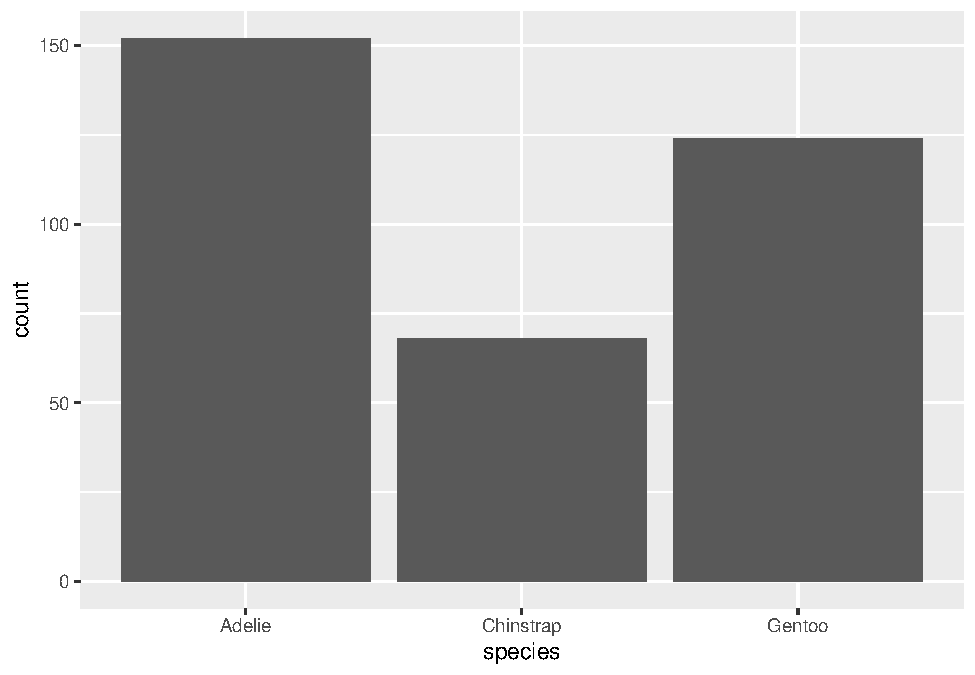
\includegraphics{intro_stats_files/figure-latex/unnamed-chunk-53-1.pdf}

We'll walk through this syntax step by step.

\begin{itemize}
\tightlist
\item
  The first argument of the \texttt{ggplot} command is the name of the tibble, in this case, \texttt{penguins}.
\item
  Next we define the aesthetics using \texttt{aes} and parentheses. Inside the parentheses, we assign any variables we want to plot to aesthetics of the graph. For this analysis, we are only interested in the variable \texttt{species} and for a bar chart, the categorical variable typically goes on the x-axis. That's why it says \texttt{x\ =\ species} inside the \texttt{aes} argument.
\item
  Finally, \texttt{ggplot} needs to know what kind of graph we want. Graph types are called ``geoms'' in the \texttt{ggplot} world, and \texttt{geom\_bar()} tells \texttt{ggplot} to add a ``bar chart layer''. Adding a layer is accomplished by literally typing a plus sign.
\end{itemize}

This can be modified somewhat to give proportions (relative frequencies) on the y-axis instead of counts. Unfortunately, the \texttt{ggplot} syntax is not very transparent here. My recommendation is to copy and paste the code below if you need to make a relative frequency bar chart in the future, making the necessary changes to the tibble and variable names, of course.

\begin{Shaded}
\begin{Highlighting}[]
\FunctionTok{ggplot}\NormalTok{(penguins, }\FunctionTok{aes}\NormalTok{(}\AttributeTok{x =}\NormalTok{ species, }\AttributeTok{y =}\NormalTok{ ..prop.., }\AttributeTok{group =} \DecValTok{1}\NormalTok{)) }\SpecialCharTok{+}
    \FunctionTok{geom\_bar}\NormalTok{()}
\end{Highlighting}
\end{Shaded}

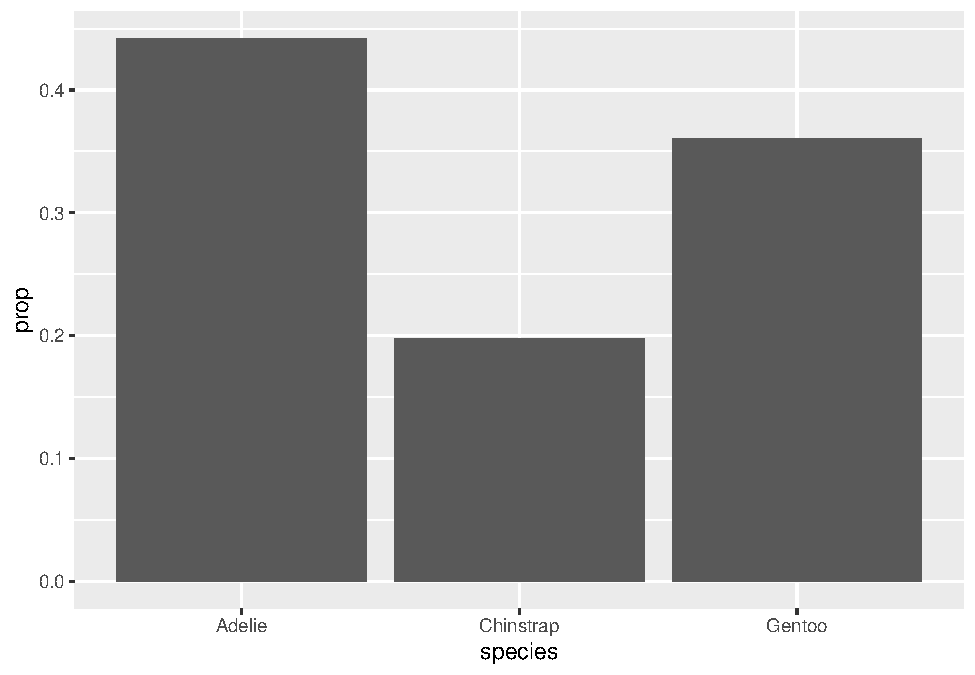
\includegraphics{intro_stats_files/figure-latex/unnamed-chunk-54-1.pdf}

These bar charts are the graphical analogues of a frequency table and a relative frequency table, respectively.

\hypertarget{exercise-4}{%
\paragraph*{Exercise 4}\label{exercise-4}}
\addcontentsline{toc}{paragraph}{Exercise 4}

In a sentence or two at most, describe the distribution of species in this data set.

Please write up your answer here.

\begin{center}\rule{0.5\linewidth}{0.5pt}\end{center}

What about pie charts? Just. Don't.

Seriously. Pie charts suck.\footnote{\url{https://medium.com/the-mission/to-pie-charts-3b1f57bcb34a}}

\hypertarget{categorical-summarizing-two}{%
\section{Summarizing two categorical variables}\label{categorical-summarizing-two}}

A table summarizing two categorical variables is called a \emph{contingency table} (or pivot table, or cross-tabulation, or probably several other terms as well).

For example, we might pose the following question: is the distribution of sex among penguins in our data more or less balanced across the three species?

When we work with two variables, typically we think of one variable as \emph{response} and the other as \emph{predictor}. The response variable is usually the variable of main interest. A predictor variable is another attribute that might predict or explain more about the response variable.

For example, our question is concerned with the sex distribution of penguins. We could create a relative frequency table of sex alone to see if male and female penguins are balanced in the data. In fact, you did that very thing above and saw that, indeed, there were roughly equal numbers of male and female penguins. But is that still true when we divide up the data into the three groups representing the separate species?

Two variables are called \emph{associated} when there is a relationship between them. For example, if sex and species were associated, then the distribution of sex would change depending on the species. Maybe one species of penguin had more females and another had fewer females. Our prediction of the sex distribution would change based on the value of the predictor variable \texttt{species}.

On the other hand, two variables that are not associated are called \emph{independent}. Independent variables are not related. If the sex distribution were the same across all species, then knowledge of the species would not change our predictions about the sex of a penguin. It wouldn't matter because there was no relationship between sex and species.

Most research questions that involve two or more variables are fundamentally questions of whether a response variable is associated with one or more predictor variables, or whether they are independent.

Let's check the contingency table. The \texttt{tabyl} command will place the first variable listed across the rows and the second one listed down the columns. It doesn't make any difference which variable is where, but to have a consistent rule on which we can rely, \textbf{let's always list the response variable first}.

\begin{Shaded}
\begin{Highlighting}[]
\FunctionTok{tabyl}\NormalTok{(penguins, sex, species)}
\end{Highlighting}
\end{Shaded}

\begin{verbatim}
##     sex Adelie Chinstrap Gentoo
##  female     73        34     58
##    male     73        34     61
##    <NA>      6         0      5
\end{verbatim}

Each column is a group, and our question is whether the distribution of sexes in each column is similar.

\hypertarget{exercise-5}{%
\paragraph*{Exercise 5}\label{exercise-5}}
\addcontentsline{toc}{paragraph}{Exercise 5}

Counts can be misleading. For example, there are 73 female Adelie penguins, but only 34 female Chinstrap penguins. Does that mean that Adelie penguins are more likely to be female than Chinstrap penguins? Why or why not?

Please write up your answer here.

\begin{center}\rule{0.5\linewidth}{0.5pt}\end{center}

A more fair way to compare across columns is to create relative frequencies. We can do this with a slightly different \texttt{adorn} command. The following code says that we want to compute column proportions (yes, I know the command is called \texttt{adorn\_percentages}, but these are proportions):

\begin{Shaded}
\begin{Highlighting}[]
\FunctionTok{tabyl}\NormalTok{(penguins, sex, species) }\SpecialCharTok{\%\textgreater{}\%}
    \FunctionTok{adorn\_percentages}\NormalTok{(}\StringTok{"col"}\NormalTok{)}
\end{Highlighting}
\end{Shaded}

\begin{verbatim}
##     sex     Adelie Chinstrap     Gentoo
##  female 0.48026316       0.5 0.46774194
##    male 0.48026316       0.5 0.49193548
##    <NA> 0.03947368       0.0 0.04032258
\end{verbatim}

If we actually want percentages, we need one more line of code. This command---\texttt{adorn\_pct\_formatting}---is the same as we used before with frequency tables.

\begin{Shaded}
\begin{Highlighting}[]
\FunctionTok{tabyl}\NormalTok{(penguins, sex, species) }\SpecialCharTok{\%\textgreater{}\%}
    \FunctionTok{adorn\_percentages}\NormalTok{(}\StringTok{"col"}\NormalTok{) }\SpecialCharTok{\%\textgreater{}\%}
    \FunctionTok{adorn\_pct\_formatting}\NormalTok{()}
\end{Highlighting}
\end{Shaded}

\begin{verbatim}
##     sex Adelie Chinstrap Gentoo
##  female  48.0%     50.0%  46.8%
##    male  48.0%     50.0%  49.2%
##    <NA>   3.9%      0.0%   4.0%
\end{verbatim}

Now we can see that each column adds up to 100\%. In other words, each species is now on equal footing, and only the distribution of sexes within each group matters.

\hypertarget{exercise-6a}{%
\paragraph*{Exercise 6(a)}\label{exercise-6a}}
\addcontentsline{toc}{paragraph}{Exercise 6(a)}

What percentage of Adelie penguins are male? What percentage of Chinstrap penguins are male? What percentage of Gentoo penguins are male?

Please write up your answer here.

\hypertarget{exercise-6b}{%
\paragraph*{Exercise 6(b)}\label{exercise-6b}}
\addcontentsline{toc}{paragraph}{Exercise 6(b)}

Does sex appear to be associated with species for the penguins in this data set? Or are these variables independent?

Please write up your answer here.

\begin{center}\rule{0.5\linewidth}{0.5pt}\end{center}

The islands of Antarctica on which the penguins were observed and measured are recorded in the variable called \texttt{island}. Is the distribution of the three species of penguin the same (or similar) on the three islands?

\hypertarget{exercise-7a}{%
\paragraph*{Exercise 7(a)}\label{exercise-7a}}
\addcontentsline{toc}{paragraph}{Exercise 7(a)}

Choosing which variables play the roles of response and predictor can be tricky. For the question above, with \texttt{species} and \texttt{island}, which is response and which is predictor?

One way to think about this is to ask the following two questions and see which one is closer to the question asked:

\begin{itemize}
\tightlist
\item
  Given information about the species, are you interested in which island the penguin lives on? If so, \texttt{species} is a predictor and \texttt{island} is response. (You are using \texttt{species} to predict \texttt{island}.)
\item
  Given information about the island, are you interested in the species of the penguin? If so, \texttt{island} is a predictor and \texttt{species} is response. (You are using \texttt{island} to predict \texttt{species}.)
\end{itemize}

Please write up your answer here.

\hypertarget{exercise-7b}{%
\paragraph*{Exercise 7(b)}\label{exercise-7b}}
\addcontentsline{toc}{paragraph}{Exercise 7(b)}

Create a contingency table with percentages. List \texttt{species} first, followed by \texttt{island}. (Hey, that's hint in case you need to go back and change your answer to part (a).)

\begin{Shaded}
\begin{Highlighting}[]
\CommentTok{\# Add code here to create a contingency table with percentages.}
\end{Highlighting}
\end{Shaded}

\hypertarget{exercise-7c}{%
\paragraph*{Exercise 7(c)}\label{exercise-7c}}
\addcontentsline{toc}{paragraph}{Exercise 7(c)}

Finally, comment on the association or independence of the two variables.

Please write up your answer here.

\hypertarget{categorical-graphing-two}{%
\section{Graphing two categorical variables}\label{categorical-graphing-two}}

A somewhat effective way to display two categorical variables is with a side-by-side bar chart. Here is the \texttt{ggplot} code for the relationship between \texttt{sex} and \texttt{species}.

\begin{Shaded}
\begin{Highlighting}[]
\FunctionTok{ggplot}\NormalTok{(penguins, }\FunctionTok{aes}\NormalTok{(}\AttributeTok{fill =}\NormalTok{ sex, }\AttributeTok{x =}\NormalTok{ species)) }\SpecialCharTok{+}
    \FunctionTok{geom\_bar}\NormalTok{(}\AttributeTok{position =} \StringTok{"dodge"}\NormalTok{)}
\end{Highlighting}
\end{Shaded}

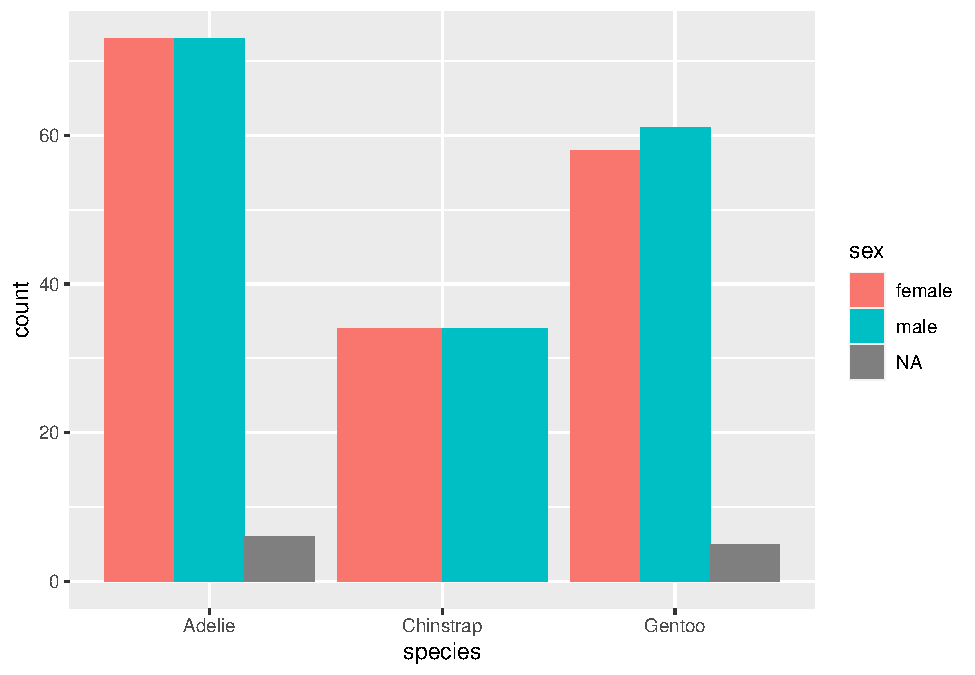
\includegraphics{intro_stats_files/figure-latex/unnamed-chunk-59-1.pdf}

This is somewhat different from the first \texttt{ggplot} example you saw above, so let's take a moment to go through it.

\begin{itemize}
\tightlist
\item
  The first argument is the data frame \texttt{penguins}; no mystery there.
\item
  The second aesthetic \texttt{x\ =\ species} also makes a lot of sense. As \texttt{species} is our predictor variable---we're using species to group the penguins, and then within each species, we're interested in the sex distribution---\texttt{species} goes on the x-axis.
\item
  However, \texttt{sex} does not go on the y-axis! (This is a very common mistake for novices.) The y-axis of a bar chart is always a count or a proportion/percentage, so no variable should ever go on the y-axis of a bar chart. In that case, how does \texttt{sex} enter the picture? Through the use of color! The aesthetic \texttt{fill\ =\ sex} says to use the \texttt{sex} variable to shade or ``fill'' the bars with different colors. You'll also notice that \texttt{ggplot} makes a legend automatically with the colors so you can see which color corresponds to which value (in this case, ``female'', ``male'', or ``NA'' for the missing data).
\end{itemize}

Another unusual feature is the argument \texttt{position\ =\ "dodge"} in the \texttt{geom\_bar} layer. Let's see what happens if we remove it.

\begin{Shaded}
\begin{Highlighting}[]
\FunctionTok{ggplot}\NormalTok{(penguins, }\FunctionTok{aes}\NormalTok{(}\AttributeTok{fill =}\NormalTok{ sex, }\AttributeTok{x =}\NormalTok{ species)) }\SpecialCharTok{+} 
    \FunctionTok{geom\_bar}\NormalTok{()}
\end{Highlighting}
\end{Shaded}

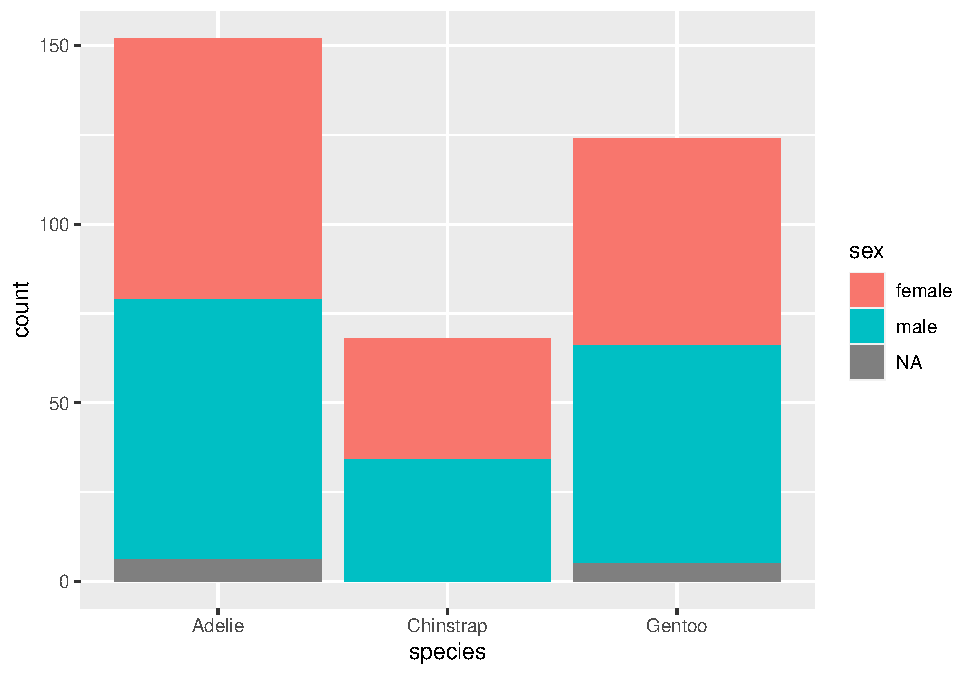
\includegraphics{intro_stats_files/figure-latex/unnamed-chunk-60-1.pdf}

We get a stacked bar chart! This is another popular way of displaying two categorical variables, but we don't tend to prefer it. Notice how difficult it is to compare the number of females across species; since there is no common baseline for the red segments of each bar, it is harder to determine which ones are bigger or smaller. (In this case, it's fairly clear, but there are plenty of data sets for which the counts might be a lot closer.)

So let's agree to use side-by-side bar charts. There is still one aspect of the side-by-side bar chart that is misleading, though. For example, the red bar for Adelie penguins is bigger than the red bar for Gentoo penguins. Does this mean Adelie penguins are more likely to be female?

This is the same issue we identified in an exercise above. To fix this problem, a better option here would be to use relative frequencies (i.e., proportions/percentages within each group) instead of counts on the y-axis. This is analogous to using proportions/percentages in a contingency table. Unfortunately, it is rather difficult to do this with \texttt{ggplot}. A compromise is available: by using \texttt{position\ =\ fill}, you can create a stacked bar chart that scales every group to 100\%. Making comparisons across groups can still be hard, as explained above for any kind of stacked bar chart, but it works okay if there are only two categories in the response variable (as is almost the case with \texttt{sex} here, although the missing data distorts things a little at the bottom).

\begin{Shaded}
\begin{Highlighting}[]
\FunctionTok{ggplot}\NormalTok{(penguins, }\FunctionTok{aes}\NormalTok{(}\AttributeTok{fill =}\NormalTok{ sex, }\AttributeTok{x =}\NormalTok{ species)) }\SpecialCharTok{+}
    \FunctionTok{geom\_bar}\NormalTok{(}\AttributeTok{position =} \StringTok{"fill"}\NormalTok{)}
\end{Highlighting}
\end{Shaded}

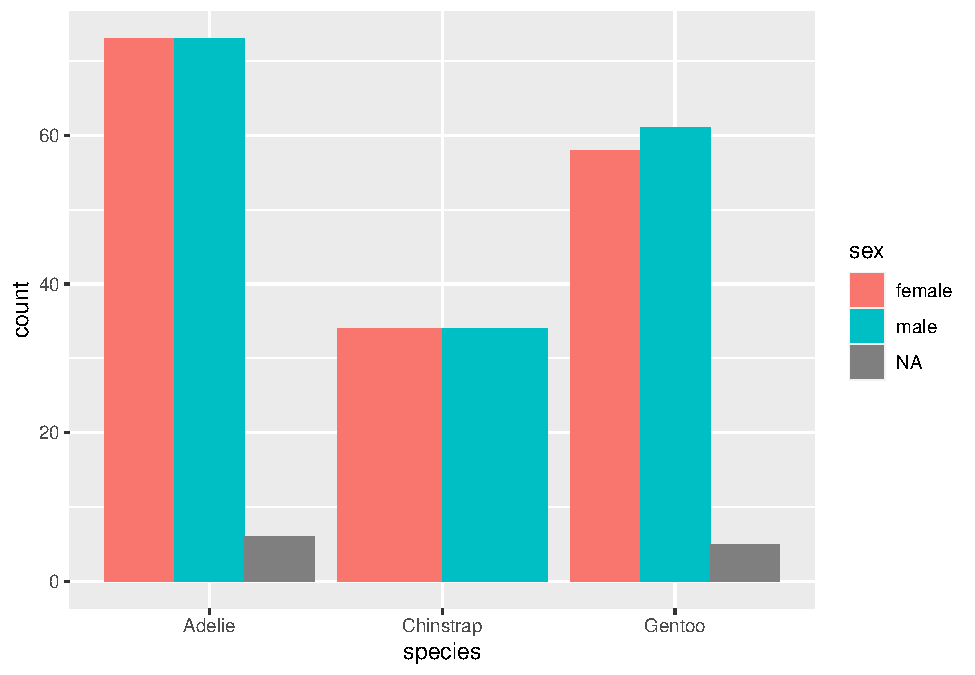
\includegraphics{intro_stats_files/figure-latex/unnamed-chunk-61-1.pdf}

This graph does correctly show that the sexes are pretty much equally balances across all three species.

\hypertarget{exercise-8a}{%
\paragraph*{Exercise 8(a)}\label{exercise-8a}}
\addcontentsline{toc}{paragraph}{Exercise 8(a)}

Using \texttt{species} and \texttt{island}, create a side-by-side bar chart. Be careful, though, to change the sample code above to make sure \texttt{species} is now the response variable (using the \texttt{fill} aesthetic) and that \texttt{island} is the explanatory variable (using \texttt{x}). (Hey, that's another hint to go back and look at the previous exercise and make sure you got part (a) right!)

\begin{Shaded}
\begin{Highlighting}[]
\CommentTok{\# Add code here to make a side{-}by{-}side bar chart.}
\end{Highlighting}
\end{Shaded}

\hypertarget{exercise-8b}{%
\paragraph*{Exercise 8(b)}\label{exercise-8b}}
\addcontentsline{toc}{paragraph}{Exercise 8(b)}

Comment on the association or independence of the two variables.

Please write up your answer here.

\hypertarget{categorical-recoding}{%
\section{Recoding factor variables}\label{categorical-recoding}}

As mentioned earlier, there are situations where a categorical variable is not recorded in R as a factor variable. Let's look at the \texttt{year} variable:

\begin{Shaded}
\begin{Highlighting}[]
\FunctionTok{glimpse}\NormalTok{(penguins}\SpecialCharTok{$}\NormalTok{year)}
\end{Highlighting}
\end{Shaded}

\begin{verbatim}
##  int [1:344] 2007 2007 2007 2007 2007 2007 2007 2007 2007 2007 ...
\end{verbatim}

These appear as integers. Yes, years are whole numbers, but why might this variable be treated as categorical data and not numerical data?

\hypertarget{exercise-9a}{%
\paragraph*{Exercise 9(a)}\label{exercise-9a}}
\addcontentsline{toc}{paragraph}{Exercise 9(a)}

Use the \texttt{tabyl} command to create a frequency table for \texttt{year}.

\begin{Shaded}
\begin{Highlighting}[]
\CommentTok{\# Add code here to make a frequency table for year.}
\end{Highlighting}
\end{Shaded}

\hypertarget{exercise-9b}{%
\paragraph*{Exercise 9(b)}\label{exercise-9b}}
\addcontentsline{toc}{paragraph}{Exercise 9(b)}

Why is \texttt{year} better thought of as categorical data and not numerical data (at least for this data set---we're not claiming years should always be treated as categorical)?

Please write up your answer here.

\begin{center}\rule{0.5\linewidth}{0.5pt}\end{center}

While the \texttt{tabyl} command seemed to work just fine with the \texttt{year} data in integer format, there are other commands that will not work so well. For example, \texttt{ggplot} often fails to do the right thing when a categorical variable is coded as a number. Therefore, we need a way to change numerically coded variables to factors.

The code below uses a command called \texttt{mutate} that takes an old variable and creates a new variable. (You'll learn more about this command in a later chapter. For now, you can just copy and paste this code if you need it again.) The name of the new variable can be anything we want; we'll just call it \texttt{year\_fct}. Then the real work is being done by the \texttt{as\_factor} command that concerts the numeric \texttt{year} variable into a factor variable.

Observe the effect below:

\begin{Shaded}
\begin{Highlighting}[]
\NormalTok{penguins }\OtherTok{\textless{}{-}}\NormalTok{ penguins }\SpecialCharTok{\%\textgreater{}\%}
    \FunctionTok{mutate}\NormalTok{(}\AttributeTok{year\_fct =} \FunctionTok{as\_factor}\NormalTok{(year))}
\FunctionTok{glimpse}\NormalTok{(penguins)}
\end{Highlighting}
\end{Shaded}

\begin{verbatim}
## Rows: 344
## Columns: 9
## $ species           <fct> Adelie, Adelie, Adelie, Adelie, Adelie, Adelie, Adel~
## $ island            <fct> Torgersen, Torgersen, Torgersen, Torgersen, Torgerse~
## $ bill_length_mm    <dbl> 39.1, 39.5, 40.3, NA, 36.7, 39.3, 38.9, 39.2, 34.1, ~
## $ bill_depth_mm     <dbl> 18.7, 17.4, 18.0, NA, 19.3, 20.6, 17.8, 19.6, 18.1, ~
## $ flipper_length_mm <int> 181, 186, 195, NA, 193, 190, 181, 195, 193, 190, 186~
## $ body_mass_g       <int> 3750, 3800, 3250, NA, 3450, 3650, 3625, 4675, 3475, ~
## $ sex               <fct> male, female, female, NA, female, male, female, male~
## $ year              <int> 2007, 2007, 2007, 2007, 2007, 2007, 2007, 2007, 2007~
## $ year_fct          <fct> 2007, 2007, 2007, 2007, 2007, 2007, 2007, 2007, 2007~
\end{verbatim}

\hypertarget{exercise-10a}{%
\paragraph*{Exercise 10(a)}\label{exercise-10a}}
\addcontentsline{toc}{paragraph}{Exercise 10(a)}

Make a contingency table of the species measured in each year using counts. Use the \texttt{species} variable first, followed by the new factor variable \texttt{year\_fct}. (Think about why that order makes sense. \textbf{We will always list the response variable first so that the categories of interest will be the rows and the groups will be the columns.})

\begin{Shaded}
\begin{Highlighting}[]
\CommentTok{\# Add code here to make a contingency table for species and year with counts.}
\end{Highlighting}
\end{Shaded}

\hypertarget{exercise-10b}{%
\paragraph*{Exercise 10(b)}\label{exercise-10b}}
\addcontentsline{toc}{paragraph}{Exercise 10(b)}

Make a contingency table of the species measured in each year using column percentages (\emph{not} proportions). (Again, be sure to use the new factor variable \texttt{year\_fct}, not the old variable \texttt{year}.)

\begin{Shaded}
\begin{Highlighting}[]
\CommentTok{\# Add code here to make a contingency table for species and year with percentages.}
\end{Highlighting}
\end{Shaded}

\hypertarget{exercise-10c}{%
\paragraph*{Exercise 10(c)}\label{exercise-10c}}
\addcontentsline{toc}{paragraph}{Exercise 10(c)}

How similar or dissimilar are the distributions of species across the three years of the study?

Please write up your answer here.

\hypertarget{categorical-pub}{%
\section{Publication-ready graphics}\label{categorical-pub}}

Let's go back to the first relative frequency bar chart from this chapter.

\begin{Shaded}
\begin{Highlighting}[]
\FunctionTok{ggplot}\NormalTok{(penguins, }\FunctionTok{aes}\NormalTok{(}\AttributeTok{x =}\NormalTok{ species, }\AttributeTok{y =}\NormalTok{ ..prop.., }\AttributeTok{group =} \DecValTok{1}\NormalTok{)) }\SpecialCharTok{+}
    \FunctionTok{geom\_bar}\NormalTok{()}
\end{Highlighting}
\end{Shaded}

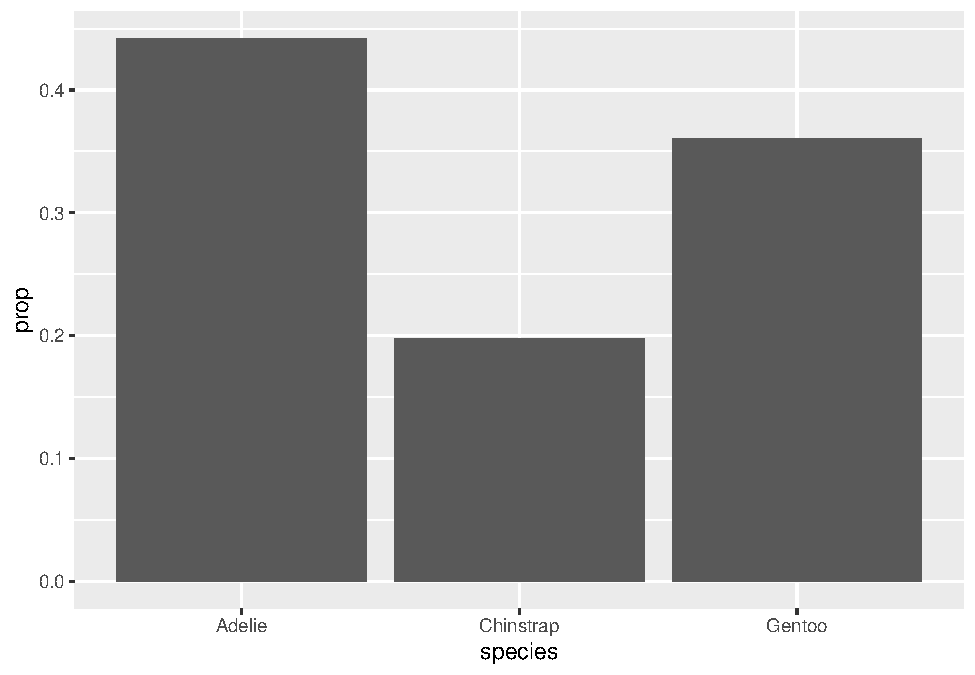
\includegraphics{intro_stats_files/figure-latex/unnamed-chunk-68-1.pdf}

The variable name \texttt{species} is already informative, but the y-axis is labeled with ``prop''. Also note that this graph could use a title. We can do all this with \texttt{labs} (for labels). Observe:

\begin{Shaded}
\begin{Highlighting}[]
\FunctionTok{ggplot}\NormalTok{(penguins, }\FunctionTok{aes}\NormalTok{(}\AttributeTok{x =}\NormalTok{ species, }\AttributeTok{y =}\NormalTok{ ..prop.., }\AttributeTok{group =} \DecValTok{1}\NormalTok{)) }\SpecialCharTok{+}
    \FunctionTok{geom\_bar}\NormalTok{() }\SpecialCharTok{+}
    \FunctionTok{labs}\NormalTok{(}\AttributeTok{title =} \StringTok{"Distribution of species"}\NormalTok{,}
         \AttributeTok{y =} \StringTok{"Proportion"}\NormalTok{,}
         \AttributeTok{x =} \StringTok{"Species"}\NormalTok{)}
\end{Highlighting}
\end{Shaded}

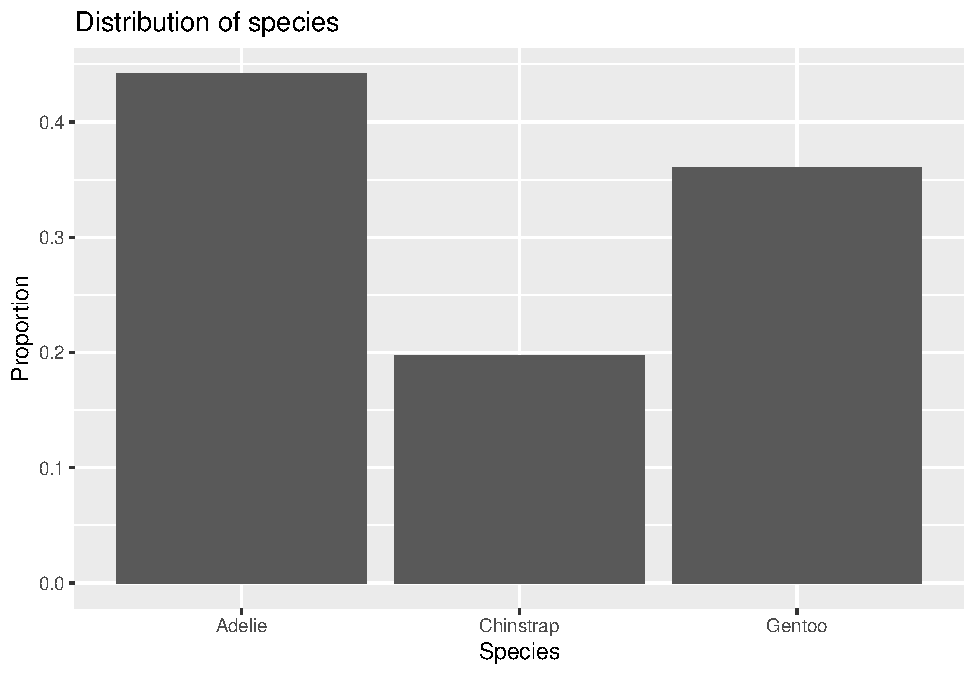
\includegraphics{intro_stats_files/figure-latex/unnamed-chunk-69-1.pdf}

\hypertarget{exercise-11}{%
\paragraph*{Exercise 11}\label{exercise-11}}
\addcontentsline{toc}{paragraph}{Exercise 11}

Modify the following side-by-side bar chart by adding a title and labels for both the fill variable and the x-axis variable. (Hint: you can use \texttt{fill\ =\ sex} inside the \texttt{labs} command just like you used \texttt{title}, \texttt{y}, and \texttt{x}.)

\begin{Shaded}
\begin{Highlighting}[]
\CommentTok{\# Modify the following side{-}by{-}side bar chart by adding a title and }
\CommentTok{\# labels for both the x{-}axis and the fill variable.}
\FunctionTok{ggplot}\NormalTok{(penguins, }\FunctionTok{aes}\NormalTok{(}\AttributeTok{fill =}\NormalTok{ sex, }\AttributeTok{x =}\NormalTok{ species)) }\SpecialCharTok{+}
    \FunctionTok{geom\_bar}\NormalTok{(}\AttributeTok{position =} \StringTok{"dodge"}\NormalTok{)}
\end{Highlighting}
\end{Shaded}

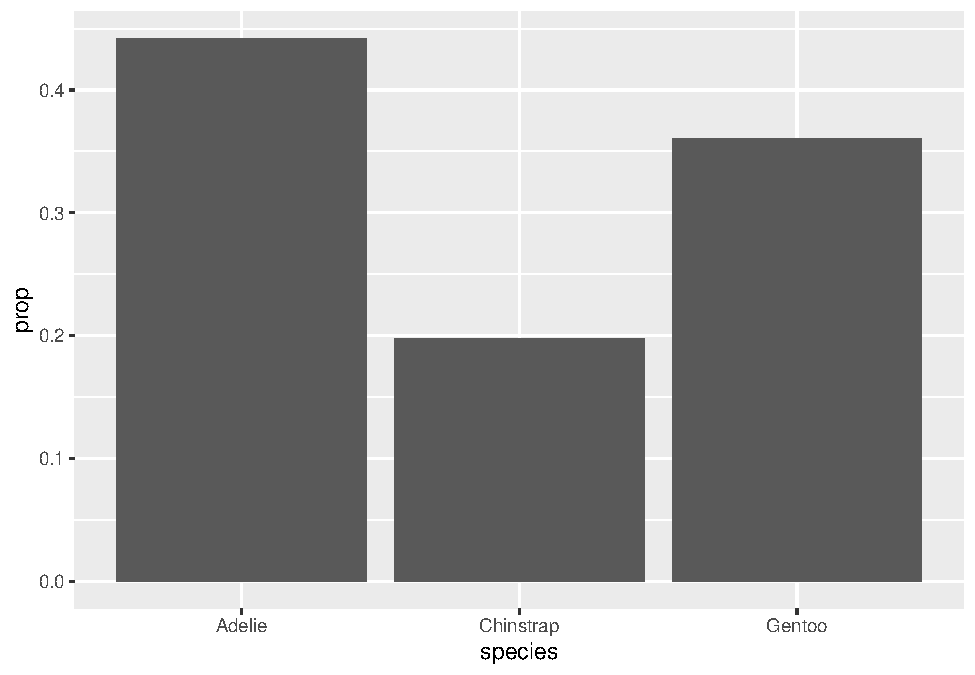
\includegraphics{intro_stats_files/figure-latex/unnamed-chunk-70-1.pdf}

\hypertarget{categorical-summary}{%
\section{Plotting summary data}\label{categorical-summary}}

Everything we did above was summarizing \emph{raw data}; that is, the data consisted of all the observations for each individual penguin. Often, though, when you find data out in the wild, that data will be summarized into a table already and you may not have access to the raw data.

For example, let's suppose that you found some data online, but it looked like this:

\begin{longtable}[]{@{}ll@{}}
\toprule()
species & count \\
\midrule()
\endhead
Adelie & 152 \\
Chinstrap & 68 \\
Gentoo & 124 \\
\bottomrule()
\end{longtable}

This raises two questions:

\begin{enumerate}
\def\labelenumi{\arabic{enumi}.}
\tightlist
\item
  How would you get this data into R?
\item
  How would you plot the data?
\end{enumerate}

To answer the first question, we show you how to create your own tibble. Here is the syntax:

\begin{Shaded}
\begin{Highlighting}[]
\NormalTok{penguin\_species\_table }\OtherTok{\textless{}{-}} \FunctionTok{tibble}\NormalTok{(}
    \AttributeTok{species =} \FunctionTok{c}\NormalTok{(}\StringTok{"Adelie"}\NormalTok{, }\StringTok{"Chinstrap"}\NormalTok{, }\StringTok{"Gentoo"}\NormalTok{),}
    \AttributeTok{count =} \FunctionTok{c}\NormalTok{(}\DecValTok{152}\NormalTok{, }\DecValTok{68}\NormalTok{, }\DecValTok{124}\NormalTok{)}
\NormalTok{)}
\NormalTok{penguin\_species\_table}
\end{Highlighting}
\end{Shaded}

\begin{verbatim}
## # A tibble: 3 x 2
##   species   count
##   <chr>     <dbl>
## 1 Adelie      152
## 2 Chinstrap    68
## 3 Gentoo      124
\end{verbatim}

Basically, the \texttt{tibble} command creates a new tibble. Then each column of data must be entered manually as a ``vector'' using the \texttt{c} to group all the data values together for each column. Be careful about the placement of quotation marks, commas, and parentheses.

Once we have our summary data, we want to make a bar chart. But this won't work:

\begin{Shaded}
\begin{Highlighting}[]
\FunctionTok{ggplot}\NormalTok{(penguin\_species\_table, }\FunctionTok{aes}\NormalTok{(}\AttributeTok{x =}\NormalTok{ species)) }\SpecialCharTok{+}
    \FunctionTok{geom\_bar}\NormalTok{()}
\end{Highlighting}
\end{Shaded}

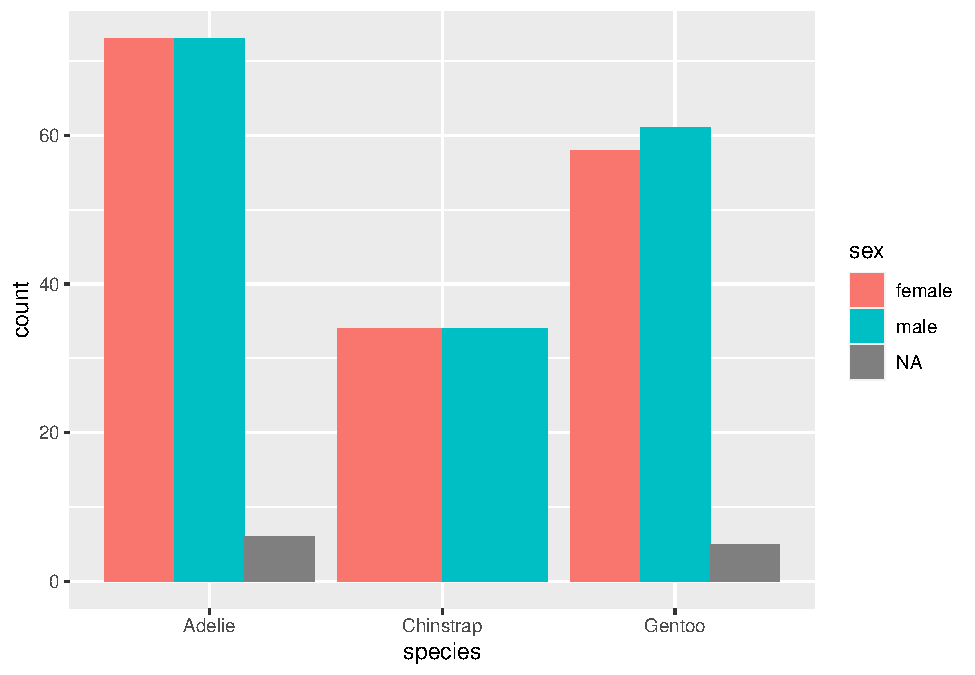
\includegraphics{intro_stats_files/figure-latex/unnamed-chunk-72-1.pdf}

\hypertarget{exercise-12}{%
\paragraph*{Exercise 12}\label{exercise-12}}
\addcontentsline{toc}{paragraph}{Exercise 12}

Explain what went wrong with the previous command? Why does \texttt{ggplot} think that each species has count 1?

Please write up your answer here.

\begin{center}\rule{0.5\linewidth}{0.5pt}\end{center}

Instead, we need to use \texttt{geom\_col}. This works a lot like \texttt{geom\_bar} except that it also requires a \texttt{y} value in its aesthetics to force the command to look for the counts in some other variable in the data.

\begin{Shaded}
\begin{Highlighting}[]
\FunctionTok{ggplot}\NormalTok{(penguin\_species\_table, }\FunctionTok{aes}\NormalTok{(}\AttributeTok{x =}\NormalTok{ species, }\AttributeTok{y =}\NormalTok{ count)) }\SpecialCharTok{+}
    \FunctionTok{geom\_col}\NormalTok{()}
\end{Highlighting}
\end{Shaded}

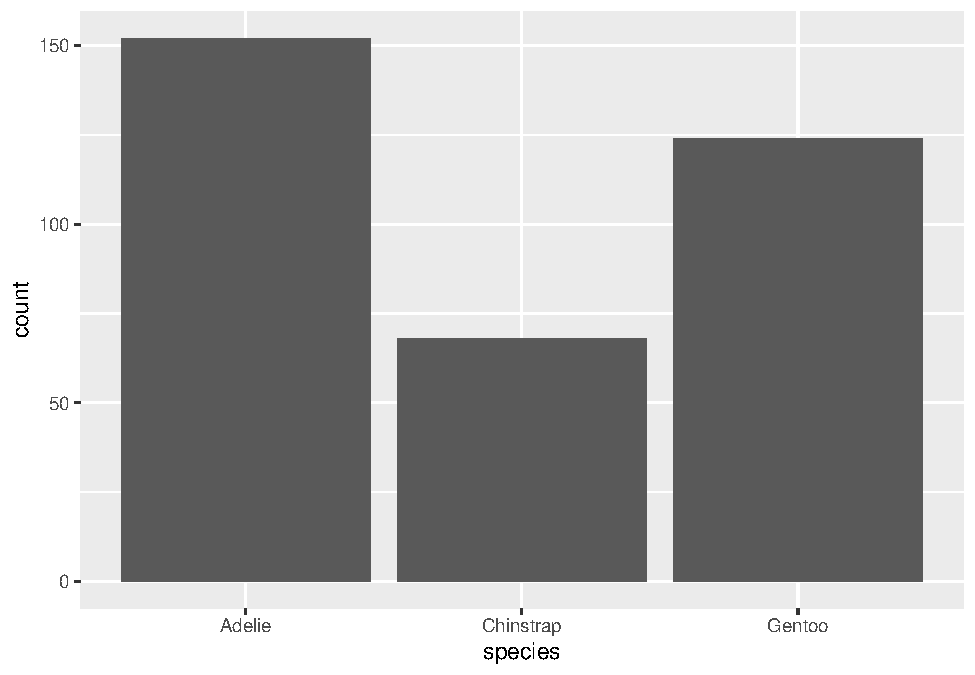
\includegraphics{intro_stats_files/figure-latex/unnamed-chunk-73-1.pdf}

\hypertarget{exercise-13a}{%
\paragraph*{Exercise 13(a)}\label{exercise-13a}}
\addcontentsline{toc}{paragraph}{Exercise 13(a)}

Use the \texttt{tabyl} command to create a frequency table for \texttt{island}.

\begin{Shaded}
\begin{Highlighting}[]
\CommentTok{\# Add code here to create a frequency table for island}
\end{Highlighting}
\end{Shaded}

\hypertarget{exercise-13b}{%
\paragraph*{Exercise 13(b)}\label{exercise-13b}}
\addcontentsline{toc}{paragraph}{Exercise 13(b)}

Use the \texttt{tibble} command to create a new tibble manually that contains the frequency data for the \texttt{island} variable. It should have two columns, one called \texttt{island} and the other called \texttt{count}. Name it \texttt{penguin\_island\_table}.

\begin{Shaded}
\begin{Highlighting}[]
\CommentTok{\# Add code here to create a tibble with frequency data for island}
\end{Highlighting}
\end{Shaded}

\hypertarget{exercise-13c}{%
\paragraph*{Exercise 13(c)}\label{exercise-13c}}
\addcontentsline{toc}{paragraph}{Exercise 13(c)}

Use \texttt{ggplot} with \texttt{geom\_col} to create a bar chart for island.

\begin{Shaded}
\begin{Highlighting}[]
\CommentTok{\# Add code here to create a bar chart for island}
\end{Highlighting}
\end{Shaded}

\hypertarget{categorical-conclusion}{%
\section{Conclusion}\label{categorical-conclusion}}

You can summarize a single categorical variable using a frequency table. For only one categorical variable, a graph is usually overkill, but if you really want a graph, the bar chart is the best option. Both raw counts and proportions/percentages can be useful.

We use contingency tables to summarize two categorical variables. Unless groups are of equal size, raw counts can be incredibly misleading here. You should include proportions/percentages to be able to compare the distributions across groups. If the proportions/percentages are roughly the same, the variables are more likely to be independent, whereas if the proportions/percentages are different, there may be an association between the variables. For graphing, the best choice is usually a side-by-side bar chart. A stacked bar chart will also work, especially if using relative frequencies on the y-axis, but it can be hard to compare across groups when the response variable has three or more categories.

Sometimes we come across categorical data that is recorded using numbers. Many R commands will not work properly if they expect factors and receive numbers, so we use the \texttt{mutate} command to create a new variable along with \texttt{as\_factor} to convert the numbers to categories.

Sometimes we come across summary data instead of raw data. We can then manually create tibbles with that summary data and use \texttt{geom\_col} instead of \texttt{geom\_bar} to graph it.

\hypertarget{categorical-prep}{%
\subsection{Preparing and submitting your assignment}\label{categorical-prep}}

\begin{enumerate}
\def\labelenumi{\arabic{enumi}.}
\tightlist
\item
  From the ``Run'' menu, select ``Restart R and Run All Chunks''.
\item
  Deal with any code errors that crop up. Repeat steps 1---2 until there are no more code errors.
\item
  Spell check your document by clicking the icon with ``ABC'' and a check mark.
\item
  Hit the ``Preview'' button one last time to generate the final draft of the \texttt{.nb.html} file.
\item
  Proofread the HTML file carefully. If there are errors, go back and fix them, then repeat steps 1--5 again.
\end{enumerate}

If you have completed this chapter as part of a statistics course, follow the directions you receive from your professor to submit your assignment.

\hypertarget{numerical}{%
\chapter{Numerical data}\label{numerical}}

2.0

\hypertarget{functions-introduced-in-this-chapter-3}{%
\subsection*{Functions introduced in this chapter}\label{functions-introduced-in-this-chapter-3}}
\addcontentsline{toc}{subsection}{Functions introduced in this chapter}

\texttt{mean}, \texttt{sd}, \texttt{var}, \texttt{median}, \texttt{sort}, \texttt{IQR}, \texttt{quantile}, \texttt{summary}, \texttt{min}, \texttt{max}, \texttt{geom\_histogram}, \texttt{geom\_point}, \texttt{geom\_boxplot}, \texttt{facet\_grid}

\hypertarget{numerical-intro}{%
\section{Introduction}\label{numerical-intro}}

In this chapter, we'll learn about numerical data and how to summarize it through summary statistics and graphs.

\hypertarget{numerical-install}{%
\subsection{Install new packages}\label{numerical-install}}

There are no new packages used in this chapter.

\hypertarget{numerical-download}{%
\subsection{Download the R notebook file}\label{numerical-download}}

Check the upper-right corner in RStudio to make sure you're in your \texttt{intro\_stats} project. Then click on the following link to download this chapter as an R notebook file (\texttt{.Rmd}).

https://vectorposse.github.io/intro\_stats/chapter\_downloads/04-numerical\_data.Rmd

Once the file is downloaded, move it to your project folder in RStudio and open it there.

\hypertarget{numerical-restart}{%
\subsection{Restart R and run all chunks}\label{numerical-restart}}

In RStudio, select ``Restart R and Run All Chunks'' from the ``Run'' menu.

\hypertarget{numerical-load}{%
\subsection{Load packages}\label{numerical-load}}

We load the \texttt{tidyverse} package to get \texttt{ggplot2} and the \texttt{palmerpenguins} package to work with the penguin data.

\begin{Shaded}
\begin{Highlighting}[]
\FunctionTok{library}\NormalTok{(tidyverse)}
\FunctionTok{library}\NormalTok{(palmerpenguins)}
\end{Highlighting}
\end{Shaded}

\hypertarget{numerical-notation}{%
\section{A note about mathematical notation}\label{numerical-notation}}

From time to time, we will use mathematical notation that can't be typed directly on the keyboard. For example, let's suppose we want to typeset the quadratic formula, which involves a complicated fraction as well as a square root symbol.

When such notation appears, it will be surrounded by double dollar signs as follows:

\[
x = \frac{-b \pm \sqrt{b^{2} - 4ac}}{2a}
\]

The R Notebook will interpret this special mathematical notation and render it on the screen as well as in the HTML document.\footnote{This notation is part of a mathematical document preparation system called LaTeX, pronounced ``Lay-tek'' (not like the rubbery substance).} If the nicely formatted formula does not appear on your screen, place your cursor anywhere inside the math formula and hit Ctrl-Enter or Cmd-Enter (PC or Mac respectively).

Sometimes, we want such math to appear inline. We can do this with single dollar signs. For example, the distance formula is \(d = \sqrt{(x_{2} - x_{1})^{2} + (y_{2} - y_{1})^{2}}\), a fact you may have learned a long time ago.

This will \emph{not} render visually in the R Notebook, but it will show up in the HTML file. If you want to check that it worked properly without having to preview the HTML, you can either hover your cursor over the math formula and wait a second, or you can place your cursor anywhere inside the math formula and hit Ctrl-Enter or Cmd-Enter (PC or Mac respectively) to see a pop-up window previewing the mathematical content properly formatted.

You will be shown examples of any mathematical notation you need to use in any given chapter, so feel free to copy/paste/modify any math notation you need.

\hypertarget{numerical-statistics}{%
\section{Statistics}\label{numerical-statistics}}

The word ``statistics'' has several meanings. On one hand, it's an entire field of study, as in the subject of this course. More specifically, though, a ``statistic'' is any kind of numerical summary of data. While there are many ways to summarize data, they mostly fall into two main flavors: measures of \emph{center} and measures of \emph{spread}. Measures of center try to estimate some kind of average, middle, or common value in data. Measures of spread try to estimate something like the width, range, variability, or uncertainty of data.

There are two pairs of measurements that we will learn about in this chapter: the mean/standard deviation, and the median/IQR.

\hypertarget{numerical-mean-sd}{%
\subsection{Mean and standard deviation}\label{numerical-mean-sd}}

The first pair of the summary statistics we'll discuss consists of the mean and the standard deviation.

The \emph{mean} of a variable \(y\)---denoted \(\bar{y}\) and pronounced ``y bar''---is calculated by summing all the values of the variable, and dividing by the total number of observations. In formula form, this is

\[
\bar{y} = \frac{\sum y}{n}.
\]

This is a measure of center since it estimates the ``middle'' of a set of numbers. It is calculated in R using the \texttt{mean} command.

Throughout this chapter, we will be using the \texttt{penguins} data set. (If you need a reminder, look at the help file for \texttt{penguins} using one of the methods discussed in Chapter 2.)

If we want to calculate the mean body mass of our penguins (in grams), we type the following:

\begin{Shaded}
\begin{Highlighting}[]
\FunctionTok{mean}\NormalTok{(penguins}\SpecialCharTok{$}\NormalTok{body\_mass\_g)}
\end{Highlighting}
\end{Shaded}

\begin{verbatim}
## [1] NA
\end{verbatim}

Unfortunately, this didn't give us an answer. As you may recall from previous chapters, this is because we are missing several values of body mass in this data. We need an extra piece of code to tell R to ignore that missing data and give us the mean of the valid data.

\begin{Shaded}
\begin{Highlighting}[]
\FunctionTok{mean}\NormalTok{(penguins}\SpecialCharTok{$}\NormalTok{body\_mass\_g, }\AttributeTok{na.rm =} \ConstantTok{TRUE}\NormalTok{)}
\end{Highlighting}
\end{Shaded}

\begin{verbatim}
## [1] 4201.754
\end{verbatim}

(The term \texttt{na.rm} stands for ``NA remove''.)

We never leave such numbers without interpretation. In a full, contextually meaningful sentence, we might say, ``The mean body mass of this group of penguins is approximately 4200 grams.''

Notice that we mentioned the penguins, placing this number in context, and we mentioned the units of measurement, grams. (Otherwise, what would this number mean? 4200 pounds? Okay, probably not, but you should always mention the units of measurement.) Also notice that we rounded the final value. A gram is a very small unit of measurement, so there is no need to report this value to many decimal places.

If we use inline code, we can say, ``The mean body mass of this group of penguins is 4201.754386 grams.'' There are ways of rounding this number as well, but it's a bit of a hassle to do so in inline code.

The corresponding measure of spread is the \emph{standard deviation}. Usually this is called \(s\) and is calculated using a much more complicated formula:

\[
s = \sqrt{\frac{\sum (y - \bar{y})^2}{n - 1}}.
\]

This is a measure of spread because the \((y - \bar{y})\) term measures the how far away each data point is from the mean.

In R, this is calculated with the \texttt{sd} command. Again, we'll need to add \texttt{na.rm\ =\ TRUE}.

\begin{Shaded}
\begin{Highlighting}[]
\FunctionTok{sd}\NormalTok{(penguins}\SpecialCharTok{$}\NormalTok{body\_mass\_g, }\AttributeTok{na.rm =} \ConstantTok{TRUE}\NormalTok{)}
\end{Highlighting}
\end{Shaded}

\begin{verbatim}
## [1] 801.9545
\end{verbatim}

``The standard deviation of this group of penguins is about 801 grams.''

Or using inline code:

``The standard deviation of this group of penguins is 801.9545357 grams.''

The mean and the standard deviation should always be reported together. One without the other is incomplete and potentially misleading.

Another related measurement is the \emph{variance}, but this is nothing more than the standard deviation squared:

\[
s^2 = \frac{\sum (y - \bar{y})^2}{n - 1}.
\]

(Compare this formula to the one for the standard deviation. Nothing has changed except for the removal of the square root.) We rarely use the variance in an introductory stats class because it's not as interpretable as the standard deviation. The main reason for this is units. If the data units are grams, then both the mean and the standard deviation are also reported in grams. The variance has units of ``grams squared'', but what does that even mean? If you need to calculate the variance in R, the command is \texttt{var}.

\begin{Shaded}
\begin{Highlighting}[]
\FunctionTok{var}\NormalTok{(penguins}\SpecialCharTok{$}\NormalTok{body\_mass\_g, }\AttributeTok{na.rm =} \ConstantTok{TRUE}\NormalTok{)}
\end{Highlighting}
\end{Shaded}

\begin{verbatim}
## [1] 643131.1
\end{verbatim}

You can check and see that the number above really is just 801.9545357 squared. Regarding the inline code in the previous sentence, remember, in the R Notebook, you can click inside the inline code and hit Ctrl-Enter or Cmd-Enter. In the HTML document, the number will be calculated and will magically appear.

\hypertarget{numerical-median-iqr}{%
\subsection{Median and IQR}\label{numerical-median-iqr}}

Another choice for measuring the center and spread of a data set is the median and the IQR.

The median is just the middle value if the list of values is ordered. In R, it is calculated using the \texttt{median} command.

\begin{Shaded}
\begin{Highlighting}[]
\FunctionTok{median}\NormalTok{(penguins}\SpecialCharTok{$}\NormalTok{body\_mass\_g, }\AttributeTok{na.rm =} \ConstantTok{TRUE}\NormalTok{)}
\end{Highlighting}
\end{Shaded}

\begin{verbatim}
## [1] 4050
\end{verbatim}

The median body mass of these penguins is 4050 grams.

The median value depends on whether there are an even or odd number of data points. If there are an odd number, there is a middle value in the list. Convince yourself this is true; for example, look at the numbers 1 through 7.

\begin{Shaded}
\begin{Highlighting}[]
\DecValTok{1}\SpecialCharTok{:}\DecValTok{7}
\end{Highlighting}
\end{Shaded}

\begin{verbatim}
## [1] 1 2 3 4 5 6 7
\end{verbatim}

The number 4 is in the middle of the list, with three numbers to either side.

However, if there are an even number of data points, there is no number right in the middle:

\begin{Shaded}
\begin{Highlighting}[]
\DecValTok{1}\SpecialCharTok{:}\DecValTok{8}
\end{Highlighting}
\end{Shaded}

\begin{verbatim}
## [1] 1 2 3 4 5 6 7 8
\end{verbatim}

The ``midpoint'' of this list would lie between 4 and 5. If this is the case, we calculate the median by taking the mean of the two numbers straddling the middle. In the case of 1 though 8 above, the median would be 4.5.

Let's print out the entire \texttt{body\_mass\_g} variable, all 342 valid values (not including the missing values, of course). If we're clever about it, we can see them in order using the \texttt{sort} command.

\begin{Shaded}
\begin{Highlighting}[]
\FunctionTok{sort}\NormalTok{(penguins}\SpecialCharTok{$}\NormalTok{body\_mass\_g)}
\end{Highlighting}
\end{Shaded}

\begin{verbatim}
##   [1] 2700 2850 2850 2900 2900 2900 2900 2925 2975 3000 3000 3050 3050 3050 3050
##  [16] 3075 3100 3150 3150 3150 3150 3175 3175 3200 3200 3200 3200 3200 3250 3250
##  [31] 3250 3250 3250 3275 3300 3300 3300 3300 3300 3300 3325 3325 3325 3325 3325
##  [46] 3350 3350 3350 3350 3350 3400 3400 3400 3400 3400 3400 3400 3400 3425 3425
##  [61] 3450 3450 3450 3450 3450 3450 3450 3450 3475 3475 3475 3500 3500 3500 3500
##  [76] 3500 3500 3500 3525 3525 3550 3550 3550 3550 3550 3550 3550 3550 3550 3575
##  [91] 3600 3600 3600 3600 3600 3600 3600 3625 3650 3650 3650 3650 3650 3650 3675
## [106] 3675 3700 3700 3700 3700 3700 3700 3700 3700 3700 3700 3700 3725 3725 3725
## [121] 3750 3750 3750 3750 3750 3775 3775 3775 3775 3800 3800 3800 3800 3800 3800
## [136] 3800 3800 3800 3800 3800 3800 3825 3850 3875 3900 3900 3900 3900 3900 3900
## [151] 3900 3900 3900 3900 3950 3950 3950 3950 3950 3950 3950 3950 3950 3950 3975
## [166] 4000 4000 4000 4000 4000 4050 4050 4050 4050 4050 4050 4075 4100 4100 4100
## [181] 4100 4100 4150 4150 4150 4150 4150 4150 4200 4200 4200 4200 4200 4250 4250
## [196] 4250 4250 4250 4275 4300 4300 4300 4300 4300 4300 4300 4300 4350 4350 4375
## [211] 4400 4400 4400 4400 4400 4400 4400 4400 4450 4450 4450 4450 4450 4475 4500
## [226] 4500 4500 4550 4550 4575 4600 4600 4600 4600 4600 4625 4625 4650 4650 4650
## [241] 4650 4650 4675 4700 4700 4700 4700 4700 4700 4725 4725 4725 4750 4750 4750
## [256] 4750 4750 4775 4800 4800 4800 4850 4850 4850 4850 4875 4875 4875 4900 4900
## [271] 4925 4925 4950 4950 4975 5000 5000 5000 5000 5000 5000 5050 5050 5050 5100
## [286] 5100 5100 5150 5150 5200 5200 5200 5200 5250 5250 5250 5300 5300 5300 5300
## [301] 5350 5350 5350 5400 5400 5400 5400 5400 5450 5500 5500 5500 5500 5500 5550
## [316] 5550 5550 5550 5550 5550 5600 5600 5650 5650 5650 5700 5700 5700 5700 5700
## [331] 5750 5800 5800 5850 5850 5850 5950 5950 6000 6000 6050 6300
\end{verbatim}

\hypertarget{exercise-1-1}{%
\paragraph*{Exercise 1}\label{exercise-1-1}}
\addcontentsline{toc}{paragraph}{Exercise 1}

If there are 342 penguins in this data set with body mass data, between which two values in the list above would the median lie? In other words, between what two positions in the list will be median be found? Verify that the median you find from this list is the same as the one we calculated with the \texttt{median} command above.

Please write up your answer here.

\begin{center}\rule{0.5\linewidth}{0.5pt}\end{center}

Calculating the \emph{interquartile range}---or \emph{IQR}---requires first the calculation of the first and third quartiles, denoted Q1 and Q3. If the median is the 50\% mark in the sorted data, the first and third quartiles are the 25\% and the 75\% marks, respectively. One way to compute these by hand is to calculate the median of the lower and upper halves of the data separately. Then again, it's hard to know how to split the data set into halves if there are an odd number of observations. There are many different methods for computing percentiles in general, but you don't need to worry too much about the particular implementation in R. One you have Q1 and Q3, the IQR is just

\[
IQR = Q3 - Q1
\]

In R, you can get the IQR by using---are you ready for this?---the \texttt{IQR} command.

\begin{Shaded}
\begin{Highlighting}[]
\FunctionTok{IQR}\NormalTok{(penguins}\SpecialCharTok{$}\NormalTok{body\_mass\_g, }\AttributeTok{na.rm =} \ConstantTok{TRUE}\NormalTok{)}
\end{Highlighting}
\end{Shaded}

\begin{verbatim}
## [1] 1200
\end{verbatim}

The IQR for this group of penguins is 1200 grams.

The IQR is a measure of spread because the distance between Q1 and Q3 measures the span of the ``middle 50\%'' of the data.

A general function for computing any percentile in R is the \texttt{quantile} function. For example, since Q1 is the 25th percentile, you can compute it as follows:

\begin{Shaded}
\begin{Highlighting}[]
\NormalTok{Q1 }\OtherTok{\textless{}{-}} \FunctionTok{quantile}\NormalTok{(penguins}\SpecialCharTok{$}\NormalTok{body\_mass\_g, }\FloatTok{0.25}\NormalTok{, }\AttributeTok{na.rm =} \ConstantTok{TRUE}\NormalTok{)}
\NormalTok{Q1}
\end{Highlighting}
\end{Shaded}

\begin{verbatim}
##  25% 
## 3550
\end{verbatim}

The 25\% label is cute, but somewhat unnecessary, and it will mess up a later command, so let's get rid of it:

\begin{Shaded}
\begin{Highlighting}[]
\NormalTok{Q1 }\OtherTok{\textless{}{-}} \FunctionTok{unname}\NormalTok{(Q1)}
\NormalTok{Q1}
\end{Highlighting}
\end{Shaded}

\begin{verbatim}
## [1] 3550
\end{verbatim}

\hypertarget{exercise-2a}{%
\paragraph*{Exercise 2(a)}\label{exercise-2a}}
\addcontentsline{toc}{paragraph}{Exercise 2(a)}

Now you compute Q3.

\begin{Shaded}
\begin{Highlighting}[]
\CommentTok{\# Add code here to compute, store, and print out Q3}
\end{Highlighting}
\end{Shaded}

\hypertarget{exercise-2b}{%
\paragraph*{Exercise 2(b)}\label{exercise-2b}}
\addcontentsline{toc}{paragraph}{Exercise 2(b)}

Reassign \texttt{Q3} using the \texttt{unname} command as we did above to strip the unnecessary label.

\begin{Shaded}
\begin{Highlighting}[]
\CommentTok{\# Add code here that uses the unname command }
\end{Highlighting}
\end{Shaded}

\hypertarget{exercise-2c}{%
\paragraph*{Exercise 2(c)}\label{exercise-2c}}
\addcontentsline{toc}{paragraph}{Exercise 2(c)}

Finally, check that the IQR calculated above matches the value you get from subtracting Q3 minus Q1.

\begin{Shaded}
\begin{Highlighting}[]
\CommentTok{\# Add code here to compute Q3 {-} Q1.}
\end{Highlighting}
\end{Shaded}

\begin{center}\rule{0.5\linewidth}{0.5pt}\end{center}

The median and the IQR should always be reported together.

Also, don't mix and match. For example, it doesn't really make sense to report the mean and the IQR. Nor should you report the median and the standard deviation. They go together in pairs: either the mean and the standard deviation together, or the median and the IQR together.

\hypertarget{numerical-robust}{%
\subsection{Robust statistics}\label{numerical-robust}}

Some statistics are more sensitive than others to features of the data. For example, outliers are data points that are far away from the bulk of the data. The mean and especially the standard deviation can change a lot when outliers are present. Also, skewness in the data frequently pulls the mean too far in the direction of the skew while simultaneously inflating the standard deviation. (We'll learn more about skewed data later in this chapter.)

On the other hand, the median and IQR are ``robust'', meaning that they do not change much (or at all) in the presence of outliers and they tend to be good summaries even for skewed data.

\hypertarget{exercise-3}{%
\paragraph*{Exercise 3}\label{exercise-3}}
\addcontentsline{toc}{paragraph}{Exercise 3}

Explain why the median and IQR are robust. In other words, why does an outlier have little or no influence on the median and IQR?

Please write up your answer here.

\begin{center}\rule{0.5\linewidth}{0.5pt}\end{center}

\hypertarget{numerical-five}{%
\subsection{Five-number summary}\label{numerical-five}}

A \emph{five-number summary} is the minimum, Q1, median, Q3, and maximum of a set of numbers.

The \texttt{summary} command in R gives you the five-number summary, and throws in the mean for good measure. (Note that it does not require \texttt{na.rm\ =\ TRUE}!)

\begin{Shaded}
\begin{Highlighting}[]
\FunctionTok{summary}\NormalTok{(penguins}\SpecialCharTok{$}\NormalTok{body\_mass\_g)}
\end{Highlighting}
\end{Shaded}

\begin{verbatim}
##    Min. 1st Qu.  Median    Mean 3rd Qu.    Max.    NA's 
##    2700    3550    4050    4202    4750    6300       2
\end{verbatim}

You can, of course, isolate the various pieces of this. You already know most of the commands below. (These individual commands all do require \texttt{na.rm\ =\ TRUE}.)

\begin{Shaded}
\begin{Highlighting}[]
\FunctionTok{min}\NormalTok{(penguins}\SpecialCharTok{$}\NormalTok{body\_mass\_g, }\AttributeTok{na.rm =} \ConstantTok{TRUE}\NormalTok{)}
\end{Highlighting}
\end{Shaded}

\begin{verbatim}
## [1] 2700
\end{verbatim}

\begin{Shaded}
\begin{Highlighting}[]
\FunctionTok{median}\NormalTok{(penguins}\SpecialCharTok{$}\NormalTok{body\_mass\_g, }\AttributeTok{na.rm =} \ConstantTok{TRUE}\NormalTok{)}
\end{Highlighting}
\end{Shaded}

\begin{verbatim}
## [1] 4050
\end{verbatim}

\begin{Shaded}
\begin{Highlighting}[]
\FunctionTok{max}\NormalTok{(penguins}\SpecialCharTok{$}\NormalTok{body\_mass\_g, }\AttributeTok{na.rm =} \ConstantTok{TRUE}\NormalTok{)}
\end{Highlighting}
\end{Shaded}

\begin{verbatim}
## [1] 6300
\end{verbatim}

Remember the \texttt{quantile} function from earlier, where we computed Q1? We're going to use it in a new way. Instead of what we did earlier,

\texttt{quantile(penguins\$body\_mass\_g,\ 0.25,\ na.rm\ =\ TRUE)},

what about this instead?

\begin{Shaded}
\begin{Highlighting}[]
\FunctionTok{quantile}\NormalTok{(penguins}\SpecialCharTok{$}\NormalTok{body\_mass\_g, }\AttributeTok{na.rm =} \ConstantTok{TRUE}\NormalTok{)}
\end{Highlighting}
\end{Shaded}

\begin{verbatim}
##   0%  25%  50%  75% 100% 
## 2700 3550 4050 4750 6300
\end{verbatim}

\hypertarget{exercise-4-1}{%
\paragraph*{Exercise 4}\label{exercise-4-1}}
\addcontentsline{toc}{paragraph}{Exercise 4}

What is the difference between the way \texttt{quantile} was used in a previous exercise versus the way it was used here? How did that change the output?

Please write up your answer here.

\begin{center}\rule{0.5\linewidth}{0.5pt}\end{center}

Also, don't forget about the trick for using R commands inline. If you need to mention a statistic in the middle of a sentence, there is no need to break the sentence and display a code chunk. Be sure you're looking at the R notebook file (not the HTML file) to note that the numbers in the next sentence are not manually entered, but are calculated on the fly:

There are 344 penguins in this data set and their median body mass is 4050 grams.

\hypertarget{exercise-5-1}{%
\paragraph*{Exercise 5}\label{exercise-5-1}}
\addcontentsline{toc}{paragraph}{Exercise 5}

Type a full, contextually meaningful sentence using inline R code (as above, but changing the commands) reporting the minimum and maximum body mass (in grams) in our data set.

Please write up your answer here.

\hypertarget{numerical-graphing-one}{%
\section{Graphing one numerical variable}\label{numerical-graphing-one}}

From the \texttt{penguins} data, let's consider again the body mass in grams. This is clearly a numerical variable.

The single most useful display of a single numerical variable is a histogram. Here is the \texttt{ggplot} command to do that:

\begin{Shaded}
\begin{Highlighting}[]
\FunctionTok{ggplot}\NormalTok{(penguins, }\FunctionTok{aes}\NormalTok{(}\AttributeTok{x =}\NormalTok{ body\_mass\_g)) }\SpecialCharTok{+}
    \FunctionTok{geom\_histogram}\NormalTok{()}
\end{Highlighting}
\end{Shaded}

\begin{verbatim}
## `stat_bin()` using `bins = 30`. Pick better value with `binwidth`.
\end{verbatim}

\begin{verbatim}
## Warning: Removed 2 rows containing non-finite values (stat_bin).
\end{verbatim}

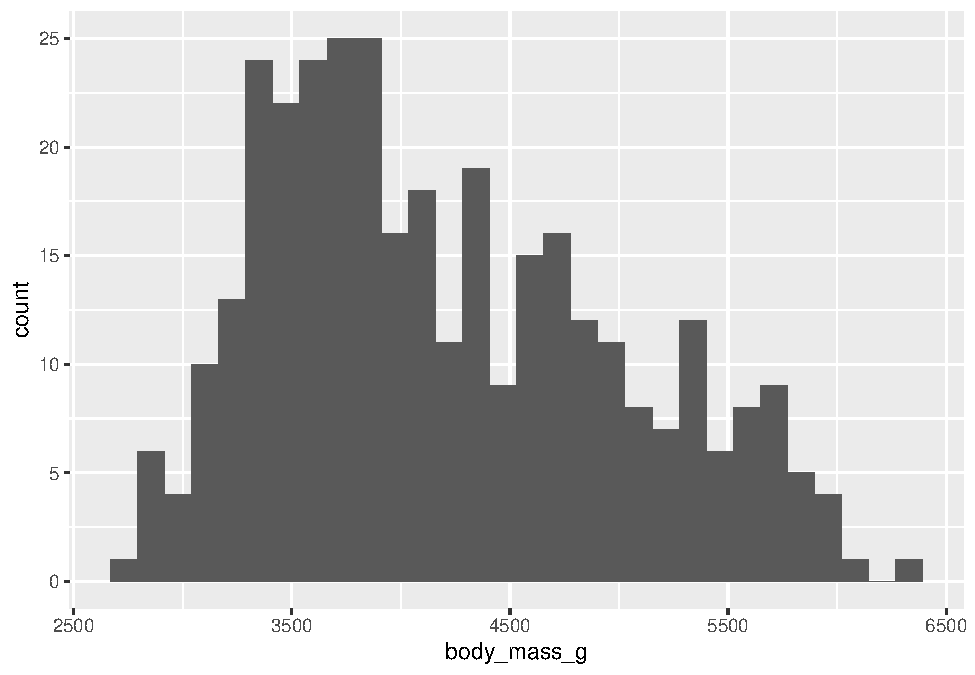
\includegraphics{intro_stats_files/figure-latex/unnamed-chunk-97-1.pdf}

\hypertarget{numerical-shape}{%
\subsection{The shape of data}\label{numerical-shape}}

The way histograms work is to create ``bins'', which are ranges of numbers along the x-axis. R goes through the data and counts how many observations fall into each bin. In that way, a histogram is somewhat like a bar chart. However, a bar chart uses bars to represent distinct, discrete categories, whereas a histogram uses bars that are all next to each other to represent values along a continuous numerical range. Histograms are meant to give you--at a quick glance--a sense of the ``shape'' of the data.

What do we mean by ``shape''? Generally, we look for three things:

\begin{enumerate}
\def\labelenumi{\arabic{enumi}.}
\tightlist
\item
  Modes
\end{enumerate}

\begin{itemize}
\tightlist
\item
  Modes are peaks in the data. These are places where data tends to cluster, representing common values of the numerical variable. In the \texttt{penguin} data, there appears to be a big mode between about 3500 and 4000 grams. When data has one clear mode, we call the data \emph{unimodal}. But data can also be \emph{bimodal}, or more generally, \emph{multimodal}. This often happens when the data contains multiple groups that are different from each other. In this case, we know there are three species of penguin in the data, so if those species are drastically different in their body mass, we might be looking at multimodal data. We'll explore this question more later in the chapter. For now, it's hard to say what's going on because the above histogram has a lot of spiky bars popping up all over. It's not completely obvious how many modes there might be.
\end{itemize}

\begin{enumerate}
\def\labelenumi{\arabic{enumi}.}
\setcounter{enumi}{1}
\tightlist
\item
  Symmetry
\end{enumerate}

\begin{itemize}
\tightlist
\item
  If there is one mode, we can also ask if the data is spread evenly to the left and right of that mode. If so, we call the data \emph{symmetric}. No data is perfectly symmetric, but we are looking for overall balance between the areas to the left and right of the mode. When data is not symmetric, we call is \emph{skewed}. Assuming that there is one big mode around 3500 or 4000, the body mass data above is skewed. There is clearly more data above the mode than below the mode. The right side of the histogram stretches out further to the right of the mode than to the left. Therefore, the body mass data is \emph{right-skewed}. There is a longer ``tail'' to the right. If it were the opposite, it would be \emph{left-skewed}. It is common for beginning students to confuse these two terms. Be aware that we are not concerned about where the mode is. We want to know which side has more data spread into a longer tail. That is the direction of the skewness.
\end{itemize}

\begin{enumerate}
\def\labelenumi{\arabic{enumi}.}
\setcounter{enumi}{2}
\tightlist
\item
  Outliers.
\end{enumerate}

\begin{itemize}
\tightlist
\item
  Outliers are data points that are far from the bulk of the data. The body mass data above appears to have no outliers. We are looking for a large gap between the main ``mass'' of data and any lingering data points far away from that mass. There is no such large gap in the histogram above.
\end{itemize}

\textbf{Whenever you are asked about the ``shape'' of a numerical variable, be sure to comment on (1) modes, (2) symmetry, and (3) outliers.}

Generally, the default binning for \texttt{ggplot} histograms is not great. This is by design. The creator of the \texttt{gglot2} package, Hadley Wickham, said the following:

\begin{quote}
``In ggplot2, a very simple heuristic is used for the default number of bins: it uses 30, regardless of the data. This is perverse, and ignores all of the research on selecting good bin sizes automatically, but sends a clear message to the user that he or she needs to think about, and experiment with, the bin width. This message is reinforced with a warning that reminds the user to manually adjust the bin width.''
\end{quote}

Indeed, if you look at the output from the graphing command above, you can see that \texttt{ggplot} informs you that you should pick a better value for the binwidth. You can also see that the bins aren't ideal. They are too narrow, which means that arbitrary differences between bins show up as ``random'' spikes all over the graph. These spikes can confuse the issue of how many modes appear in the data.

Instead, we should aim to use bins that show the overall shape of the data and smooth it out a bit. Look back at the scale of the x-axis to assess how wide each bar should be. There's no one correct answer. In this case, the bins ought to be a little wider. Since our x-axis goes from about 2500 to 6500, maybe we should try a binwidth of 250. And if 250 doesn't look good, nothing prevents us from trying a different number.

It's also easier to interpret the histogram when the bins' edges line up with numbers that are easy to see in the plot. Use \texttt{boundary} to determine where you want the bin boundaries to fall. For example, if we set the boundary to 3500, that means that one bar will start with its left edge at 3500. This is convenient because there is a tick mark labeled there on the x-axis. The boundary number is pretty arbitrary; once one boundary is set, it determines where all the other bins will line up. With a binwidth of 250, we'd get the same graph if the boundary were set to 3000 or 3250 or 5750, or even 0. Any other multiple of 250 would give the same graph.

We use \texttt{binwidth} and \texttt{boundary} inside the parentheses of the \texttt{geom\_histogram} to modify these parameters.

\begin{Shaded}
\begin{Highlighting}[]
\FunctionTok{ggplot}\NormalTok{(penguins, }\FunctionTok{aes}\NormalTok{(}\AttributeTok{x =}\NormalTok{ body\_mass\_g)) }\SpecialCharTok{+}
    \FunctionTok{geom\_histogram}\NormalTok{(}\AttributeTok{binwidth =} \DecValTok{250}\NormalTok{, }\AttributeTok{boundary =} \DecValTok{3500}\NormalTok{)}
\end{Highlighting}
\end{Shaded}

\begin{verbatim}
## Warning: Removed 2 rows containing non-finite values (stat_bin).
\end{verbatim}

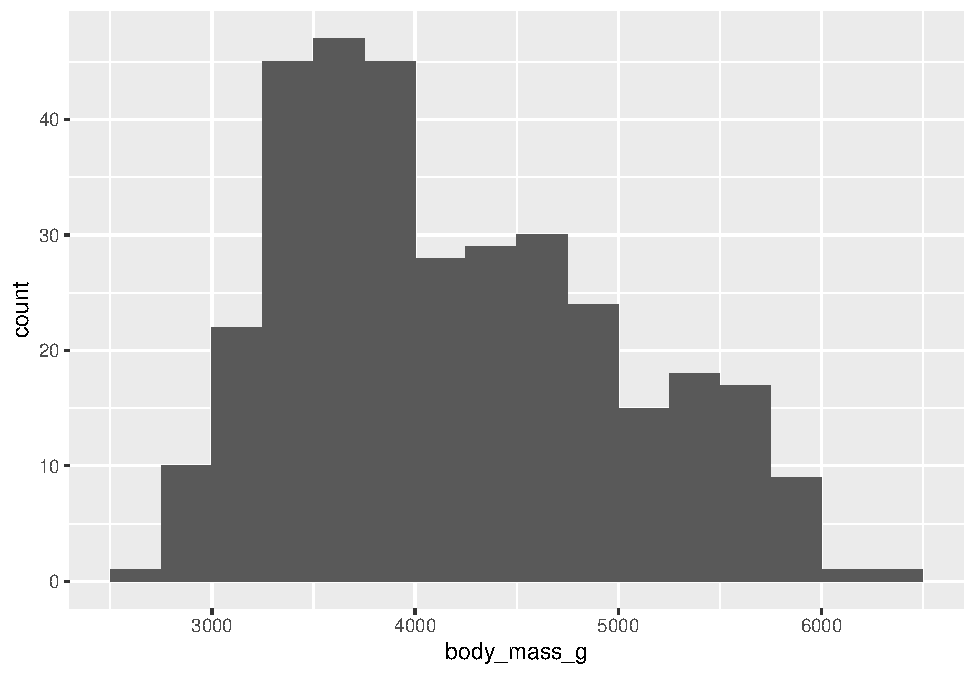
\includegraphics{intro_stats_files/figure-latex/unnamed-chunk-98-1.pdf}

Even with the smoother look, it appears that there are multiple modes, maybe three? Do these correspond to the three species of penguin? Stay tuned.

\hypertarget{exercise-6a-1}{%
\paragraph*{Exercise 6(a)}\label{exercise-6a-1}}
\addcontentsline{toc}{paragraph}{Exercise 6(a)}

Here is a histogram of the penguin bill lengths (measured in millimeters):

\begin{Shaded}
\begin{Highlighting}[]
\FunctionTok{ggplot}\NormalTok{(penguins, }\FunctionTok{aes}\NormalTok{(}\AttributeTok{x =}\NormalTok{ bill\_length\_mm)) }\SpecialCharTok{+}
    \FunctionTok{geom\_histogram}\NormalTok{(}\AttributeTok{binwidth =} \DecValTok{6}\NormalTok{, }\AttributeTok{boundary =} \DecValTok{30}\NormalTok{)}
\end{Highlighting}
\end{Shaded}

\begin{verbatim}
## Warning: Removed 2 rows containing non-finite values (stat_bin).
\end{verbatim}

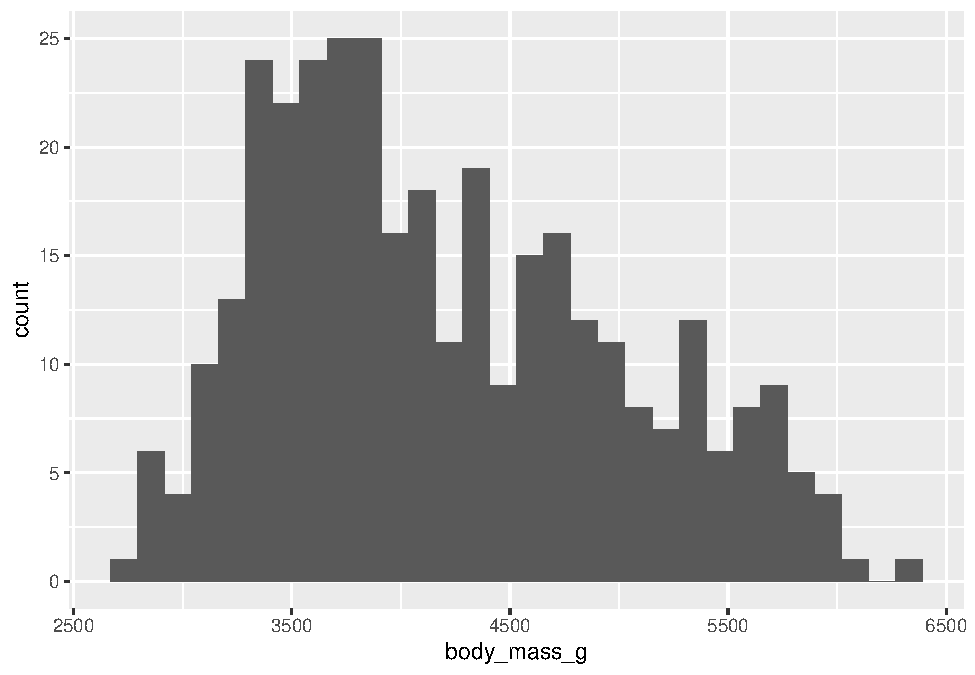
\includegraphics{intro_stats_files/figure-latex/unnamed-chunk-99-1.pdf}

Write a short paragraph describing the shape of the distribution of penguin bill lengths, focusing on the three key shape features (modes, symmetry, and outliers).

Please write up your answer here.

\hypertarget{exercise-6b-1}{%
\paragraph*{Exercise 6(b)}\label{exercise-6b-1}}
\addcontentsline{toc}{paragraph}{Exercise 6(b)}

The last question was a trick question!

Change the binwidth (no need to change the boundary) to something smaller to see more clearly the bimodal nature of the distribution.

\begin{Shaded}
\begin{Highlighting}[]
\CommentTok{\# Add code here that changes the binwidth of the last histogram to see}
\CommentTok{\# the bimodal nature of the distribution.}
\end{Highlighting}
\end{Shaded}

\hypertarget{exercise-7a-1}{%
\paragraph*{Exercise 7(a)}\label{exercise-7a-1}}
\addcontentsline{toc}{paragraph}{Exercise 7(a)}

Make a histogram of the variable \texttt{flipper\_length\_mm}. Start with a histogram where you don't modify the binwidth or boundary.

\begin{Shaded}
\begin{Highlighting}[]
\CommentTok{\# Add code here to create a histogram of flipper length}
\end{Highlighting}
\end{Shaded}

\hypertarget{exercise-7b-1}{%
\paragraph*{Exercise 7(b)}\label{exercise-7b-1}}
\addcontentsline{toc}{paragraph}{Exercise 7(b)}

By examining the scale on the x-axis above, repeat the command, but this time change the binwidth and the boundary until you are satisfied that the bins are neither too wide nor too narrow.

\begin{Shaded}
\begin{Highlighting}[]
\CommentTok{\# Add code here to modify the histogram of flipper length,}
\CommentTok{\# adding binwidth and boundary}
\end{Highlighting}
\end{Shaded}

\hypertarget{exercise-7c-1}{%
\paragraph*{Exercise 7(c)}\label{exercise-7c-1}}
\addcontentsline{toc}{paragraph}{Exercise 7(c)}

Write a short paragraph describing the shape of the distribution of penguin flipper lengths, focusing on the three key shape features (modes, symmetry, and outliers).

Please write up your answer here.

\hypertarget{numerical-less-useful}{%
\subsection{Less useful plot types}\label{numerical-less-useful}}

There are several other graph types that one might see for a single numerical variable: e.g., dotplots, stem-and-leaf plots, boxplots, etc. I'm not a big fan of dotplots or stem-and-leaf plots as they are just messier versions of histograms. I do like boxplots, but they are typically less informative than histograms. Boxplots are much better for comparing groups, and we'll see them later in the chapter.

\hypertarget{numerical-graphing-two}{%
\section{Graphing two numerical variables}\label{numerical-graphing-two}}

The proper graph for two numerical variables is a scatterplot. We graph the response variable on the y-axis and the predictor variable on the x-axis.

Let's consider a possible association between bill length and body mass. For this question, there is not really a strong preference for which variable serves as response and which variable servers as predictor. We'll consider bill length as the response variable and body mass as the predictor.

Since we are plotting two variables, we have two aesthetics, one on the y-axis (the response variable) and one on the x-axis (the predictor variable). Since scatterplots use points to plot each data value, the correct layer to add is \texttt{geom\_point()}.

\begin{Shaded}
\begin{Highlighting}[]
\FunctionTok{ggplot}\NormalTok{(penguins, }\FunctionTok{aes}\NormalTok{(}\AttributeTok{y =}\NormalTok{ bill\_length\_mm, }\AttributeTok{x =}\NormalTok{ body\_mass\_g)) }\SpecialCharTok{+}
    \FunctionTok{geom\_point}\NormalTok{()}
\end{Highlighting}
\end{Shaded}

\begin{verbatim}
## Warning: Removed 2 rows containing missing values (geom_point).
\end{verbatim}

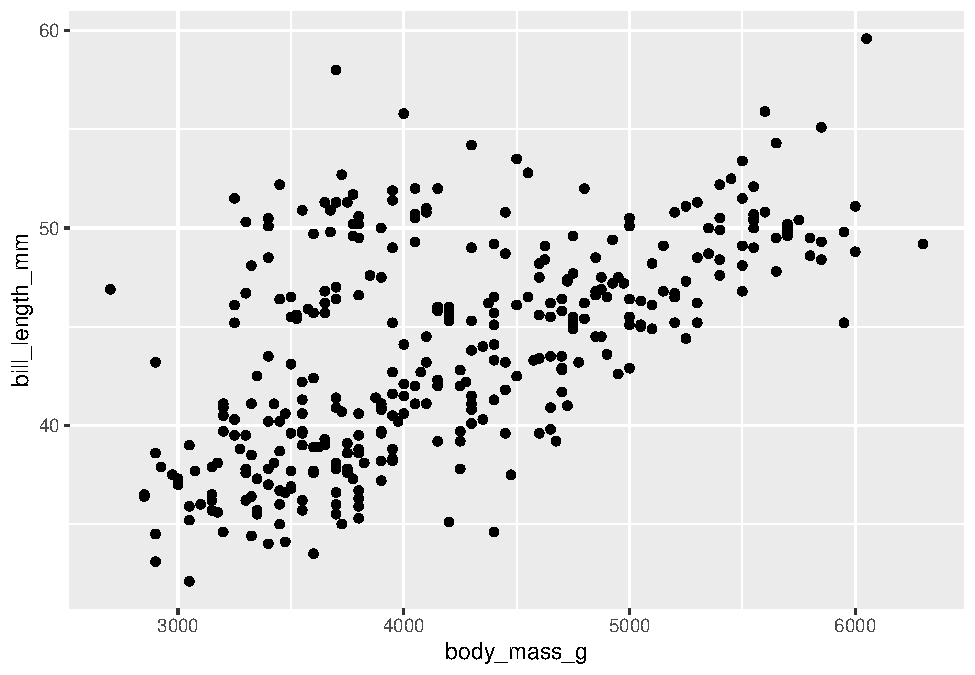
\includegraphics{intro_stats_files/figure-latex/unnamed-chunk-103-1.pdf}

We are looking for evidence of a relationship between the two variables. This will manifest as a pattern in the data. We are interested in answering the following questions:

\begin{enumerate}
\def\labelenumi{\arabic{enumi}.}
\tightlist
\item
  Linearity
\end{enumerate}

\begin{itemize}
\tightlist
\item
  Is the association linear? In other words, do the data points lie roughly in a straight line pattern? The scatterplot above is a bit ``cloudy'' but generally moves from lower left to upper right in a straight (not curved pattern). It's not a completely random scatter of dots.
\end{itemize}

\begin{enumerate}
\def\labelenumi{\arabic{enumi}.}
\setcounter{enumi}{1}
\tightlist
\item
  Direction
\end{enumerate}

\begin{itemize}
\tightlist
\item
  If the pattern is linear, it is a \emph{positive} relationship or a \emph{negative} one? Positive means that the line moves from lower left to upper right. Negative means it moves from upper left to lower right. If you recall the direction of slopes from high school algebra class, a positive association corresponds to a line with a positive slope, and similarly for a negative association. In the data above, lower values of body mass correspond to lower bill lengths, and higher values of body mass correspond to higher bill lengths. So this is a positive association.
\end{itemize}

\begin{enumerate}
\def\labelenumi{\arabic{enumi}.}
\setcounter{enumi}{2}
\tightlist
\item
  Strength
\end{enumerate}

\begin{itemize}
\tightlist
\item
  If there is a pattern, how tight is the pattern? Do the data points stay close to a straight line, or are they pretty spread out and only generally moving in one direction. A strong relationship is one that is tightly packed around a line or curve. The relationship above is not strong. We might use terms like ``weak'', ``moderately weak'', or ``moderate'', but definitely not strong.
\end{itemize}

\begin{enumerate}
\def\labelenumi{\arabic{enumi}.}
\setcounter{enumi}{3}
\tightlist
\item
  Outliers
\end{enumerate}

\begin{itemize}
\tightlist
\item
  Are there outliers? These will be points that are isolated and relatively far from the bulk of the data. There are a few points above that are borderline, but none is a particularly strong outlier, especially give how spread out the rest of the data is.
\end{itemize}

\hypertarget{exercise-8}{%
\paragraph*{Exercise 8}\label{exercise-8}}
\addcontentsline{toc}{paragraph}{Exercise 8}

Here is a scatterplot of

\begin{Shaded}
\begin{Highlighting}[]
\FunctionTok{ggplot}\NormalTok{(penguins, }\FunctionTok{aes}\NormalTok{(}\AttributeTok{y =}\NormalTok{ flipper\_length\_mm, }\AttributeTok{x =}\NormalTok{ body\_mass\_g)) }\SpecialCharTok{+}
    \FunctionTok{geom\_point}\NormalTok{()}
\end{Highlighting}
\end{Shaded}

\begin{verbatim}
## Warning: Removed 2 rows containing missing values (geom_point).
\end{verbatim}

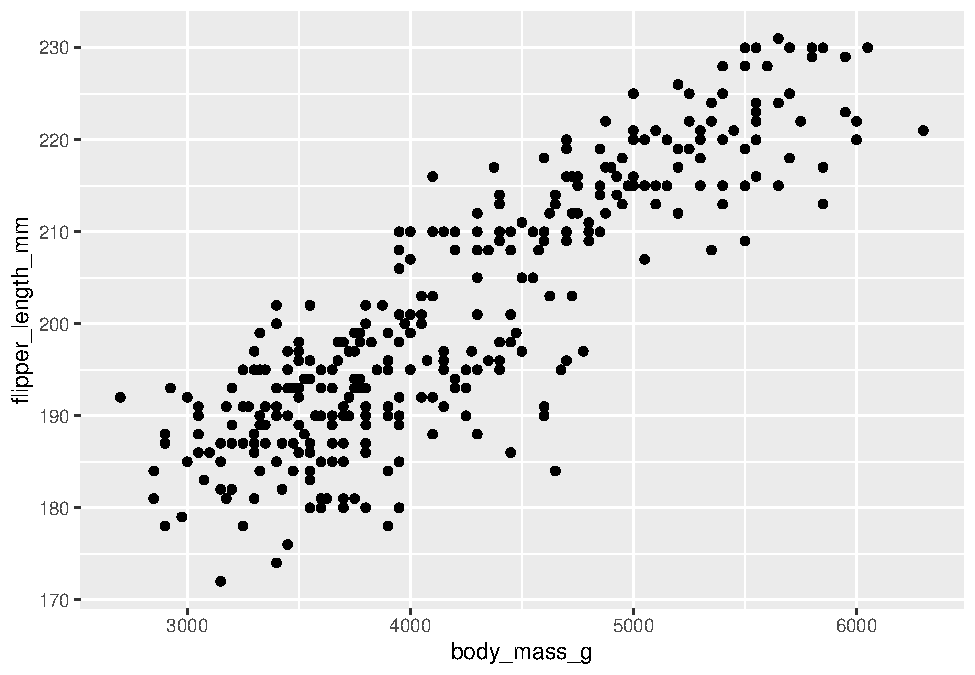
\includegraphics{intro_stats_files/figure-latex/unnamed-chunk-104-1.pdf}

Write a short paragraph describing the association of penguin flipper lengths and body mass, focusing on the four key features (linearity, direction, strength, and outliers).

Please write up your answer here.

\hypertarget{numerical-graphing-grouped}{%
\section{Graphing grouped numerical data}\label{numerical-graphing-grouped}}

Suppose you want to analyze one numerical variable and one categorical variable. Usually, the idea here is that the categorical variable divides up the data into groups and you are interested in understanding the numerical variable for each group separately. Another way to say this is that your numerical variable is response and your categorical variable is predictor. (It is also possible for a categorical variable to be response and a numerical variable to be predictor. This is common in so-called ``classification'' problems. We will not cover this possibility in this course, but it is covered in more advanced courses.)

This turns out to be exactly what we need in the penguins data. Throughout the above exercises, there was a concern that the penguin measurements are fundamentally different among three different species of penguin.

Graphically, there are two good options here. The first is a side-by-side boxplot.

\begin{Shaded}
\begin{Highlighting}[]
\FunctionTok{ggplot}\NormalTok{(penguins, }\FunctionTok{aes}\NormalTok{(}\AttributeTok{y =}\NormalTok{ body\_mass\_g, }\AttributeTok{x =}\NormalTok{ species)) }\SpecialCharTok{+}
    \FunctionTok{geom\_boxplot}\NormalTok{()}
\end{Highlighting}
\end{Shaded}

\begin{verbatim}
## Warning: Removed 2 rows containing non-finite values (stat_boxplot).
\end{verbatim}

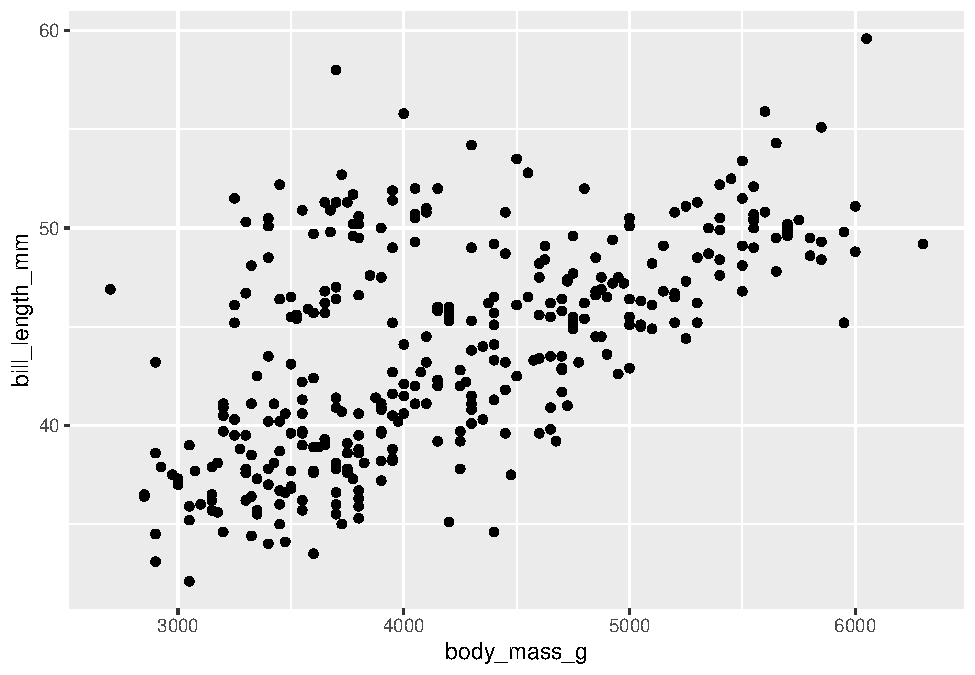
\includegraphics{intro_stats_files/figure-latex/unnamed-chunk-105-1.pdf}

Notice the placement of the variables. The y-axis is \texttt{body\_mass\_g}, the numerical variable. The x-axis variable is \texttt{species}; the groups are placed along the x-axis. This is consistent with other graph types that place the response variable on the y-axis and the predictor variable on the x-axis.

The other possible graph is a stacked histogram. This uses a feature called ``faceting'' that creates a different plot for each group. The syntax is a little unusual.

\begin{Shaded}
\begin{Highlighting}[]
\FunctionTok{ggplot}\NormalTok{(penguins, }\FunctionTok{aes}\NormalTok{(}\AttributeTok{x =}\NormalTok{ body\_mass\_g)) }\SpecialCharTok{+}
    \FunctionTok{geom\_histogram}\NormalTok{() }\SpecialCharTok{+}
    \FunctionTok{facet\_grid}\NormalTok{(species }\SpecialCharTok{\textasciitilde{}}\NormalTok{ .)}
\end{Highlighting}
\end{Shaded}

\begin{verbatim}
## `stat_bin()` using `bins = 30`. Pick better value with `binwidth`.
\end{verbatim}

\begin{verbatim}
## Warning: Removed 2 rows containing non-finite values (stat_bin).
\end{verbatim}

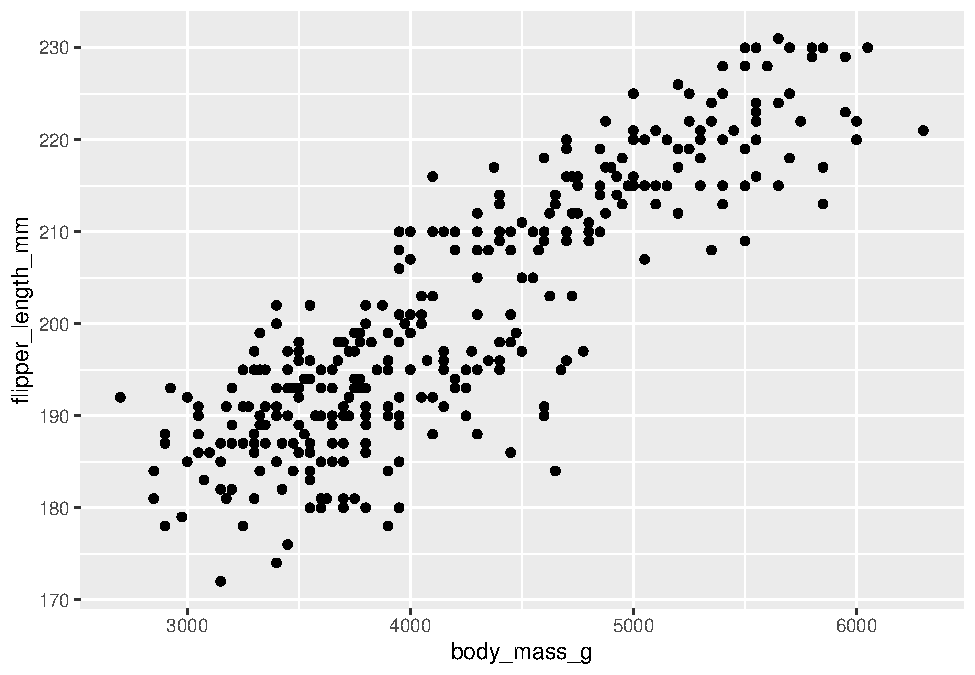
\includegraphics{intro_stats_files/figure-latex/unnamed-chunk-106-1.pdf}

The argument \texttt{species\ \textasciitilde{}\ .} in the \texttt{facet\_grid} function means, ``Put each species on a different row.'' We'll explore this notation a little later.

As always, the default bins suck, so let's change them.

\begin{Shaded}
\begin{Highlighting}[]
\FunctionTok{ggplot}\NormalTok{(penguins, }\FunctionTok{aes}\NormalTok{(}\AttributeTok{x =}\NormalTok{ body\_mass\_g)) }\SpecialCharTok{+}
    \FunctionTok{geom\_histogram}\NormalTok{(}\AttributeTok{binwidth =} \DecValTok{250}\NormalTok{, }\AttributeTok{boundary =} \DecValTok{3500}\NormalTok{) }\SpecialCharTok{+}
    \FunctionTok{facet\_grid}\NormalTok{(species }\SpecialCharTok{\textasciitilde{}}\NormalTok{ .)}
\end{Highlighting}
\end{Shaded}

\begin{verbatim}
## Warning: Removed 2 rows containing non-finite values (stat_bin).
\end{verbatim}

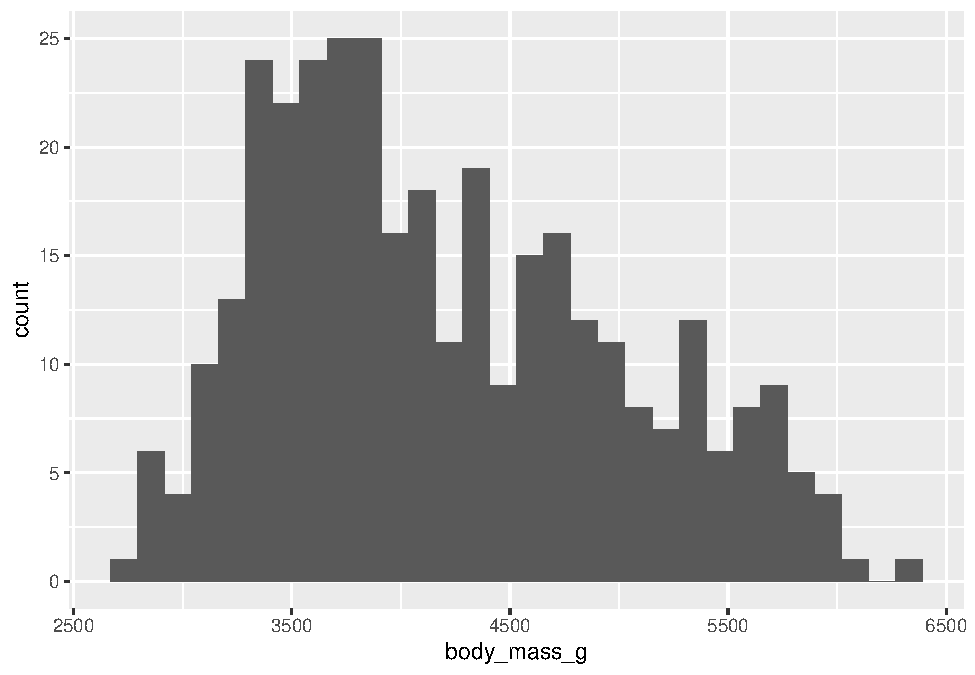
\includegraphics{intro_stats_files/figure-latex/unnamed-chunk-107-1.pdf}

Consider the following subtle change in notation:

\begin{Shaded}
\begin{Highlighting}[]
\FunctionTok{ggplot}\NormalTok{(penguins, }\FunctionTok{aes}\NormalTok{(}\AttributeTok{x =}\NormalTok{ body\_mass\_g)) }\SpecialCharTok{+}
    \FunctionTok{geom\_histogram}\NormalTok{(}\AttributeTok{binwidth =} \DecValTok{250}\NormalTok{, }\AttributeTok{boundary =} \DecValTok{3500}\NormalTok{) }\SpecialCharTok{+}
    \FunctionTok{facet\_grid}\NormalTok{(. }\SpecialCharTok{\textasciitilde{}}\NormalTok{ species)}
\end{Highlighting}
\end{Shaded}

\begin{verbatim}
## Warning: Removed 2 rows containing non-finite values (stat_bin).
\end{verbatim}

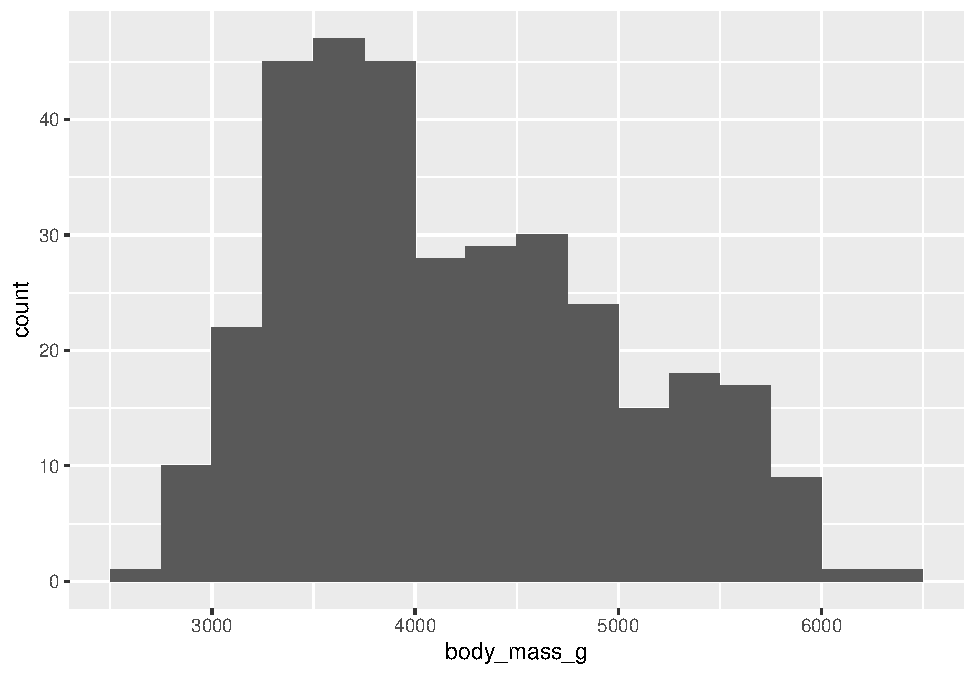
\includegraphics{intro_stats_files/figure-latex/unnamed-chunk-108-1.pdf}

\hypertarget{exercise-9a-1}{%
\paragraph*{Exercise 9(a)}\label{exercise-9a-1}}
\addcontentsline{toc}{paragraph}{Exercise 9(a)}

Explain why that last graph (which might be called a side-by-side histogram) is less effective than the earlier stacked histogram. (Hint: what stays lined up when the histograms are stacked vertically rather than horizontally?)

Please write up your answer here.

\hypertarget{exercise-9b-1}{%
\paragraph*{Exercise 9(b)}\label{exercise-9b-1}}
\addcontentsline{toc}{paragraph}{Exercise 9(b)}

Can you figure out what's going on with the weird syntax of \texttt{species\ \textasciitilde{}\ .} vs \texttt{.\ \textasciitilde{}\ species}? Explain it in your own words.

Please write up your answer here.

\begin{center}\rule{0.5\linewidth}{0.5pt}\end{center}

The other thing that kind of sucks is the fact that the y-axis is showing counts. That makes it harder to see the distribution of body mass among Chinstrap penguins, for example, as there are fewer of them in the data set. It would be nice to scale these using percentages.

\begin{Shaded}
\begin{Highlighting}[]
\FunctionTok{ggplot}\NormalTok{(penguins, }\FunctionTok{aes}\NormalTok{(}\AttributeTok{x =}\NormalTok{ body\_mass\_g)) }\SpecialCharTok{+}
    \FunctionTok{geom\_histogram}\NormalTok{(}\FunctionTok{aes}\NormalTok{(}\AttributeTok{y =}\NormalTok{ ..density..),}
                   \AttributeTok{binwidth =} \DecValTok{250}\NormalTok{, }\AttributeTok{boundary =} \DecValTok{3500}\NormalTok{) }\SpecialCharTok{+}
    \FunctionTok{facet\_grid}\NormalTok{(species }\SpecialCharTok{\textasciitilde{}}\NormalTok{ .)}
\end{Highlighting}
\end{Shaded}

\begin{verbatim}
## Warning: Removed 2 rows containing non-finite values (stat_bin).
\end{verbatim}

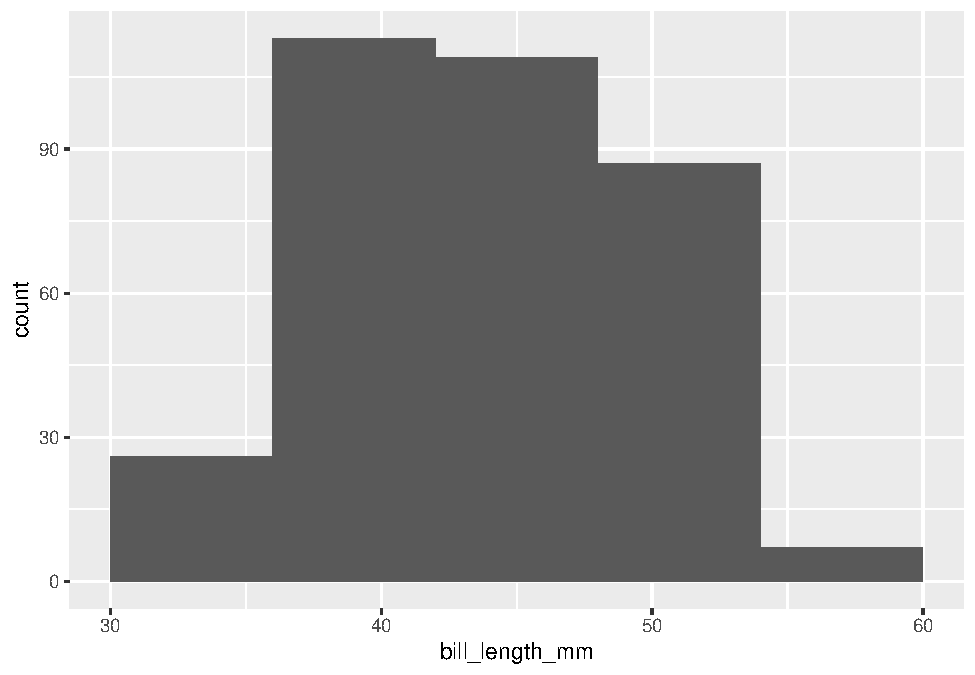
\includegraphics{intro_stats_files/figure-latex/unnamed-chunk-109-1.pdf}

Due to some technical issues in \texttt{ggplot2}, these are not strictly proportions. (If you were to add up the heights of all the bars, they would not add up to 100\%.) Nevertheless, the graph is still useful because it does scale the groups to put them on equal footing. In other words, it treats each group as if they all had the same sample size.

\hypertarget{exercise-10}{%
\paragraph*{Exercise 10}\label{exercise-10}}
\addcontentsline{toc}{paragraph}{Exercise 10}

Choose a numerical variable that's not body mass and a categorical variable that's not species from the \texttt{penguins} data set. Make both a side-by-side boxplot and a stacked histogram. Discuss the resulting graphs. Comment on the association (or independence) of the two variables. If there is an association, be sure to focus on the four key features (linearity, direction, strength, and outliers).

\begin{Shaded}
\begin{Highlighting}[]
\CommentTok{\# Add code here to create a side{-}by{-}side boxplot.}
\end{Highlighting}
\end{Shaded}

\begin{Shaded}
\begin{Highlighting}[]
\CommentTok{\# Add code here to create a stacked histogram.}
\end{Highlighting}
\end{Shaded}

Please write up your answer here.

\hypertarget{numerical-pub}{%
\section{Publication-ready graphics}\label{numerical-pub}}

The great thing about \texttt{ggplot2} graphics is that they are already quite pretty. To take them from exploratory data analysis to the next level, there are a few things we can do to tidy them up.

Let's go back to the first histogram from this chapter.

\begin{Shaded}
\begin{Highlighting}[]
\FunctionTok{ggplot}\NormalTok{(penguins, }\FunctionTok{aes}\NormalTok{(}\AttributeTok{x =}\NormalTok{ body\_mass\_g)) }\SpecialCharTok{+}
    \FunctionTok{geom\_histogram}\NormalTok{(}\AttributeTok{binwidth =} \DecValTok{250}\NormalTok{, }\AttributeTok{boundary =} \DecValTok{3500}\NormalTok{)}
\end{Highlighting}
\end{Shaded}

\begin{verbatim}
## Warning: Removed 2 rows containing non-finite values (stat_bin).
\end{verbatim}

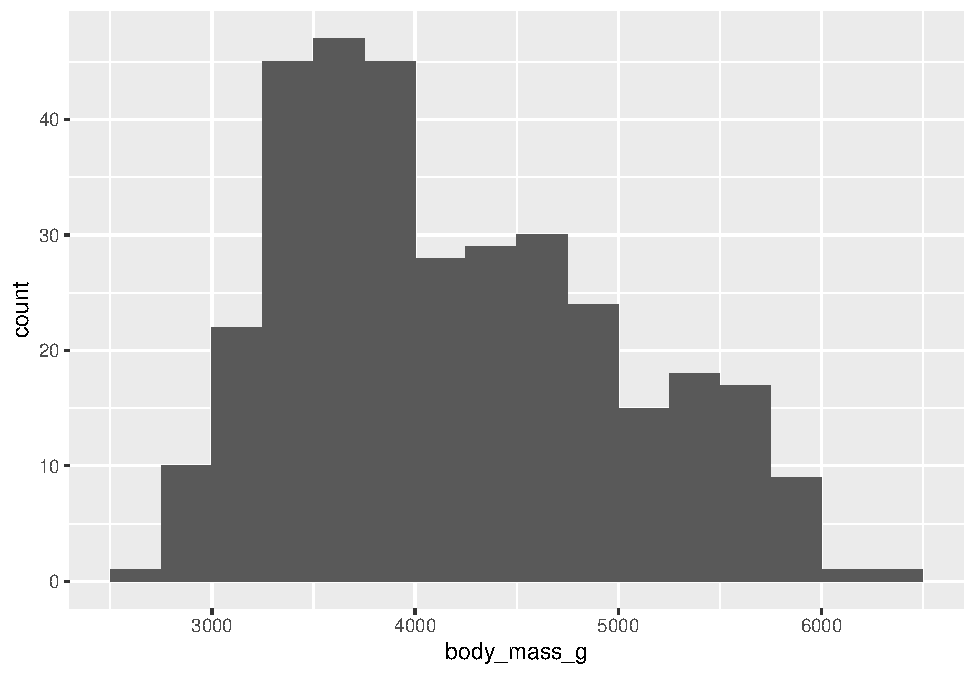
\includegraphics{intro_stats_files/figure-latex/unnamed-chunk-112-1.pdf}

The variable names of this data set are already pretty informative, but we can do a little better with \texttt{labs} (for labels). Observe:

\begin{Shaded}
\begin{Highlighting}[]
\FunctionTok{ggplot}\NormalTok{(penguins, }\FunctionTok{aes}\NormalTok{(}\AttributeTok{x =}\NormalTok{ body\_mass\_g)) }\SpecialCharTok{+}
    \FunctionTok{geom\_histogram}\NormalTok{(}\AttributeTok{binwidth =} \DecValTok{250}\NormalTok{, }\AttributeTok{boundary =} \DecValTok{3500}\NormalTok{) }\SpecialCharTok{+}
    \FunctionTok{labs}\NormalTok{(}\AttributeTok{title =} \StringTok{"Distribution of body mass for adult foraging penguins near}
\StringTok{         Palmer Station, Antarctica"}\NormalTok{,}
         \AttributeTok{x =} \StringTok{"Body mass (in grams)"}\NormalTok{,}
         \AttributeTok{y =} \StringTok{"Count"}\NormalTok{)}
\end{Highlighting}
\end{Shaded}

\begin{verbatim}
## Warning: Removed 2 rows containing non-finite values (stat_bin).
\end{verbatim}

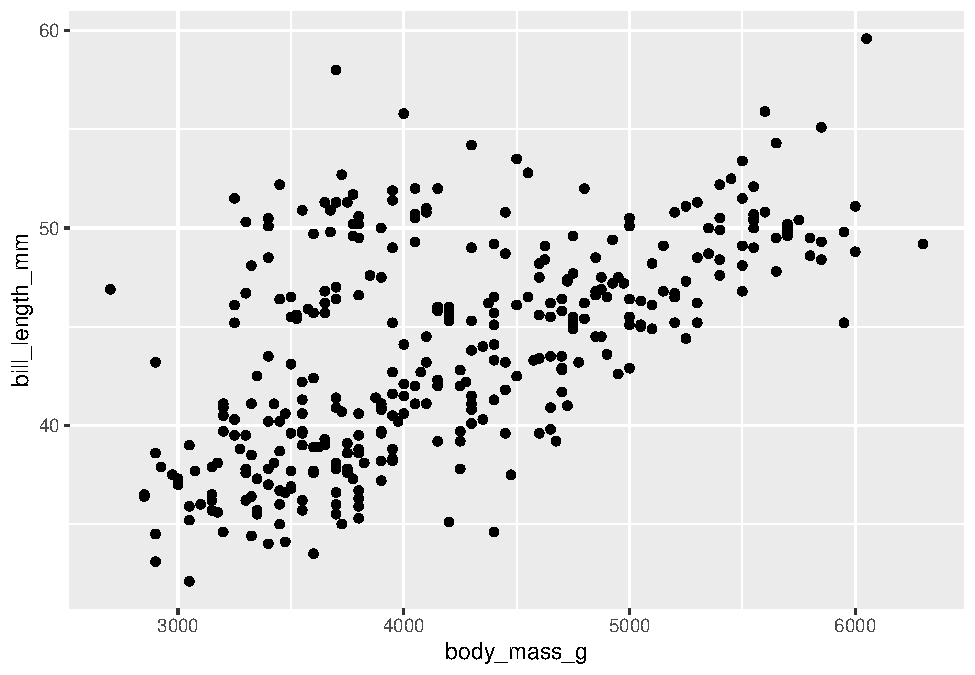
\includegraphics{intro_stats_files/figure-latex/unnamed-chunk-113-1.pdf}

You can also see that we took the opportunity to mention the units of measurement (grams) for our variable in the x-axis label. This is good practice.

A quick note about formatting in R code chunks. Notice that I put different parts of the last \texttt{ggplot} command on their own separate lines. The command would still work if I did this:

\begin{Shaded}
\begin{Highlighting}[]
\FunctionTok{ggplot}\NormalTok{(penguins, }\FunctionTok{aes}\NormalTok{(}\AttributeTok{x =}\NormalTok{ body\_mass\_g)) }\SpecialCharTok{+} \FunctionTok{geom\_histogram}\NormalTok{(}\AttributeTok{binwidth =} \DecValTok{250}\NormalTok{, }\AttributeTok{boundary =} \DecValTok{3500}\NormalTok{) }\SpecialCharTok{+} \FunctionTok{labs}\NormalTok{(}\AttributeTok{title =} \StringTok{"Distribution of body mass for adult foraging penguins near Palmer Station, Antarctica"}\NormalTok{, }\AttributeTok{x =} \StringTok{"Body mass (in grams)"}\NormalTok{, }\AttributeTok{y =} \StringTok{"Count"}\NormalTok{)}
\end{Highlighting}
\end{Shaded}

\begin{verbatim}
## Warning: Removed 2 rows containing non-finite values (stat_bin).
\end{verbatim}

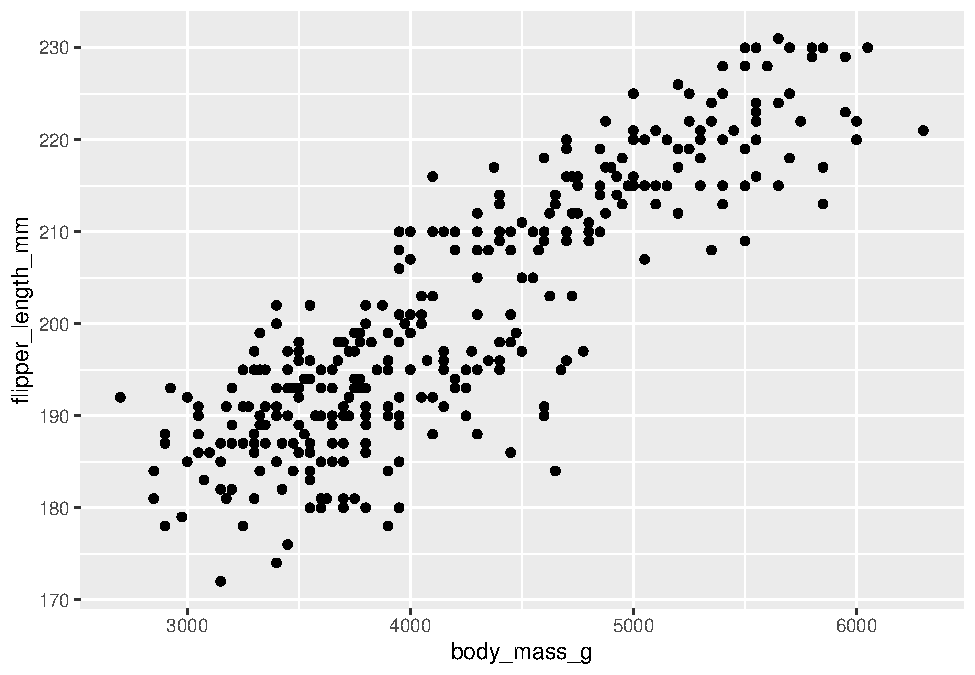
\includegraphics{intro_stats_files/figure-latex/unnamed-chunk-114-1.pdf}

But it's much harder to read. If you find that your code is ``wrapping'' to the next line, find some spots like commas or plus signs to break the code. Be sure to break the line after the comma or plus sign.

\hypertarget{exercise-11-1}{%
\paragraph*{Exercise 11}\label{exercise-11-1}}
\addcontentsline{toc}{paragraph}{Exercise 11}

Modify the following scatterplot by adding a title and labels for both the y-axis and x-axis.

\begin{Shaded}
\begin{Highlighting}[]
\CommentTok{\# Modify the following scatterplot by adding a title and }
\CommentTok{\# labels for both the y{-}axis and x{-}axis.}
\FunctionTok{ggplot}\NormalTok{(penguins, }\FunctionTok{aes}\NormalTok{(}\AttributeTok{y =}\NormalTok{ bill\_length\_mm, }\AttributeTok{x =}\NormalTok{ bill\_depth\_mm)) }\SpecialCharTok{+}
    \FunctionTok{geom\_point}\NormalTok{()}
\end{Highlighting}
\end{Shaded}

\begin{verbatim}
## Warning: Removed 2 rows containing missing values (geom_point).
\end{verbatim}

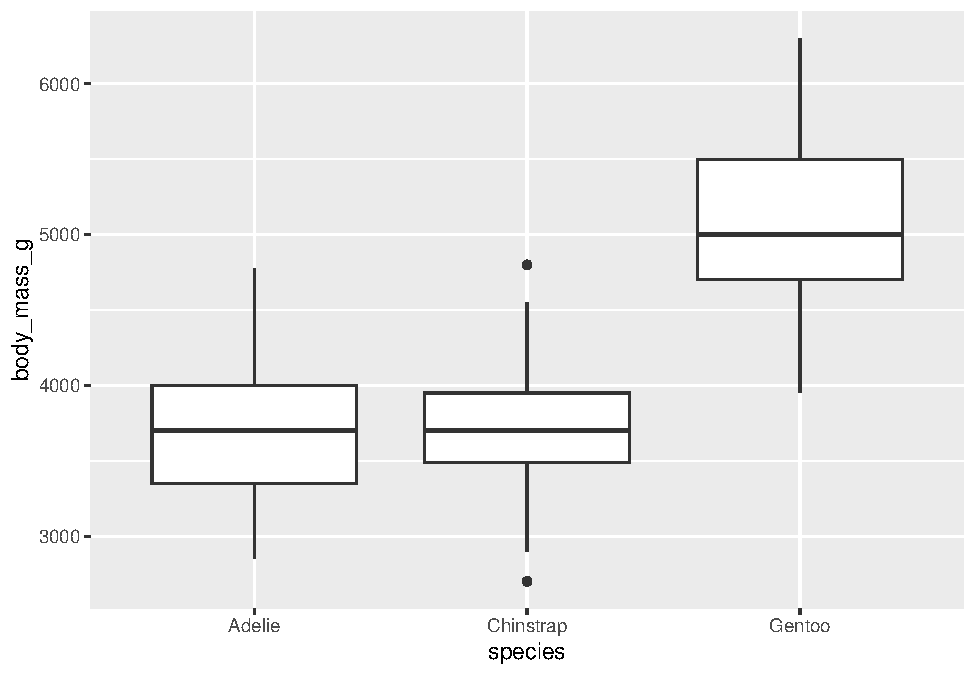
\includegraphics{intro_stats_files/figure-latex/unnamed-chunk-115-1.pdf}

\hypertarget{exercise-12-1}{%
\paragraph*{Exercise 12}\label{exercise-12-1}}
\addcontentsline{toc}{paragraph}{Exercise 12}

The previous scatterplot looked a little funny due to some odd groupings that we suspect (as usual) might be due to multiple species being measures. Add a new aesthetic (so, inside the parentheses following \texttt{aes}) to the following code to assign \texttt{color\ =\ species}. Comment on what you see.

\begin{Shaded}
\begin{Highlighting}[]
\CommentTok{\# Modify the code below to add color = species}
\FunctionTok{ggplot}\NormalTok{(penguins, }\FunctionTok{aes}\NormalTok{(}\AttributeTok{y =}\NormalTok{ bill\_length\_mm, }\AttributeTok{x =}\NormalTok{ bill\_depth\_mm)) }\SpecialCharTok{+}
    \FunctionTok{geom\_point}\NormalTok{()}
\end{Highlighting}
\end{Shaded}

\begin{verbatim}
## Warning: Removed 2 rows containing missing values (geom_point).
\end{verbatim}

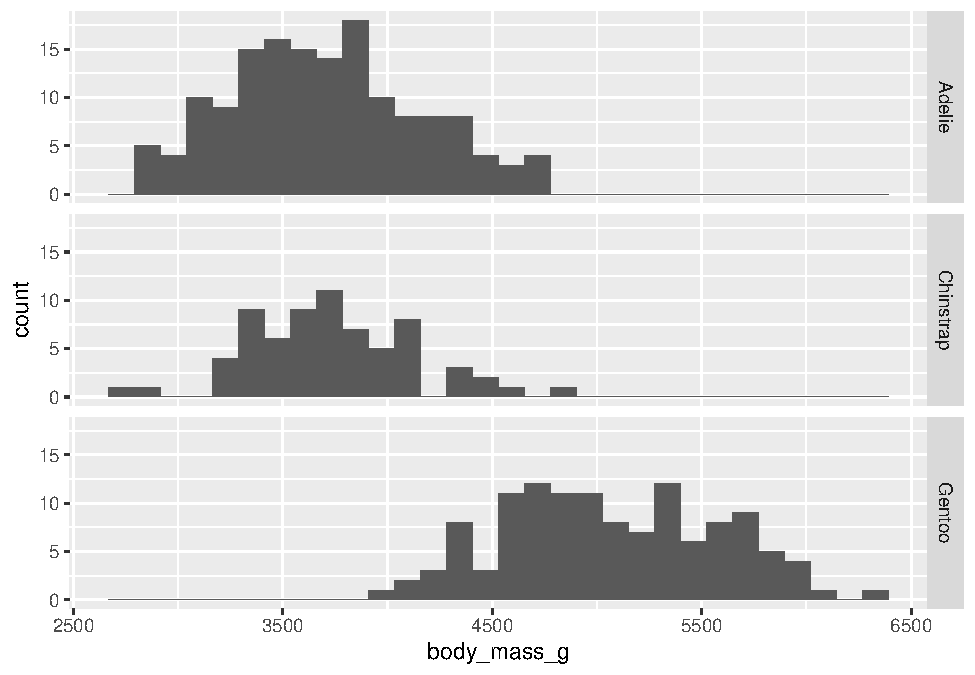
\includegraphics{intro_stats_files/figure-latex/unnamed-chunk-116-1.pdf}

Please write up your answer here.

\begin{center}\rule{0.5\linewidth}{0.5pt}\end{center}

Every part of the graph can be customized, from the color scheme to the tick marks on the axes, to the major and minor grid lines that appear on the background. We won't go into all that, but you can look at the \href{http://ggplot2.tidyverse.org/}{ggplot2 documentation} online and search Google for examples if you want to dig in and figure out how to do some of that stuff. However, the default options are often (but not always) the best, so be careful that your messing around doesn't inadvertently make the graph less clear or less appealing.

\hypertarget{numerical-conclusion}{%
\section{Conclusion}\label{numerical-conclusion}}

Summary statistics are simple numbers that describe and summarize data sets. Measures of center tell us where the ``middle'' of our numerical data lies, and measures of spread tell us how spread out our numerical data is. These measures should always be reported in pairs, for example the mean/standard deviation, or the median/IQR.

The \texttt{ggplot2} package with its \texttt{ggplot} command is a very versatile tool for creating nice graphs relatively easily. For a single numerical variable, the standard graph type is a histogram. For two numerical variables, use a scatterplot. For a numerical response with a categorical predictor, use either a side-by-side boxplot or a stacked histogram.

\hypertarget{numerical-prep}{%
\subsection{Preparing and submitting your assignment}\label{numerical-prep}}

\begin{enumerate}
\def\labelenumi{\arabic{enumi}.}
\tightlist
\item
  From the ``Run'' menu, select ``Restart R and Run All Chunks''.
\item
  Deal with any code errors that crop up. Repeat steps 1---2 until there are no more code errors.
\item
  Spell check your document by clicking the icon with ``ABC'' and a check mark.
\item
  Hit the ``Preview'' button one last time to generate the final draft of the \texttt{.nb.html} file.
\item
  Proofread the HTML file carefully. If there are errors, go back and fix them, then repeat steps 1--5 again.
\end{enumerate}

If you have completed this chapter as part of a statistics course, follow the directions you receive from your professor to submit your assignment.

\hypertarget{manipulating}{%
\chapter{Manipulating data}\label{manipulating}}

2.0

\hypertarget{functions-introduced-in-this-chapter-4}{%
\subsection*{Functions introduced in this chapter}\label{functions-introduced-in-this-chapter-4}}
\addcontentsline{toc}{subsection}{Functions introduced in this chapter}

\texttt{read\_csv}, \texttt{select}, \texttt{rename}, \texttt{rm}, \texttt{filter}, \texttt{slice}, \texttt{arrange}, \texttt{mutate}, \texttt{all.equal}, \texttt{ifelse}, \texttt{transmute}, \texttt{summarise}, \texttt{group\_by}, \texttt{\%\textgreater{}\%}, \texttt{count}

\hypertarget{manipulating-intro}{%
\section{Introduction}\label{manipulating-intro}}

This tutorial will import some data from the web and then explore it using the amazing \texttt{dplyr} package, a package which is quickly becoming the \emph{de facto} standard among R users for manipulating data. It's part of the \texttt{tidyverse} that we've already used in several chapters.

\hypertarget{manipulating-install}{%
\subsection{Install new packages}\label{manipulating-install}}

There are no new packages used in this chapter.

\hypertarget{manipulating-download}{%
\subsection{Download the R notebook file}\label{manipulating-download}}

Check the upper-right corner in RStudio to make sure you're in your \texttt{intro\_stats} project. Then click on the following link to download this chapter as an R notebook file (\texttt{.Rmd}).

https://vectorposse.github.io/intro\_stats/chapter\_downloads/05-manipulating\_data.Rmd

Once the file is downloaded, move it to your project folder in RStudio and open it there.

\hypertarget{manipulating-restart}{%
\subsection{Restart R and run all chunks}\label{manipulating-restart}}

In RStudio, select ``Restart R and Run All Chunks'' from the ``Run'' menu.

\hypertarget{manipulating-load}{%
\subsection{Load packages}\label{manipulating-load}}

We load the \texttt{tidyverse} package as usual, but this time it is to give us access to the \texttt{dplyr} package, which is loaded alongside our other \texttt{tidyverse} packages like \texttt{ggplot2}. The \texttt{tidyverse} also has a package called \texttt{readr} that will allow us to import data from an external source (in this case, a web site).

\begin{Shaded}
\begin{Highlighting}[]
\FunctionTok{library}\NormalTok{(tidyverse)}
\end{Highlighting}
\end{Shaded}

\hypertarget{manipulating-csv}{%
\section{Importing CSV data}\label{manipulating-csv}}

For most of the chapters, we use data sets that are either included in base R or included in a package that can be loaded into R. But it is useful to see how to get a data set from outside the R ecosystem. This depends a lot on the format of the data file, but a common format is a ``comma-separated values'' file, or CSV file. If you have a data set that is not formatted as a CSV file, it is usually pretty easy to open it in something like Google Spreadsheets or Microsoft Excel and then re-save it as a CSV file.

The file we'll import is a random sample from all the commercial domestic flights that departed from Houston, Texas, in 2011.

We use the \texttt{read\_csv} command to import a CSV file. In this case, we're grabbing the file from a web page where the file is hosted. If you have a file on your computer, you can also put the file into your project directory and import it from there. Put the URL (for a web page) or the filename (for a file in your project directory) in quotes inside the \texttt{read\_csv}command. We also need to assign the output to a tibble, so we've called it \texttt{hf} for ``Houston flights''.

\begin{Shaded}
\begin{Highlighting}[]
\NormalTok{hf }\OtherTok{\textless{}{-}} \FunctionTok{read\_csv}\NormalTok{(}\StringTok{"https://vectorposse.github.io/intro\_stats/data/hf.csv"}\NormalTok{)}
\end{Highlighting}
\end{Shaded}

\begin{verbatim}
## Rows: 22758 Columns: 21
## -- Column specification --------------------------------------------------------
## Delimiter: ","
## chr  (5): UniqueCarrier, TailNum, Origin, Dest, CancellationCode
## dbl (16): Year, Month, DayofMonth, DayOfWeek, DepTime, ArrTime, FlightNum, A...
## 
## i Use `spec()` to retrieve the full column specification for this data.
## i Specify the column types or set `show_col_types = FALSE` to quiet this message.
\end{verbatim}

\begin{Shaded}
\begin{Highlighting}[]
\NormalTok{hf}
\end{Highlighting}
\end{Shaded}

\begin{verbatim}
## # A tibble: 22,758 x 21
##     Year Month DayofMonth DayOfWeek DepTime ArrTime UniqueCarrier FlightNum
##    <dbl> <dbl>      <dbl>     <dbl>   <dbl>   <dbl> <chr>             <dbl>
##  1  2011     1         12         3    1419    1515 AA                  428
##  2  2011     1         17         1    1530    1634 AA                  428
##  3  2011     1         24         1    1356    1513 AA                  428
##  4  2011     1          9         7     714     829 AA                  460
##  5  2011     1         18         2     721     827 AA                  460
##  6  2011     1         22         6     717     829 AA                  460
##  7  2011     1         11         2    1953    2051 AA                  533
##  8  2011     1         14         5    2119    2229 AA                  533
##  9  2011     1         26         3    2009    2103 AA                  533
## 10  2011     1         14         5    1629    1734 AA                 1121
## # ... with 22,748 more rows, and 13 more variables: TailNum <chr>,
## #   ActualElapsedTime <dbl>, AirTime <dbl>, ArrDelay <dbl>, DepDelay <dbl>,
## #   Origin <chr>, Dest <chr>, Distance <dbl>, TaxiIn <dbl>, TaxiOut <dbl>,
## #   Cancelled <dbl>, CancellationCode <chr>, Diverted <dbl>
\end{verbatim}

\begin{Shaded}
\begin{Highlighting}[]
\FunctionTok{glimpse}\NormalTok{(hf)}
\end{Highlighting}
\end{Shaded}

\begin{verbatim}
## Rows: 22,758
## Columns: 21
## $ Year              <dbl> 2011, 2011, 2011, 2011, 2011, 2011, 2011, 2011, 2011~
## $ Month             <dbl> 1, 1, 1, 1, 1, 1, 1, 1, 1, 1, 1, 1, 1, 1, 1, 1, 1, 1~
## $ DayofMonth        <dbl> 12, 17, 24, 9, 18, 22, 11, 14, 26, 14, 18, 20, 3, 12~
## $ DayOfWeek         <dbl> 3, 1, 1, 7, 2, 6, 2, 5, 3, 5, 2, 4, 1, 3, 6, 4, 1, 3~
## $ DepTime           <dbl> 1419, 1530, 1356, 714, 721, 717, 1953, 2119, 2009, 1~
## $ ArrTime           <dbl> 1515, 1634, 1513, 829, 827, 829, 2051, 2229, 2103, 1~
## $ UniqueCarrier     <chr> "AA", "AA", "AA", "AA", "AA", "AA", "AA", "AA", "AA"~
## $ FlightNum         <dbl> 428, 428, 428, 460, 460, 460, 533, 533, 533, 1121, 1~
## $ TailNum           <chr> "N577AA", "N518AA", "N531AA", "N586AA", "N558AA", "N~
## $ ActualElapsedTime <dbl> 56, 64, 77, 75, 66, 72, 58, 70, 54, 65, 135, 144, 64~
## $ AirTime           <dbl> 41, 48, 43, 51, 46, 47, 44, 45, 39, 47, 114, 111, 46~
## $ ArrDelay          <dbl> 5, 84, 3, -6, -8, -6, -29, 69, -17, -11, 39, -1, -2,~
## $ DepDelay          <dbl> 19, 90, -4, -6, 1, -3, -12, 74, 4, -1, 44, -5, -1, 1~
## $ Origin            <chr> "IAH", "IAH", "IAH", "IAH", "IAH", "IAH", "IAH", "IA~
## $ Dest              <chr> "DFW", "DFW", "DFW", "DFW", "DFW", "DFW", "DFW", "DF~
## $ Distance          <dbl> 224, 224, 224, 224, 224, 224, 224, 224, 224, 224, 96~
## $ TaxiIn            <dbl> 4, 8, 6, 11, 7, 18, 3, 5, 9, 8, 7, 20, 5, 8, 8, 7, 4~
## $ TaxiOut           <dbl> 11, 8, 28, 13, 13, 7, 11, 20, 6, 10, 14, 13, 13, 10,~
## $ Cancelled         <dbl> 0, 0, 0, 0, 0, 0, 0, 0, 0, 0, 0, 0, 0, 0, 0, 0, 0, 0~
## $ CancellationCode  <chr> NA, NA, NA, NA, NA, NA, NA, NA, NA, NA, NA, NA, NA, ~
## $ Diverted          <dbl> 0, 0, 0, 0, 0, 0, 0, 0, 0, 0, 0, 0, 0, 0, 0, 0, 0, 0~
\end{verbatim}

The one disadvantage of a file imported from the internet or your computer is that it does not come with a help file. (Only packages in R have help files.) Hopefully you have access to some kind of information about the data you're importing. In this case, we get lucky because the full Houston flights data set happens to be available in a package called \texttt{hflights}.

\hypertarget{exercise-1-2}{%
\paragraph*{Exercise 1}\label{exercise-1-2}}
\addcontentsline{toc}{paragraph}{Exercise 1}

Go to the help tab in RStudio and search for \texttt{hflights}. Of the several options that appear, click the one from the \texttt{hflights} package (listed as \texttt{hflights::hflights}). Review the help file so you know what all the variables mean. Report below how many cases are in the original \texttt{hflights} data. What fraction of the original data has been sampled in the CSV file we imported above?

Please write up your answer here.

\hypertarget{manipulating-dplyr}{%
\section{\texorpdfstring{Introduction to \texttt{dplyr}}{Introduction to dplyr}}\label{manipulating-dplyr}}

The \texttt{dplyr} package (pronounced ``dee-ply-er'') contains tools for manipulating the rows and columns of tibbles. The key to using \texttt{dplyr} is to familiarize yourself with the ``key verbs'':

\begin{itemize}
\tightlist
\item
  \texttt{select} (and \texttt{rename})
\item
  \texttt{filter} (and \texttt{slice})
\item
  \texttt{arrange}
\item
  \texttt{mutate} (and \texttt{transmute})
\item
  \texttt{summarise} (with \texttt{group\_by})
\end{itemize}

We'll consider these one by one. We won't have time to cover every aspect of these functions. More information appears in the help files, as well as this very helpful ``cheat sheet'': \url{https://raw.githubusercontent.com/rstudio/cheatsheets/main/data-transformation.pdf}

\hypertarget{manipulating-select}{%
\section{\texorpdfstring{\texttt{select}}{select}}\label{manipulating-select}}

The \texttt{select} verb is very easy. It just selects some subset of variables (the columns of your data set).

The \texttt{select} command from the \texttt{dplyr} package illustrates one of the common issues R users face. Because the word ``select'' is pretty common, and selecting things is a common task, there are multiple packages that have a function called \texttt{select}. Depending on the order in which packages were loaded, R might get confused as to which version of \texttt{select} you want and try to apply the wrong one. One way to get the correct version is to specify the package in the syntax. Instead of typing \texttt{select}, we can type \texttt{dplyr::select} to ensure we get the version from the \texttt{dplyr} package. We'll do this in all future uses of the \texttt{select} function. (The other functions in this chapter don't cause us trouble because we don't use any other packages whose functions conflict like this.)

Suppose all we wanted to see was the carrier, origin, and destination. We would type

\begin{Shaded}
\begin{Highlighting}[]
\NormalTok{hf\_select }\OtherTok{\textless{}{-}}\NormalTok{ dplyr}\SpecialCharTok{::}\FunctionTok{select}\NormalTok{(hf, UniqueCarrier, Origin, Dest)}
\NormalTok{hf\_select}
\end{Highlighting}
\end{Shaded}

\begin{verbatim}
## # A tibble: 22,758 x 3
##    UniqueCarrier Origin Dest 
##    <chr>         <chr>  <chr>
##  1 AA            IAH    DFW  
##  2 AA            IAH    DFW  
##  3 AA            IAH    DFW  
##  4 AA            IAH    DFW  
##  5 AA            IAH    DFW  
##  6 AA            IAH    DFW  
##  7 AA            IAH    DFW  
##  8 AA            IAH    DFW  
##  9 AA            IAH    DFW  
## 10 AA            IAH    DFW  
## # ... with 22,748 more rows
\end{verbatim}

A brief but important aside here: there is nothing special about the variable name \texttt{hf\_select}. I could have typed

\texttt{beef\_gravy\ \textless{}-\ dplyr::select(hf,\ UniqueCarrier,\ Origin,\ Dest)}

and it would work just as well. Generally speaking, though, you want to give variables a name that reflects the intent of your analysis.

Also, \textbf{it is important to assign the result to a new variable}. If I had typed

\texttt{hf\ \textless{}-\ dplyr::select(hf,\ UniqueCarrier,\ Origin,\ Dest)}

this would have overwritten the original tibble \texttt{hf} with this new version with only three variables. I want to preserve \texttt{hf} because I want to do other things with the entire data set later. The take-home message here is this: \textbf{Major modifications to your data should generally be given a new variable name.} There are caveats here, though. Every time you create a new variable, you also fill up more memory with your creation. If you check your Global Environment, you'll see that both \texttt{hf} and \texttt{hf\_select} are sitting in there. We'll have more to say about this in a moment.

Okay, back to the \texttt{select} function. The first argument of \texttt{select} is the tibble. After that, just list all the names of the variables you want to select.

If you don't like the names of the variables, you can change them as part of the select process.

\begin{Shaded}
\begin{Highlighting}[]
\NormalTok{hf\_select }\OtherTok{\textless{}{-}}\NormalTok{ dplyr}\SpecialCharTok{::}\FunctionTok{select}\NormalTok{(hf,}
                           \AttributeTok{carrier =}\NormalTok{ UniqueCarrier,}
                           \AttributeTok{origin =}\NormalTok{ Origin,}
                           \AttributeTok{dest =}\NormalTok{ Dest)}
\NormalTok{hf\_select}
\end{Highlighting}
\end{Shaded}

\begin{verbatim}
## # A tibble: 22,758 x 3
##    carrier origin dest 
##    <chr>   <chr>  <chr>
##  1 AA      IAH    DFW  
##  2 AA      IAH    DFW  
##  3 AA      IAH    DFW  
##  4 AA      IAH    DFW  
##  5 AA      IAH    DFW  
##  6 AA      IAH    DFW  
##  7 AA      IAH    DFW  
##  8 AA      IAH    DFW  
##  9 AA      IAH    DFW  
## 10 AA      IAH    DFW  
## # ... with 22,748 more rows
\end{verbatim}

(Note here that I am overwriting \texttt{hf\_select} which had been defined slightly differently before. However, these two versions of \texttt{hf\_select} are basically the same object, so no need to keep two copies here.)

There are a few notational shortcuts. For example, see what the following do.

\begin{Shaded}
\begin{Highlighting}[]
\NormalTok{hf\_select2 }\OtherTok{\textless{}{-}}\NormalTok{ dplyr}\SpecialCharTok{::}\FunctionTok{select}\NormalTok{(hf, DayOfWeek}\SpecialCharTok{:}\NormalTok{UniqueCarrier)}
\NormalTok{hf\_select2}
\end{Highlighting}
\end{Shaded}

\begin{verbatim}
## # A tibble: 22,758 x 4
##    DayOfWeek DepTime ArrTime UniqueCarrier
##        <dbl>   <dbl>   <dbl> <chr>        
##  1         3    1419    1515 AA           
##  2         1    1530    1634 AA           
##  3         1    1356    1513 AA           
##  4         7     714     829 AA           
##  5         2     721     827 AA           
##  6         6     717     829 AA           
##  7         2    1953    2051 AA           
##  8         5    2119    2229 AA           
##  9         3    2009    2103 AA           
## 10         5    1629    1734 AA           
## # ... with 22,748 more rows
\end{verbatim}

\begin{Shaded}
\begin{Highlighting}[]
\NormalTok{hf\_select3 }\OtherTok{\textless{}{-}}\NormalTok{ dplyr}\SpecialCharTok{::}\FunctionTok{select}\NormalTok{(hf, }\FunctionTok{starts\_with}\NormalTok{(}\StringTok{"Taxi"}\NormalTok{))}
\NormalTok{hf\_select3}
\end{Highlighting}
\end{Shaded}

\begin{verbatim}
## # A tibble: 22,758 x 2
##    TaxiIn TaxiOut
##     <dbl>   <dbl>
##  1      4      11
##  2      8       8
##  3      6      28
##  4     11      13
##  5      7      13
##  6     18       7
##  7      3      11
##  8      5      20
##  9      9       6
## 10      8      10
## # ... with 22,748 more rows
\end{verbatim}

\hypertarget{exercise-2-1}{%
\paragraph*{Exercise 2}\label{exercise-2-1}}
\addcontentsline{toc}{paragraph}{Exercise 2}

What is contained in the new tibbles \texttt{hf\_select2} and \texttt{hf\_select3}? In other words, what does the colon (:) appear to do and what does \texttt{starts\_with} appear to do in the \texttt{select} function?

Please write up your answer here.

\begin{center}\rule{0.5\linewidth}{0.5pt}\end{center}

The cheat sheet shows a lot more of these ``helper functions'' if you're interested.

The other command that's related to \texttt{select} is \texttt{rename}. The only difference is that \texttt{select} will throw away any columns you don't select (which is what you want and expect, typically), whereas \texttt{rename} will keep all the columns, but rename those you designate.

\hypertarget{exercise-3-1}{%
\paragraph*{Exercise 3}\label{exercise-3-1}}
\addcontentsline{toc}{paragraph}{Exercise 3}

Putting a minus sign in front of a variable name in the \texttt{select} command will remove the variable. Create a tibble called \texttt{hf\_select4} that removes \texttt{Year}, \texttt{DayofMonth}, \texttt{DayOfWeek}, \texttt{FlightNum}, and \texttt{Diverted}. (Be careful with the unusual---and inconsistent!---capitalization in those variable names.) In the second part of the code chunk below, type \texttt{hf\_select4} so that the tibble prints to the screen (just like in all the above examples).

\begin{Shaded}
\begin{Highlighting}[]
\CommentTok{\# Add code here to define hf\_select4.}
\CommentTok{\# Add code here to print hf\_select4.}
\end{Highlighting}
\end{Shaded}

\hypertarget{manipulating-rm}{%
\section{\texorpdfstring{The \texttt{rm} command}{The rm command}}\label{manipulating-rm}}

Recall that earlier we mentioned the pros and cons of creating a new tibble every time we make a change. On one hand, making a new tibble instead of overwriting the original one will keep the original one available so that we can run different commands on it. On the other hand, making a new tibble does eat up a lot of memory.

One way to get rid of an object once we are done with it is the \texttt{rm} command, where \texttt{rm} is short for ``remove''. When you run the code chunk below, you'll see that all the tibbles we created with \texttt{select} will disappear from your Global Environment.

\begin{Shaded}
\begin{Highlighting}[]
\FunctionTok{rm}\NormalTok{(hf\_select, hf\_select2, hf\_select3)}
\end{Highlighting}
\end{Shaded}

If you need one these tibbles back later, you can always go back and re-run the code chunk that defined it.

We'll use \texttt{rm} at the end of some of the following sections so that we don't use up too much memory.

\hypertarget{exercise-4-2}{%
\paragraph*{Exercise 4}\label{exercise-4-2}}
\addcontentsline{toc}{paragraph}{Exercise 4}

Remove \texttt{hf\_select4} (that you created in Exercise 3) from the Global Environment.

\begin{Shaded}
\begin{Highlighting}[]
\CommentTok{\# Add code here to remove hf\_select4.}
\end{Highlighting}
\end{Shaded}

\hypertarget{manipulating-filter}{%
\section{\texorpdfstring{\texttt{filter}}{filter}}\label{manipulating-filter}}

The \texttt{filter} verb works a lot like \texttt{select}, but for rows instead of columns.

For example, let's say we only want to see Delta flights. We use \texttt{filter}:

\begin{Shaded}
\begin{Highlighting}[]
\NormalTok{hf\_filter }\OtherTok{\textless{}{-}} \FunctionTok{filter}\NormalTok{(hf, UniqueCarrier }\SpecialCharTok{==} \StringTok{"DL"}\NormalTok{)}
\NormalTok{hf\_filter}
\end{Highlighting}
\end{Shaded}

\begin{verbatim}
## # A tibble: 265 x 21
##     Year Month DayofMonth DayOfWeek DepTime ArrTime UniqueCarrier FlightNum
##    <dbl> <dbl>      <dbl>     <dbl>   <dbl>   <dbl> <chr>             <dbl>
##  1  2011     1          4         2    1834    2134 DL                   54
##  2  2011     1          5         3    1606    1903 DL                    8
##  3  2011     1          5         3     543     834 DL                 1248
##  4  2011     1          7         5    1603    1902 DL                    8
##  5  2011     1          7         5    1245    1539 DL                 1204
##  6  2011     1          7         5     933    1225 DL                 1590
##  7  2011     1          8         6     921    1210 DL                 1590
##  8  2011     1         12         3      NA      NA DL                 1590
##  9  2011     1         13         4     928    1224 DL                 1590
## 10  2011     1         13         4     656     947 DL                 1900
## # ... with 255 more rows, and 13 more variables: TailNum <chr>,
## #   ActualElapsedTime <dbl>, AirTime <dbl>, ArrDelay <dbl>, DepDelay <dbl>,
## #   Origin <chr>, Dest <chr>, Distance <dbl>, TaxiIn <dbl>, TaxiOut <dbl>,
## #   Cancelled <dbl>, CancellationCode <chr>, Diverted <dbl>
\end{verbatim}

In the printout of the tibble above, if you can't see the \texttt{UniqueCarrier} column, click the black arrow on the right to scroll through the columns until you can see it. You can click ``Next'' at the bottom to scroll through the rows.

\hypertarget{exercise-5-2}{%
\paragraph*{Exercise 5}\label{exercise-5-2}}
\addcontentsline{toc}{paragraph}{Exercise 5}

How many rows did we get in the \texttt{hf\_filter} tibble? What do you notice about the \texttt{UniqueCarrier} of all those rows?

Please write up your answer here.

\begin{center}\rule{0.5\linewidth}{0.5pt}\end{center}

Just like \texttt{select}, the first argument of \texttt{filter} is the name of the tibble. Following that, you must specify some condition. Only rows meeting that condition will be included in the output.

One thing that is unusual here is the double equal sign (\texttt{UniqueCarrier\ ==\ "DL"}). This won't be a mystery to people with programming experience, but it tends to be a sticking point for the rest of us. A single equals sign represents assignment. If I type \texttt{x\ =\ 3}, what I mean is, ``Take the letter x and assign it the value 3.'' In R, we would also write \texttt{x\ \textless{}-\ 3} to mean the same thing. The first line of the code chunk below assigns \texttt{x} to be 3. Therefore, the following line that just says \texttt{x} creates the output ``3''.

\begin{Shaded}
\begin{Highlighting}[]
\NormalTok{x }\OtherTok{=} \DecValTok{3}
\NormalTok{x}
\end{Highlighting}
\end{Shaded}

\begin{verbatim}
## [1] 3
\end{verbatim}

On the other hand, \texttt{x\ ==\ 3} means something completely different. This is a logical statement that is either true or false. Either \texttt{x} is 3, in which case we get \texttt{TRUE} or \texttt{x} is not 3, and we get \texttt{FALSE}.

\begin{Shaded}
\begin{Highlighting}[]
\NormalTok{x }\SpecialCharTok{==} \DecValTok{3}
\end{Highlighting}
\end{Shaded}

\begin{verbatim}
## [1] TRUE
\end{verbatim}

(It's true because we just assigned \texttt{x} to be 3 in the previous code chunk!)

In the above \texttt{filter} command, we are saying, ``Give me the rows where the value of \texttt{UniqueCarrier} is \texttt{"DL"}, or, in other words, where the statement \texttt{UniqueCarrier\ ==\ "DL"} is true.

As another example, suppose we wanted to find out all flights that leave before 6:00 a.m.

\begin{Shaded}
\begin{Highlighting}[]
\NormalTok{hf\_filter2 }\OtherTok{\textless{}{-}} \FunctionTok{filter}\NormalTok{(hf, DepTime }\SpecialCharTok{\textless{}} \DecValTok{600}\NormalTok{)}
\NormalTok{hf\_filter2}
\end{Highlighting}
\end{Shaded}

\begin{verbatim}
## # A tibble: 230 x 21
##     Year Month DayofMonth DayOfWeek DepTime ArrTime UniqueCarrier FlightNum
##    <dbl> <dbl>      <dbl>     <dbl>   <dbl>   <dbl> <chr>             <dbl>
##  1  2011     1         20         4     556     912 AA                 1994
##  2  2011     1         21         5     555     822 CO                  446
##  3  2011     1         18         2     555     831 CO                  446
##  4  2011     1         16         7     556     722 CO                  199
##  5  2011     1          5         3     558    1009 CO                   89
##  6  2011     1          1         6     558    1006 CO                   89
##  7  2011     1          5         3     543     834 DL                 1248
##  8  2011     1          3         1     555     749 US                  270
##  9  2011     1          6         4     556     801 US                  270
## 10  2011     1         13         4     552     713 US                  270
## # ... with 220 more rows, and 13 more variables: TailNum <chr>,
## #   ActualElapsedTime <dbl>, AirTime <dbl>, ArrDelay <dbl>, DepDelay <dbl>,
## #   Origin <chr>, Dest <chr>, Distance <dbl>, TaxiIn <dbl>, TaxiOut <dbl>,
## #   Cancelled <dbl>, CancellationCode <chr>, Diverted <dbl>
\end{verbatim}

\hypertarget{exercise-6}{%
\paragraph*{Exercise 6}\label{exercise-6}}
\addcontentsline{toc}{paragraph}{Exercise 6}

Look at the help file for \texttt{hflights} again. Why do we have to use the number 600 in the command above? (Read the description of the \texttt{DepTime} variable.)

Please write up your answer here.

\begin{center}\rule{0.5\linewidth}{0.5pt}\end{center}

If we need two or more conditions, we use \texttt{\&} for ``and'' and \texttt{\textbar{}} for ``or''. The following will give us only the Delta flights that departed before 6:00 a.m.

\begin{Shaded}
\begin{Highlighting}[]
\NormalTok{hf\_filter3 }\OtherTok{\textless{}{-}} \FunctionTok{filter}\NormalTok{(hf, UniqueCarrier }\SpecialCharTok{==} \StringTok{"DL"} \SpecialCharTok{\&}\NormalTok{ DepTime }\SpecialCharTok{\textless{}} \DecValTok{600}\NormalTok{)}
\NormalTok{hf\_filter3}
\end{Highlighting}
\end{Shaded}

\begin{verbatim}
## # A tibble: 30 x 21
##     Year Month DayofMonth DayOfWeek DepTime ArrTime UniqueCarrier FlightNum
##    <dbl> <dbl>      <dbl>     <dbl>   <dbl>   <dbl> <chr>             <dbl>
##  1  2011     1          5         3     543     834 DL                 1248
##  2  2011     1         16         7     542     834 DL                 1248
##  3  2011     1         19         3     538     844 DL                 1248
##  4  2011     1         22         6     540     850 DL                 1248
##  5  2011     1         26         3     540     851 DL                 1248
##  6  2011     2         12         6     538     823 DL                 1248
##  7  2011     2         15         2     539     840 DL                 1248
##  8  2011     2         16         3     540     829 DL                 1248
##  9  2011     2         21         1     552     856 DL                 1248
## 10  2011     3          2         3     557     902 DL                 2375
## # ... with 20 more rows, and 13 more variables: TailNum <chr>,
## #   ActualElapsedTime <dbl>, AirTime <dbl>, ArrDelay <dbl>, DepDelay <dbl>,
## #   Origin <chr>, Dest <chr>, Distance <dbl>, TaxiIn <dbl>, TaxiOut <dbl>,
## #   Cancelled <dbl>, CancellationCode <chr>, Diverted <dbl>
\end{verbatim}

Again, check the cheat sheet for more complicated condition-checking if needed.

\hypertarget{exercise-7a-2}{%
\paragraph*{Exercise 7(a)}\label{exercise-7a-2}}
\addcontentsline{toc}{paragraph}{Exercise 7(a)}

The symbol \texttt{!=} means ``not equal to'' in R. Use the \texttt{filter} command to create a tibble called \texttt{hf\_filter4} that finds all flights \emph{except} those flying into Salt Lake City (``SLC''). As before, print the output to the screen.

\begin{Shaded}
\begin{Highlighting}[]
\CommentTok{\# Add code here to define hf\_filter4.}
\CommentTok{\# Add code here to print hf\_filter4.}
\end{Highlighting}
\end{Shaded}

\hypertarget{exercise-7b-2}{%
\paragraph*{Exercise 7(b)}\label{exercise-7b-2}}
\addcontentsline{toc}{paragraph}{Exercise 7(b)}

Based on the output of the previous part, how many flights were there flying into SLC? (In other words, how many rows were removed from the original \texttt{hf} tibble to produce \texttt{hf\_filter4}?)

Please write up your answer here.

\hypertarget{exercise-8-1}{%
\paragraph*{Exercise 8}\label{exercise-8-1}}
\addcontentsline{toc}{paragraph}{Exercise 8}

Use the \texttt{rm} command to remove all the extra tibbles you created in this section with \texttt{filter}.

\begin{Shaded}
\begin{Highlighting}[]
\CommentTok{\# Add code here to remove all filtered tibbles.}
\end{Highlighting}
\end{Shaded}

\begin{center}\rule{0.5\linewidth}{0.5pt}\end{center}

The \texttt{slice} command is related, but fairly useless in practice. It will allow you to extract rows by position. So \texttt{slice(hf,\ 1:10)} will give you the first 10 rows. As a general rule, the information available in a tibble should never depend on the order in which the rows appear. Therefore, no function you run should make any assumptions about the ordering of your data. The only reason one might want to think about the order of data is for convenience in presenting that data visually for someone to inspect. And that brings us to\ldots{}

\hypertarget{manipulating-arrange}{%
\section{\texorpdfstring{\texttt{arrange}}{arrange}}\label{manipulating-arrange}}

This just re-orders the rows, sorting on the values of one or more specified columns. As I mentioned before, in most data analyses you work with summaries of the data that do not depend on the order of the rows, so this is not quite as interesting as some of the other verbs. In fact, since the re-ordering is usually for the visual benefit of the reader, there is often no need to store the output in a new variable. We'll just print the output to the screen.

\begin{Shaded}
\begin{Highlighting}[]
\FunctionTok{arrange}\NormalTok{(hf, ActualElapsedTime)}
\end{Highlighting}
\end{Shaded}

\begin{verbatim}
## # A tibble: 22,758 x 21
##     Year Month DayofMonth DayOfWeek DepTime ArrTime UniqueCarrier FlightNum
##    <dbl> <dbl>      <dbl>     <dbl>   <dbl>   <dbl> <chr>             <dbl>
##  1  2011    10          5         3    1656    1731 WN                 2493
##  2  2011     4         13         3    1207    1243 WN                 2025
##  3  2011     7         19         2    1043    1119 CO                 1583
##  4  2011     2         22         2    1426    1503 WN                 1773
##  5  2011     3         19         6    1629    1706 WN                 3805
##  6  2011     5         31         2    1937    2014 WN                  819
##  7  2011     7         16         6    1632    1709 WN                  912
##  8  2011     8         22         1    1708    1745 WN                 1754
##  9  2011     9         30         5    1955    2032 WN                 1959
## 10  2011     9          1         4    1735    1812 WN                 1754
## # ... with 22,748 more rows, and 13 more variables: TailNum <chr>,
## #   ActualElapsedTime <dbl>, AirTime <dbl>, ArrDelay <dbl>, DepDelay <dbl>,
## #   Origin <chr>, Dest <chr>, Distance <dbl>, TaxiIn <dbl>, TaxiOut <dbl>,
## #   Cancelled <dbl>, CancellationCode <chr>, Diverted <dbl>
\end{verbatim}

Scroll over to the \texttt{ActualElapsedTime} variable in the output above (using the black right arrow) to see that these are now sorted in ascending order.

\hypertarget{exercise-9}{%
\paragraph*{Exercise 9}\label{exercise-9}}
\addcontentsline{toc}{paragraph}{Exercise 9}

How long is the shortest actual elapsed time? Why is this flight so short? (Hint: look at the destination.) Which airline flies that route? You may have to use your best friend Google to look up airport and airline codes.

Please write up your answer here.

\begin{center}\rule{0.5\linewidth}{0.5pt}\end{center}

If you want descending order, do this:

\begin{Shaded}
\begin{Highlighting}[]
\FunctionTok{arrange}\NormalTok{(hf, }\FunctionTok{desc}\NormalTok{(ActualElapsedTime))}
\end{Highlighting}
\end{Shaded}

\begin{verbatim}
## # A tibble: 22,758 x 21
##     Year Month DayofMonth DayOfWeek DepTime ArrTime UniqueCarrier FlightNum
##    <dbl> <dbl>      <dbl>     <dbl>   <dbl>   <dbl> <chr>             <dbl>
##  1  2011     2          4         5     941    1428 CO                    1
##  2  2011    11          8         2     937    1417 CO                    1
##  3  2011    11         11         5     930    1408 CO                    1
##  4  2011    12         30         5     936    1413 CO                    1
##  5  2011    12          8         4     935    1410 CO                    1
##  6  2011    10         17         1     938    1311 CO                    1
##  7  2011     6         27         1     936    1308 CO                    1
##  8  2011     3         24         4     926    1256 CO                    1
##  9  2011    12         27         2     935    1405 CO                    1
## 10  2011     3          9         3     933    1402 CO                    1
## # ... with 22,748 more rows, and 13 more variables: TailNum <chr>,
## #   ActualElapsedTime <dbl>, AirTime <dbl>, ArrDelay <dbl>, DepDelay <dbl>,
## #   Origin <chr>, Dest <chr>, Distance <dbl>, TaxiIn <dbl>, TaxiOut <dbl>,
## #   Cancelled <dbl>, CancellationCode <chr>, Diverted <dbl>
\end{verbatim}

\hypertarget{exercise-10-1}{%
\paragraph*{Exercise 10}\label{exercise-10-1}}
\addcontentsline{toc}{paragraph}{Exercise 10}

How long is the longest actual elapsed time? Why is this flight so long? Which airline flies that route? Again, you may have to use your best friend Google to look up airport and airline codes.

Please write up your answer here.

\hypertarget{exercise-11a}{%
\paragraph*{Exercise 11(a)}\label{exercise-11a}}
\addcontentsline{toc}{paragraph}{Exercise 11(a)}

You can sort by multiple columns. The first column listed will be the first in the sort order, and then within each level of that first variable, the next column will be sorted, etc. Print a tibble that sorts first by destination (\texttt{Dest}) and then by arrival time (\texttt{ArrTime}), both in the default ascending order.

\begin{Shaded}
\begin{Highlighting}[]
\CommentTok{\# Add code here to sort hf first by Dest and then by ArrTime.}
\end{Highlighting}
\end{Shaded}

\hypertarget{exercise-11b}{%
\paragraph*{Exercise 11(b)}\label{exercise-11b}}
\addcontentsline{toc}{paragraph}{Exercise 11(b)}

Based on the output of the previous part, what is the first airport code alphabetically and to what city does it correspond? (Use Google if you need to link the airport code to a city name.) At what time did the earliest flight to that city arrive?

Please write up your answer here.

\hypertarget{manipulating-mutate}{%
\section{\texorpdfstring{\texttt{mutate}}{mutate}}\label{manipulating-mutate}}

Frequently, we want to create new variables that combine information from one or more existing variables. We use \texttt{mutate} for this. For example, suppose we wanted to find the total time of the flight. We might do this by adding up the minutes from several variables: \texttt{TaxiOut}, \texttt{AirTime}, and \texttt{TaxiIn}, and assigning that sum to a new variable called \texttt{total}. Scroll all the way to the right in the output below (using the black right arrow) to see the new \texttt{total} variable.

\begin{Shaded}
\begin{Highlighting}[]
\NormalTok{hf\_mutate }\OtherTok{\textless{}{-}} \FunctionTok{mutate}\NormalTok{(hf, }\AttributeTok{total =}\NormalTok{ TaxiOut }\SpecialCharTok{+}\NormalTok{ AirTime }\SpecialCharTok{+}\NormalTok{ TaxiIn)}
\NormalTok{hf\_mutate}
\end{Highlighting}
\end{Shaded}

\begin{verbatim}
## # A tibble: 22,758 x 22
##     Year Month DayofMonth DayOfWeek DepTime ArrTime UniqueCarrier FlightNum
##    <dbl> <dbl>      <dbl>     <dbl>   <dbl>   <dbl> <chr>             <dbl>
##  1  2011     1         12         3    1419    1515 AA                  428
##  2  2011     1         17         1    1530    1634 AA                  428
##  3  2011     1         24         1    1356    1513 AA                  428
##  4  2011     1          9         7     714     829 AA                  460
##  5  2011     1         18         2     721     827 AA                  460
##  6  2011     1         22         6     717     829 AA                  460
##  7  2011     1         11         2    1953    2051 AA                  533
##  8  2011     1         14         5    2119    2229 AA                  533
##  9  2011     1         26         3    2009    2103 AA                  533
## 10  2011     1         14         5    1629    1734 AA                 1121
## # ... with 22,748 more rows, and 14 more variables: TailNum <chr>,
## #   ActualElapsedTime <dbl>, AirTime <dbl>, ArrDelay <dbl>, DepDelay <dbl>,
## #   Origin <chr>, Dest <chr>, Distance <dbl>, TaxiIn <dbl>, TaxiOut <dbl>,
## #   Cancelled <dbl>, CancellationCode <chr>, Diverted <dbl>, total <dbl>
\end{verbatim}

As it turns out, that was wasted effort because that variable already exists in \texttt{ActualElapsedTime}. The \texttt{all.equal} command below checks that both specified columns contain the exact same values.

\begin{Shaded}
\begin{Highlighting}[]
\FunctionTok{all.equal}\NormalTok{(hf\_mutate}\SpecialCharTok{$}\NormalTok{total, hf}\SpecialCharTok{$}\NormalTok{ActualElapsedTime)}
\end{Highlighting}
\end{Shaded}

\begin{verbatim}
## [1] TRUE
\end{verbatim}

Perhaps we want a variable that just classifies a flight as arriving late or not. Scroll all the way to the right in the output below to see the new \texttt{late} variable.

\begin{Shaded}
\begin{Highlighting}[]
\NormalTok{hf\_mutate2 }\OtherTok{\textless{}{-}} \FunctionTok{mutate}\NormalTok{(hf, }\AttributeTok{late =}\NormalTok{ (ArrDelay }\SpecialCharTok{\textgreater{}} \DecValTok{0}\NormalTok{))}
\NormalTok{hf\_mutate2}
\end{Highlighting}
\end{Shaded}

\begin{verbatim}
## # A tibble: 22,758 x 22
##     Year Month DayofMonth DayOfWeek DepTime ArrTime UniqueCarrier FlightNum
##    <dbl> <dbl>      <dbl>     <dbl>   <dbl>   <dbl> <chr>             <dbl>
##  1  2011     1         12         3    1419    1515 AA                  428
##  2  2011     1         17         1    1530    1634 AA                  428
##  3  2011     1         24         1    1356    1513 AA                  428
##  4  2011     1          9         7     714     829 AA                  460
##  5  2011     1         18         2     721     827 AA                  460
##  6  2011     1         22         6     717     829 AA                  460
##  7  2011     1         11         2    1953    2051 AA                  533
##  8  2011     1         14         5    2119    2229 AA                  533
##  9  2011     1         26         3    2009    2103 AA                  533
## 10  2011     1         14         5    1629    1734 AA                 1121
## # ... with 22,748 more rows, and 14 more variables: TailNum <chr>,
## #   ActualElapsedTime <dbl>, AirTime <dbl>, ArrDelay <dbl>, DepDelay <dbl>,
## #   Origin <chr>, Dest <chr>, Distance <dbl>, TaxiIn <dbl>, TaxiOut <dbl>,
## #   Cancelled <dbl>, CancellationCode <chr>, Diverted <dbl>, late <lgl>
\end{verbatim}

This one is a little tricky. Keep in mind that \texttt{ArrDelay\ \textgreater{}\ 0} is a logical condition that is either true or false, so that truth value is what is recorded in the \texttt{late} variable. If the arrival delay is a positive number of minutes, the flight is considered ``late'', and if the arrival delay is zero or negative, it's not late.

If we would rather see more descriptive words than \texttt{TRUE} or \texttt{FALSE}, we have to do something even more tricky. Look at the \texttt{late} variable in the output below.

\begin{Shaded}
\begin{Highlighting}[]
\NormalTok{hf\_mutate3 }\OtherTok{\textless{}{-}} \FunctionTok{mutate}\NormalTok{(hf,}
                     \AttributeTok{late =} \FunctionTok{as\_factor}\NormalTok{(}\FunctionTok{ifelse}\NormalTok{(ArrDelay }\SpecialCharTok{\textgreater{}} \DecValTok{0}\NormalTok{, }
                                             \StringTok{"Late"}\NormalTok{, }\StringTok{"On time"}\NormalTok{)))}
\NormalTok{hf\_mutate3}
\end{Highlighting}
\end{Shaded}

\begin{verbatim}
## # A tibble: 22,758 x 22
##     Year Month DayofMonth DayOfWeek DepTime ArrTime UniqueCarrier FlightNum
##    <dbl> <dbl>      <dbl>     <dbl>   <dbl>   <dbl> <chr>             <dbl>
##  1  2011     1         12         3    1419    1515 AA                  428
##  2  2011     1         17         1    1530    1634 AA                  428
##  3  2011     1         24         1    1356    1513 AA                  428
##  4  2011     1          9         7     714     829 AA                  460
##  5  2011     1         18         2     721     827 AA                  460
##  6  2011     1         22         6     717     829 AA                  460
##  7  2011     1         11         2    1953    2051 AA                  533
##  8  2011     1         14         5    2119    2229 AA                  533
##  9  2011     1         26         3    2009    2103 AA                  533
## 10  2011     1         14         5    1629    1734 AA                 1121
## # ... with 22,748 more rows, and 14 more variables: TailNum <chr>,
## #   ActualElapsedTime <dbl>, AirTime <dbl>, ArrDelay <dbl>, DepDelay <dbl>,
## #   Origin <chr>, Dest <chr>, Distance <dbl>, TaxiIn <dbl>, TaxiOut <dbl>,
## #   Cancelled <dbl>, CancellationCode <chr>, Diverted <dbl>, late <fct>
\end{verbatim}

The \texttt{as\_factor} command tells R that \texttt{late} should be a categorical variable. Without it, the variable would be a ``character'' variable, meaning a list of character strings. It won't matter for us here, but in any future analysis, you want categorical data to be treated as such by R.

The main focus here is on the \texttt{ifelse} construction. The \texttt{ifelse} function takes a condition as its first argument. If the condition is true, it returns the value in the second slot, and if it's false (the ``else'' part of if/else), it returns the value in the third slot. In other words, if \texttt{ArrDelay\ \textgreater{}\ 0}, this means the flight is late, so the new \texttt{late} variable should say ``Late''; whereas, if \texttt{ArrDelay} is not greater than zero (so either zero or possibly negative if the flight arrived early), then the new variable should say ``On Time''.

Having said that, I would generally recommend that you leave these kinds of variables as logical types. It's much easier to summarize such variables in R, namely because R treats \texttt{TRUE} as 1 and \texttt{FALSE} as 0, allowing us to do things like this:

\begin{Shaded}
\begin{Highlighting}[]
\FunctionTok{mean}\NormalTok{(hf\_mutate2}\SpecialCharTok{$}\NormalTok{late, }\AttributeTok{na.rm =} \ConstantTok{TRUE}\NormalTok{)}
\end{Highlighting}
\end{Shaded}

\begin{verbatim}
## [1] 0.4761522
\end{verbatim}

This gives us the proportion of late flights.

Note that we needed \texttt{na.rm} as you've seen in previous chapter. For example, look at the 93rd row of the tibble:

\begin{Shaded}
\begin{Highlighting}[]
\FunctionTok{slice}\NormalTok{(hf\_mutate2, }\DecValTok{93}\NormalTok{)}
\end{Highlighting}
\end{Shaded}

\begin{verbatim}
## # A tibble: 1 x 22
##    Year Month DayofMonth DayOfWeek DepTime ArrTime UniqueCarrier FlightNum
##   <dbl> <dbl>      <dbl>     <dbl>   <dbl>   <dbl> <chr>             <dbl>
## 1  2011     1         27         4      NA      NA CO                  258
## # ... with 14 more variables: TailNum <chr>, ActualElapsedTime <dbl>,
## #   AirTime <dbl>, ArrDelay <dbl>, DepDelay <dbl>, Origin <chr>, Dest <chr>,
## #   Distance <dbl>, TaxiIn <dbl>, TaxiOut <dbl>, Cancelled <dbl>,
## #   CancellationCode <chr>, Diverted <dbl>, late <lgl>
\end{verbatim}

Notice that all the times are missing. There are a bunch of rows like this. Since there is not always an arrival delay listed, the \texttt{ArrDelay} variable doesn't always have a value, and if \texttt{ArrDelay} is \texttt{NA}, the \texttt{late} variable will be too. So if we try to calculate the mean with just the \texttt{mean} command, this happens:

\begin{Shaded}
\begin{Highlighting}[]
\FunctionTok{mean}\NormalTok{(hf\_mutate2}\SpecialCharTok{$}\NormalTok{late)}
\end{Highlighting}
\end{Shaded}

\begin{verbatim}
## [1] NA
\end{verbatim}

\hypertarget{exercise-12-2}{%
\paragraph*{Exercise 12}\label{exercise-12-2}}
\addcontentsline{toc}{paragraph}{Exercise 12}

Why does taking the mean of a bunch of zeros and ones give us the proportion of ones? (Think about the formula for the mean. What happens when we take the sum of all the zeros and ones, and what happens when we divide by the total?)

Please write up your answer here.

\hypertarget{exercise-13}{%
\paragraph*{Exercise 13}\label{exercise-13}}
\addcontentsline{toc}{paragraph}{Exercise 13}

Create a new tibble called \texttt{hf\_mutate4} that uses the \texttt{mutate} command to create a new variable called \texttt{dist\_k} which measures the flight distance in kilometers instead of miles. (Hint: to get from miles to kilometers, multiply the distance by 1.60934.) Print the output to the screen.

\begin{Shaded}
\begin{Highlighting}[]
\CommentTok{\# Add code here to define hf\_mutate4.}
\CommentTok{\# Add code here to print hf\_mutate4.}
\end{Highlighting}
\end{Shaded}

\begin{center}\rule{0.5\linewidth}{0.5pt}\end{center}

A related verb is \texttt{transmute}. The only difference between \texttt{mutate} and \texttt{transmute} is that \texttt{mutate} creates the new column(s) and keeps all the old ones too, whereas \texttt{transmute} will throw away all the columns except the newly created ones. This is not something that you generally want to do, but there are exceptions. For example, if I was preparing a report and I needed only to talk about flights being late or not, it would do no harm (and would save some memory) to throw away everything except the \texttt{late} variable.

Before moving on to the next section, we'll clean up the extra tibbles lying around. You'll need to manually click the run button in the next code chunk since you have defined \texttt{hf\_mutate4}.

\begin{Shaded}
\begin{Highlighting}[]
\FunctionTok{rm}\NormalTok{(hf\_mutate, hf\_mutate2, hf\_mutate3, hf\_mutate4)}
\end{Highlighting}
\end{Shaded}

\begin{verbatim}
## Warning in rm(hf_mutate, hf_mutate2, hf_mutate3, hf_mutate4): object
## 'hf_mutate4' not found
\end{verbatim}

\hypertarget{manipulating-summ-group}{%
\section{\texorpdfstring{\texttt{summarise} (with \texttt{group\_by})}{summarise (with group\_by)}}\label{manipulating-summ-group}}

First, before you mention that \texttt{summarise} is spelled wrong\ldots well, the author of the \texttt{dplyr} package is named Hadley Wickham (same author as the \texttt{ggplot2} package) and he is from New Zealand. So that's the way he spells it. He was nice enough to include the \texttt{summarize} function as an alias if you need to use it 'cause this is 'Murica!

The \texttt{summarise} function, by itself, is kind of boring, and doesn't do anything that couldn't be done more easily with base R functions.

\begin{Shaded}
\begin{Highlighting}[]
\FunctionTok{summarise}\NormalTok{(hf, }\FunctionTok{mean}\NormalTok{(Distance))}
\end{Highlighting}
\end{Shaded}

\begin{verbatim}
## # A tibble: 1 x 1
##   `mean(Distance)`
##              <dbl>
## 1             791.
\end{verbatim}

\begin{Shaded}
\begin{Highlighting}[]
\FunctionTok{mean}\NormalTok{(hf}\SpecialCharTok{$}\NormalTok{Distance)}
\end{Highlighting}
\end{Shaded}

\begin{verbatim}
## [1] 790.5861
\end{verbatim}

Where \texttt{summarise} shines is in combination with \texttt{group\_by}. For example, let's suppose that we want to see average flight distances, but broken down by airline. We can do the following:

\begin{Shaded}
\begin{Highlighting}[]
\NormalTok{hf\_summ\_grouped }\OtherTok{\textless{}{-}} \FunctionTok{group\_by}\NormalTok{(hf, UniqueCarrier)}
\NormalTok{hf\_summ }\OtherTok{\textless{}{-}} \FunctionTok{summarise}\NormalTok{(hf\_summ\_grouped, }\FunctionTok{mean}\NormalTok{(Distance))}
\NormalTok{hf\_summ}
\end{Highlighting}
\end{Shaded}

\begin{verbatim}
## # A tibble: 15 x 2
##    UniqueCarrier `mean(Distance)`
##    <chr>                    <dbl>
##  1 AA                        470.
##  2 AS                       1874 
##  3 B6                       1428 
##  4 CO                       1097.
##  5 DL                        723.
##  6 EV                        788.
##  7 F9                        883 
##  8 FL                        686.
##  9 MQ                        701.
## 10 OO                        823.
## 11 UA                       1204.
## 12 US                        982.
## 13 WN                        613.
## 14 XE                        590.
## 15 YV                        982.
\end{verbatim}

\hypertarget{manipulating-piping}{%
\subsection{Piping}\label{manipulating-piping}}

This is a good spot to introduce a time-saving and helpful device called ``piping'', denoted by the symbol \texttt{\%\textgreater{}\%}. We've seen this weird combination of symbols in past chapters, but we haven't really explained what they do.

Piping always looks more complicated than it really is. The technical definition is that

\texttt{x\ \%\textgreater{}\%\ f(y)}

is equivalent to

\texttt{f(x,\ y)}.

As a simple example, we could add two numbers like this:

\begin{Shaded}
\begin{Highlighting}[]
\FunctionTok{sum}\NormalTok{(}\DecValTok{2}\NormalTok{, }\DecValTok{3}\NormalTok{)}
\end{Highlighting}
\end{Shaded}

\begin{verbatim}
## [1] 5
\end{verbatim}

Or using the pipe, we could do it like this:

\begin{Shaded}
\begin{Highlighting}[]
\DecValTok{2} \SpecialCharTok{\%\textgreater{}\%} \FunctionTok{sum}\NormalTok{(}\DecValTok{3}\NormalTok{)}
\end{Highlighting}
\end{Shaded}

\begin{verbatim}
## [1] 5
\end{verbatim}

All this is really saying is that the pipe takes the thing on its left, and plugs it into the first slot of the function on its right. So why do we care?

Let's revisit the combination \texttt{group\_by}/\texttt{summarise} example above. There are two ways to do this without pipes, and both are a little ugly. One way is above, where you have to keep reassigning the output to new variables (in the case above, to \texttt{hf\_summ\_grouped} and then \texttt{hf\_summ}). The other way is to nest the functions:

\begin{Shaded}
\begin{Highlighting}[]
\FunctionTok{summarise}\NormalTok{(}\FunctionTok{group\_by}\NormalTok{(hf, UniqueCarrier), }\FunctionTok{mean}\NormalTok{(Distance))}
\end{Highlighting}
\end{Shaded}

\begin{verbatim}
## # A tibble: 15 x 2
##    UniqueCarrier `mean(Distance)`
##    <chr>                    <dbl>
##  1 AA                        470.
##  2 AS                       1874 
##  3 B6                       1428 
##  4 CO                       1097.
##  5 DL                        723.
##  6 EV                        788.
##  7 F9                        883 
##  8 FL                        686.
##  9 MQ                        701.
## 10 OO                        823.
## 11 UA                       1204.
## 12 US                        982.
## 13 WN                        613.
## 14 XE                        590.
## 15 YV                        982.
\end{verbatim}

This requires a lot of brain power to parse. In part, this is because the function is inside-out: first you group \texttt{hf} by \texttt{UniqueCarrier}, and then the result of that is summarized. Here's how the pipe fixes it:

\begin{Shaded}
\begin{Highlighting}[]
\NormalTok{hf }\SpecialCharTok{\%\textgreater{}\%}
    \FunctionTok{group\_by}\NormalTok{(UniqueCarrier) }\SpecialCharTok{\%\textgreater{}\%}
    \FunctionTok{summarise}\NormalTok{(}\FunctionTok{mean}\NormalTok{(Distance))}
\end{Highlighting}
\end{Shaded}

\begin{verbatim}
## # A tibble: 15 x 2
##    UniqueCarrier `mean(Distance)`
##    <chr>                    <dbl>
##  1 AA                        470.
##  2 AS                       1874 
##  3 B6                       1428 
##  4 CO                       1097.
##  5 DL                        723.
##  6 EV                        788.
##  7 F9                        883 
##  8 FL                        686.
##  9 MQ                        701.
## 10 OO                        823.
## 11 UA                       1204.
## 12 US                        982.
## 13 WN                        613.
## 14 XE                        590.
## 15 YV                        982.
\end{verbatim}

Look at the \texttt{group\_by} line. The \texttt{group\_by} function should take two arguments, the tibble, and then the grouping variable. It appears to have only one argument. But look at the previous line. The pipe says to insert whatever is on its left (\texttt{hf}) into the first slot of the function on its right (\texttt{group\_by}). So the net effect is still to evaluate the function \texttt{group\_by(hf,\ UniqueCarrier)}.

Now look at the \texttt{summarise} line. Again, \texttt{summarise} is a function of two inputs, but all we see is the part that finds the mean. The pipe at the end of the previous line tells the \texttt{summarise} function to insert the stuff already computed (the grouped tibble returned by \texttt{group\_by(hf,\ UniqueCarrier)}) into the first slot of the \texttt{summarise} function.

Piping takes a little getting used to, but once you're good at it, you'll never go back. It's just makes more sense semantically. When I read the above set of commands, I see a set of instructions in chronological order:

\begin{itemize}
\tightlist
\item
  Start with the tibble \texttt{hf}.
\item
  Next, group by the carrier.
\item
  Next, summarize each group using the mean distance.
\end{itemize}

Now we can assign the result of all that to the new variable \texttt{hf\_summ}:

\begin{Shaded}
\begin{Highlighting}[]
\NormalTok{hf\_summ }\OtherTok{\textless{}{-}}\NormalTok{ hf }\SpecialCharTok{\%\textgreater{}\%}
    \FunctionTok{group\_by}\NormalTok{(UniqueCarrier) }\SpecialCharTok{\%\textgreater{}\%}
    \FunctionTok{summarise}\NormalTok{(}\FunctionTok{mean}\NormalTok{(Distance))}
\NormalTok{hf\_summ}
\end{Highlighting}
\end{Shaded}

\begin{verbatim}
## # A tibble: 15 x 2
##    UniqueCarrier `mean(Distance)`
##    <chr>                    <dbl>
##  1 AA                        470.
##  2 AS                       1874 
##  3 B6                       1428 
##  4 CO                       1097.
##  5 DL                        723.
##  6 EV                        788.
##  7 F9                        883 
##  8 FL                        686.
##  9 MQ                        701.
## 10 OO                        823.
## 11 UA                       1204.
## 12 US                        982.
## 13 WN                        613.
## 14 XE                        590.
## 15 YV                        982.
\end{verbatim}

Some people even take this one step further. The result of all the above is assigned to a new variable \texttt{hf\_summ} that currently appears as the first command (\texttt{hf\_summ\ \textless{}-\ ...}) But you could write this as

\begin{Shaded}
\begin{Highlighting}[]
\NormalTok{hf }\SpecialCharTok{\%\textgreater{}\%}
    \FunctionTok{group\_by}\NormalTok{(UniqueCarrier) }\SpecialCharTok{\%\textgreater{}\%}
    \FunctionTok{summarise}\NormalTok{(}\FunctionTok{mean}\NormalTok{(Distance)) }\OtherTok{{-}\textgreater{}}\NormalTok{ hf\_summ}
\end{Highlighting}
\end{Shaded}

Now it says the following:

\begin{itemize}
\tightlist
\item
  Start with the tibble \texttt{hf}.
\item
  Next, group by the carrier.
\item
  Next, summarize each group using the mean distance.
\item
  \emph{Finally}, assign the result to a new variable called \texttt{hf\_summ}.
\end{itemize}

In other words, the arrow operator for assignment works both directions!

Let's try some counting. This one is common enough that \texttt{dplyr} doesn't even make us use \texttt{group\_by} and \texttt{summarise}. We can just use the command \texttt{count}. What if we wanted to know how many flights correspond to each carrier?

\begin{Shaded}
\begin{Highlighting}[]
\NormalTok{hf\_summ2 }\OtherTok{\textless{}{-}}\NormalTok{ hf }\SpecialCharTok{\%\textgreater{}\%}
    \FunctionTok{count}\NormalTok{(UniqueCarrier)}
\NormalTok{hf\_summ2}
\end{Highlighting}
\end{Shaded}

\begin{verbatim}
## # A tibble: 15 x 2
##    UniqueCarrier     n
##    <chr>         <int>
##  1 AA              325
##  2 AS               37
##  3 B6               70
##  4 CO             7004
##  5 DL              265
##  6 EV              221
##  7 F9               84
##  8 FL              214
##  9 MQ              465
## 10 OO             1607
## 11 UA              208
## 12 US              409
## 13 WN             4535
## 14 XE             7306
## 15 YV                8
\end{verbatim}

Also note that we can give summary columns a new name if we wish. In \texttt{hf\_summ}, we didn't give the new column an explicit name, so it showed up in our tibble as a column called \texttt{mean(Distance)}. If we want to change it, we can do this:

\begin{Shaded}
\begin{Highlighting}[]
\NormalTok{hf\_summ }\OtherTok{\textless{}{-}}\NormalTok{ hf }\SpecialCharTok{\%\textgreater{}\%}
    \FunctionTok{group\_by}\NormalTok{(UniqueCarrier) }\SpecialCharTok{\%\textgreater{}\%}
    \FunctionTok{summarise}\NormalTok{(}\AttributeTok{mean\_dist =} \FunctionTok{mean}\NormalTok{(Distance))}
\NormalTok{hf\_summ}
\end{Highlighting}
\end{Shaded}

\begin{verbatim}
## # A tibble: 15 x 2
##    UniqueCarrier mean_dist
##    <chr>             <dbl>
##  1 AA                 470.
##  2 AS                1874 
##  3 B6                1428 
##  4 CO                1097.
##  5 DL                 723.
##  6 EV                 788.
##  7 F9                 883 
##  8 FL                 686.
##  9 MQ                 701.
## 10 OO                 823.
## 11 UA                1204.
## 12 US                 982.
## 13 WN                 613.
## 14 XE                 590.
## 15 YV                 982.
\end{verbatim}

Look at the earlier version of \texttt{hf\_summ} and compare it to the one above. Make sure you see that the name of the second column changed.

The new count column of \texttt{hf\_summ2} is just called \texttt{n}. That's okay, but if we insist on giving it a more user-friendly name, we can do so as follows:

\begin{Shaded}
\begin{Highlighting}[]
\NormalTok{hf\_summ2 }\OtherTok{\textless{}{-}}\NormalTok{ hf }\SpecialCharTok{\%\textgreater{}\%}
    \FunctionTok{count}\NormalTok{(UniqueCarrier, }\AttributeTok{name =} \StringTok{"total\_count"}\NormalTok{)}
\NormalTok{hf\_summ2}
\end{Highlighting}
\end{Shaded}

\begin{verbatim}
## # A tibble: 15 x 2
##    UniqueCarrier total_count
##    <chr>               <int>
##  1 AA                    325
##  2 AS                     37
##  3 B6                     70
##  4 CO                   7004
##  5 DL                    265
##  6 EV                    221
##  7 F9                     84
##  8 FL                    214
##  9 MQ                    465
## 10 OO                   1607
## 11 UA                    208
## 12 US                    409
## 13 WN                   4535
## 14 XE                   7306
## 15 YV                      8
\end{verbatim}

This is a little different because it requires us to use a \texttt{name} argument and put the new name in quotes.

\hypertarget{exercise-14a}{%
\paragraph*{Exercise 14(a)}\label{exercise-14a}}
\addcontentsline{toc}{paragraph}{Exercise 14(a)}

Create a tibble called \texttt{hf\_summ3} that lists the total count of flights for each day of the week. Be sure to use the pipe as above. Print the output to the screen. (You don't need to give the count column a new name.)

\begin{Shaded}
\begin{Highlighting}[]
\CommentTok{\# Add code here to define hf\_summ3.}
\CommentTok{\# Add code here to print hf\_summ3.}
\end{Highlighting}
\end{Shaded}

\hypertarget{exercise-14b}{%
\paragraph*{Exercise 14(b)}\label{exercise-14b}}
\addcontentsline{toc}{paragraph}{Exercise 14(b)}

According to the output in the previous part, what day of the week had the fewest flights? (Assume 1 = Monday.)

Please write up your answer here.

\begin{center}\rule{0.5\linewidth}{0.5pt}\end{center}

The tibbles created in this section are all just a few rows each. They don't take up much memory, so we don't really need to remove them. You can if you want, but it's not necessary.

\hypertarget{manipulating-all-together}{%
\section{Putting it all together}\label{manipulating-all-together}}

Often we need more than one of these verbs. In many data analyses, we need to do a sequence of operations to get at the answer we seek. This is most easily accomplished using a more complicated sequence of pipes.

Here's a example of multi-step piping. Let's say that we only care about Delta flights, and even then, we only want to know about the month of the flight and the departure delay. From there, we wish to group by month so we can find the maximum departure delay by month. Here is a solution, piping hot and ready to go. {[}groan{]}

\begin{Shaded}
\begin{Highlighting}[]
\NormalTok{hf\_grand\_finale }\OtherTok{\textless{}{-}}\NormalTok{ hf }\SpecialCharTok{\%\textgreater{}\%}
    \FunctionTok{filter}\NormalTok{(UniqueCarrier }\SpecialCharTok{==} \StringTok{"DL"}\NormalTok{) }\SpecialCharTok{\%\textgreater{}\%}
\NormalTok{    dplyr}\SpecialCharTok{::}\FunctionTok{select}\NormalTok{(Month, DepDelay) }\SpecialCharTok{\%\textgreater{}\%}
    \FunctionTok{group\_by}\NormalTok{(Month) }\SpecialCharTok{\%\textgreater{}\%}
    \FunctionTok{summarise}\NormalTok{(}\AttributeTok{max\_delay =} \FunctionTok{max}\NormalTok{(DepDelay, }\AttributeTok{na.rm =} \ConstantTok{TRUE}\NormalTok{))}
\NormalTok{hf\_grand\_finale}
\end{Highlighting}
\end{Shaded}

\begin{verbatim}
## # A tibble: 12 x 2
##    Month max_delay
##    <dbl>     <dbl>
##  1     1        26
##  2     2       460
##  3     3       202
##  4     4        23
##  5     5       127
##  6     6       184
##  7     7       360
##  8     8        48
##  9     9       292
## 10    10        90
## 11    11        10
## 12    12        14
\end{verbatim}

Go through each line of code carefully and translate it into English:

\begin{itemize}
\tightlist
\item
  We define a variable called \texttt{hf\_grand\_finale} that starts with the original \texttt{hf} data.
\item
  We \texttt{filter} this data so that only Delta flights will be analyzed.
\item
  We \texttt{select} the variables \texttt{Month} and \texttt{DepDelay}, throwing away all other variables that are not of interest to us. (Don't forget to use the \texttt{dplyr::select} syntax to make sure we get the right function!)
\item
  We \texttt{group\_by} month so that the results will be displayed by month.
\item
  We \texttt{summarise} each month by listing the maximum value of \texttt{DepDelay} that appears within each month.
\item
  We print the result to the screen.
\end{itemize}

Notice in the \texttt{summarise} line, we again took advantage of \texttt{dplyr}'s ability to rename any variable along the way, assigning our computation to the new variable \texttt{max\_delay}. Also note the need for \texttt{na.rm\ =\ TRUE} so that the \texttt{max} command ignores any missing values.

A minor simplification results from the realization that \texttt{summarise} must throw away any variables it doesn't need. (Think about why for a second: what would \texttt{summarise} do with, say, \texttt{ArrTime} if we've only asked it to calculate the maximum value of \texttt{DepDelay} for each month?) So you could write this instead, removing the \texttt{select} clause:

\begin{Shaded}
\begin{Highlighting}[]
\NormalTok{hf\_grand\_finale }\OtherTok{\textless{}{-}}\NormalTok{ hf }\SpecialCharTok{\%\textgreater{}\%}
    \FunctionTok{filter}\NormalTok{(UniqueCarrier }\SpecialCharTok{==} \StringTok{"DL"}\NormalTok{) }\SpecialCharTok{\%\textgreater{}\%}
    \FunctionTok{group\_by}\NormalTok{(Month) }\SpecialCharTok{\%\textgreater{}\%}
    \FunctionTok{summarise}\NormalTok{(}\AttributeTok{max\_delay =} \FunctionTok{max}\NormalTok{(DepDelay, }\AttributeTok{na.rm =} \ConstantTok{TRUE}\NormalTok{))}
\NormalTok{hf\_grand\_finale}
\end{Highlighting}
\end{Shaded}

\begin{verbatim}
## # A tibble: 12 x 2
##    Month max_delay
##    <dbl>     <dbl>
##  1     1        26
##  2     2       460
##  3     3       202
##  4     4        23
##  5     5       127
##  6     6       184
##  7     7       360
##  8     8        48
##  9     9       292
## 10    10        90
## 11    11        10
## 12    12        14
\end{verbatim}

Check that you get the same result. With \emph{massive} data sets, it's possible that the selection and sequence of these verbs matter, but you don't see an appreciable difference here, even with 22758 rows. (There are ways of benchmarking performance in R, but that is a more advanced topic.)

\hypertarget{exercise-15}{%
\paragraph*{Exercise 15}\label{exercise-15}}
\addcontentsline{toc}{paragraph}{Exercise 15}

Summarize in your own words what information is contained in the \texttt{hf\_grand\_finale} tibble. In other words, what are the numbers in the \texttt{max\_delay} column telling us? Be specific!

Please write up your answer here.

The remaining exercises are probably the most challenging you've seen so far in the course. Take each slowly. Read the instructions carefully. Go back through the chapter and identify which ``verb'' needs to be used for each part of the task. Examine the sample code in those sections carefully to make sure you get the syntax right. Create a sequence of ``pipes'' to do each task, one-by-one. Copy and paste pieces of code from earlier and make minor changes to adapt the code to the given task.

\hypertarget{exercise-16}{%
\paragraph*{Exercise 16}\label{exercise-16}}
\addcontentsline{toc}{paragraph}{Exercise 16}

Create a tibble that counts the flights to LAX grouped by day of the week. (Hint: you need to \texttt{filter} to get flights to LAX. Then you'll need to \texttt{count} using \texttt{DayOfWeek} as a grouping variable. Because you're using \texttt{count}, you don't need \texttt{group\_by} or \texttt{summarise}.) Print the output to the screen.

\begin{Shaded}
\begin{Highlighting}[]
\CommentTok{\# Add code here to count the flights to LAX}
\CommentTok{\# grouped by day of the week.}
\CommentTok{\# Print the output to the screen.}
\end{Highlighting}
\end{Shaded}

\hypertarget{exercise-17}{%
\paragraph*{Exercise 17}\label{exercise-17}}
\addcontentsline{toc}{paragraph}{Exercise 17}

Create a tibble that finds the median distance flight for each airline. Sort the resulting tibble from highest distance to lowest. (Hint: You'll need to \texttt{group\_by} carrier and \texttt{summarise} using the \texttt{median} function. Finally, you'll need to \texttt{arrange} the result according to the median distance variable that you just created.) Print the output to the screen.

\begin{Shaded}
\begin{Highlighting}[]
\CommentTok{\# Add code here to find the median distance by airline.}
\CommentTok{\# Print the output to the screen.}
\end{Highlighting}
\end{Shaded}

\hypertarget{manipulating-conclusion}{%
\section{Conclusion}\label{manipulating-conclusion}}

Raw data often doesn't come in the right form for us to run our analyses. The \texttt{dplyr} verbs are powerful tools for manipulating tibbles until they are in the right form.

\hypertarget{manipulating-prep}{%
\subsection{Preparing and submitting your assignment}\label{manipulating-prep}}

\begin{enumerate}
\def\labelenumi{\arabic{enumi}.}
\tightlist
\item
  From the ``Run'' menu, select ``Restart R and Run All Chunks''.
\item
  Deal with any code errors that crop up. Repeat steps 1---2 until there are no more code errors.
\item
  Spell check your document by clicking the icon with ``ABC'' and a check mark.
\item
  Hit the ``Preview'' button one last time to generate the final draft of the \texttt{.nb.html} file.
\item
  Proofread the HTML file carefully. If there are errors, go back and fix them, then repeat steps 1--5 again.
\end{enumerate}

If you have completed this chapter as part of a statistics course, follow the directions you receive from your professor to submit your assignment.

  \bibliography{book.bib,packages.bib}

\end{document}
